
%% bare_jrnl.tex
%% V1.3
%% 2007/01/11
%% by Michael Shell
%% see http://www.michaelshell.org/
%% for current contact information.
%%
%% This is a skeleton file demonstrating the use of IEEEtran.cls
%% (requires IEEEtran.cls version 1.7 or later) with an IEEE journal paper.
%%
%% Support sites:
%% http://www.michaelshell.org/tex/ieeetran/
%% http://www.ctan.org/tex-archive/macros/latex/contrib/IEEEtran/
%% and
%% http://www.ieee.org/



% *** Authors should verify (and, if needed, correct) their LaTeX system  ***
% *** with the testflow diagnostic prior to trusting their LaTeX platform ***
% *** with production work. IEEE's font choices can trigger bugs that do  ***
% *** not appear when using other class files.                            ***
% The testflow support page is at:
% http://www.michaelshell.org/tex/testflow/


%%*************************************************************************
%% Legal Notice:
%% This code is offered as-is without any warranty either expressed or
%% implied; without even the implied warranty of MERCHANTABILITY or
%% FITNESS FOR A PARTICULAR PURPOSE! 
%% User assumes all risk.
%% In no event shall IEEE or any contributor to this code be liable for
%% any damages or losses, including, but not limited to, incidental,
%% consequential, or any other damages, resulting from the use or misuse
%% of any information contained here.
%%
%% All comments are the opinions of their respective authors and are not
%% necessarily endorsed by the IEEE.
%%
%% This work is distributed under the LaTeX Project Public License (LPPL)
%% ( http://www.latex-project.org/ ) version 1.3, and may be freely used,
%% distributed and modified. A copy of the LPPL, version 1.3, is included
%% in the base LaTeX documentation of all distributions of LaTeX released
%% 2003/12/01 or later.
%% Retain all contribution notices and credits.
%% ** Modified files should be clearly indicated as such, including  **
%% ** renaming them and changing author support contact information. **
%%
%% File list of work: IEEEtran.cls, IEEEtran_HOWTO.pdf, bare_adv.tex,
%%                    bare_conf.tex, bare_jrnl.tex, bare_jrnl_compsoc.tex
%%*************************************************************************

% Note that the a4paper option is mainly intended so that authors in
% countries using A4 can easily print to A4 and see how their papers will
% look in print - the typesetting of the document will not typically be
% affected with changes in paper size (but the bottom and side margins will).
% Use the testflow package mentioned above to verify correct handling of
% both paper sizes by the user's LaTeX system.
%
% Also note that the "draftcls" or "draftclsnofoot", not "draft", option
% should be used if it is desired that the figures are to be displayed in
% draft mode.
%
\documentclass[journal]{IEEEtran}
%
% If IEEEtran.cls has not been installed into the LaTeX system files,
% manually specify the path to it like:
% \documentclass[journal]{../sty/IEEEtran}





% Some very useful LaTeX packages include:
% (uncomment the ones you want to load)


% *** MISC UTILITY PACKAGES ***
%
%\usepackage{ifpdf}
% Heiko Oberdiek's ifpdf.sty is very useful if you need conditional
% compilation based on whether the output is pdf or dvi.
% usage:
% \ifpdf
%   % pdf code
% \else
%   % dvi code
% \fi
% The latest version of ifpdf.sty can be obtained from:
% http://www.ctan.org/tex-archive/macros/latex/contrib/oberdiek/
% Also, note that IEEEtran.cls V1.7 and later provides a builtin
% \ifCLASSINFOpdf conditional that works the same way.
% When switching from latex to pdflatex and vice-versa, the compiler may
% have to be run twice to clear warning/error messages.






% *** CITATION PACKAGES ***
%
%\usepackage{cite}
% cite.sty was written by Donald Arseneau
% V1.6 and later of IEEEtran pre-defines the format of the cite.sty package
% \cite{} output to follow that of IEEE. Loading the cite package will
% result in citation numbers being automatically sorted and properly
% "compressed/ranged". e.g., [1], [9], [2], [7], [5], [6] without using
% cite.sty will become [1], [2], [5]--[7], [9] using cite.sty. cite.sty's
% \cite will automatically add leading space, if needed. Use cite.sty's
% noadjust option (cite.sty V3.8 and later) if you want to turn this off.
% cite.sty is already installed on most LaTeX systems. Be sure and use
% version 4.0 (2003-05-27) and later if using hyperref.sty. cite.sty does
% not currently provide for hyperlinked citations.
% The latest version can be obtained at:
% http://www.ctan.org/tex-archive/macros/latex/contrib/cite/
% The documentation is contained in the cite.sty file itself.






% *** GRAPHICS RELATED PACKAGES ***
%
\ifCLASSINFOpdf
  % \usepackage[pdftex]{graphicx}
  % declare the path(s) where your graphic files are
  % \graphicspath{{../pdf/}{../jpeg/}}
  % and their extensions so you won't have to specify these with
  % every instance of \includegraphics
  % \DeclareGraphicsExtensions{.pdf,.jpeg,.png}
\else
  % or other class option (dvipsone, dvipdf, if not using dvips). graphicx
  % will default to the driver specified in the system graphics.cfg if no
  % driver is specified.
  % \usepackage[dvips]{graphicx}
  % declare the path(s) where your graphic files are
  % \graphicspath{{../eps/}}
  % and their extensions so you won't have to specify these with
  % every instance of \includegraphics
  % \DeclareGraphicsExtensions{.eps}
\fi
% graphicx was written by David Carlisle and Sebastian Rahtz. It is
% required if you want graphics, photos, etc. graphicx.sty is already
% installed on most LaTeX systems. The latest version and documentation can
% be obtained at: 
% http://www.ctan.org/tex-archive/macros/latex/required/graphics/
% Another good source of documentation is "Using Imported Graphics in
% LaTeX2e" by Keith Reckdahl which can be found as epslatex.ps or
% epslatex.pdf at: http://www.ctan.org/tex-archive/info/
%
% latex, and pdflatex in dvi mode, support graphics in encapsulated
% postscript (.eps) format. pdflatex in pdf mode supports graphics
% in .pdf, .jpeg, .png and .mps (metapost) formats. Users should ensure
% that all non-photo figures use a vector format (.eps, .pdf, .mps) and
% not a bitmapped formats (.jpeg, .png). IEEE frowns on bitmapped formats
% which can result in "jaggedy"/blurry rendering of lines and letters as
% well as large increases in file sizes.
%
% You can find documentation about the pdfTeX application at:
% http://www.tug.org/applications/pdftex





% *** MATH PACKAGES ***
%
%\usepackage[cmex10]{amsmath}
% A popular package from the American Mathematical Society that provides
% many useful and powerful commands for dealing with mathematics. If using
% it, be sure to load this package with the cmex10 option to ensure that
% only type 1 fonts will utilized at all point sizes. Without this option,
% it is possible that some math symbols, particularly those within
% footnotes, will be rendered in bitmap form which will result in a
% document that can not be IEEE Xplore compliant!
%
% Also, note that the amsmath package sets \interdisplaylinepenalty to 10000
% thus preventing page breaks from occurring within multiline equations. Use:
%\interdisplaylinepenalty=2500
% after loading amsmath to restore such page breaks as IEEEtran.cls normally
% does. amsmath.sty is already installed on most LaTeX systems. The latest
% version and documentation can be obtained at:
% http://www.ctan.org/tex-archive/macros/latex/required/amslatex/math/
\usepackage{amsmath,amssymb,amsbsy}
\usepackage{algorithm}
\usepackage{algorithmic}
\usepackage{graphicx}
\usepackage{epstopdf}

\newcommand{\Ex}{\mathop{\mathbb E\/}}
\newcommand{\argmax}[1]{\underset{#1}{\operatorname{argmax}}\medspace}


% *** SPECIALIZED LIST PACKAGES ***
%
%\usepackage{algorithmic}
% algorithmic.sty was written by Peter Williams and Rogerio Brito.
% This package provides an algorithmic environment fo describing algorithms.
% You can use the algorithmic environment in-text or within a figure
% environment to provide for a floating algorithm. Do NOT use the algorithm
% floating environment provided by algorithm.sty (by the same authors) or
% algorithm2e.sty (by Christophe Fiorio) as IEEE does not use dedicated
% algorithm float types and packages that provide these will not provide
% correct IEEE style captions. The latest version and documentation of
% algorithmic.sty can be obtained at:
% http://www.ctan.org/tex-archive/macros/latex/contrib/algorithms/
% There is also a support site at:
% http://algorithms.berlios.de/index.html
% Also of interest may be the (relatively newer and more customizable)
% algorithmicx.sty package by Szasz Janos:
% http://www.ctan.org/tex-archive/macros/latex/contrib/algorithmicx/




% *** ALIGNMENT PACKAGES ***
%
%\usepackage{array}
% Frank Mittelbach's and David Carlisle's array.sty patches and improves
% the standard LaTeX2e array and tabular environments to provide better
% appearance and additional user controls. As the default LaTeX2e table
% generation code is lacking to the point of almost being broken with
% respect to the quality of the end results, all users are strongly
% advised to use an enhanced (at the very least that provided by array.sty)
% set of table tools. array.sty is already installed on most systems. The
% latest version and documentation can be obtained at:
% http://www.ctan.org/tex-archive/macros/latex/required/tools/


%\usepackage{mdwmath}
%\usepackage{mdwtab}
% Also highly recommended is Mark Wooding's extremely powerful MDW tools,
% especially mdwmath.sty and mdwtab.sty which are used to format equations
% and tables, respectively. The MDWtools set is already installed on most
% LaTeX systems. The lastest version and documentation is available at:
% http://www.ctan.org/tex-archive/macros/latex/contrib/mdwtools/


% IEEEtran contains the IEEEeqnarray family of commands that can be used to
% generate multiline equations as well as matrices, tables, etc., of high
% quality.


%\usepackage{eqparbox}
% Also of notable interest is Scott Pakin's eqparbox package for creating
% (automatically sized) equal width boxes - aka "natural width parboxes".
% Available at:
% http://www.ctan.org/tex-archive/macros/latex/contrib/eqparbox/





% *** SUBFIGURE PACKAGES ***
%\usepackage[tight,footnotesize]{subfigure}
% subfigure.sty was written by Steven Douglas Cochran. This package makes it
% easy to put subfigures in your figures. e.g., "Figure 1a and 1b". For IEEE
% work, it is a good idea to load it with the tight package option to reduce
% the amount of white space around the subfigures. subfigure.sty is already
% installed on most LaTeX systems. The latest version and documentation can
% be obtained at:
% http://www.ctan.org/tex-archive/obsolete/macros/latex/contrib/subfigure/
% subfigure.sty has been superceeded by subfig.sty.



%\usepackage[caption=false]{caption}
%\usepackage[font=footnotesize]{subfig}
% subfig.sty, also written by Steven Douglas Cochran, is the modern
% replacement for subfigure.sty. However, subfig.sty requires and
% automatically loads Axel Sommerfeldt's caption.sty which will override
% IEEEtran.cls handling of captions and this will result in nonIEEE style
% figure/table captions. To prevent this problem, be sure and preload
% caption.sty with its "caption=false" package option. This is will preserve
% IEEEtran.cls handing of captions. Version 1.3 (2005/06/28) and later 
% (recommended due to many improvements over 1.2) of subfig.sty supports
% the caption=false option directly:
%\usepackage[caption=false,font=footnotesize]{subfig}
%
% The latest version and documentation can be obtained at:
% http://www.ctan.org/tex-archive/macros/latex/contrib/subfig/
% The latest version and documentation of caption.sty can be obtained at:
% http://www.ctan.org/tex-archive/macros/latex/contrib/caption/




% *** FLOAT PACKAGES ***
%
%\usepackage{fixltx2e}
% fixltx2e, the successor to the earlier fix2col.sty, was written by
% Frank Mittelbach and David Carlisle. This package corrects a few problems
% in the LaTeX2e kernel, the most notable of which is that in current
% LaTeX2e releases, the ordering of single and double column floats is not
% guaranteed to be preserved. Thus, an unpatched LaTeX2e can allow a
% single column figure to be placed prior to an earlier double column
% figure. The latest version and documentation can be found at:
% http://www.ctan.org/tex-archive/macros/latex/base/



%\usepackage{stfloats}
% stfloats.sty was written by Sigitas Tolusis. This package gives LaTeX2e
% the ability to do double column floats at the bottom of the page as well
% as the top. (e.g., "\begin{figure*}[!b]" is not normally possible in
% LaTeX2e). It also provides a command:
%\fnbelowfloat
% to enable the placement of footnotes below bottom floats (the standard
% LaTeX2e kernel puts them above bottom floats). This is an invasive package
% which rewrites many portions of the LaTeX2e float routines. It may not work
% with other packages that modify the LaTeX2e float routines. The latest
% version and documentation can be obtained at:
% http://www.ctan.org/tex-archive/macros/latex/contrib/sttools/
% Documentation is contained in the stfloats.sty comments as well as in the
% presfull.pdf file. Do not use the stfloats baselinefloat ability as IEEE
% does not allow \baselineskip to stretch. Authors submitting work to the
% IEEE should note that IEEE rarely uses double column equations and
% that authors should try to avoid such use. Do not be tempted to use the
% cuted.sty or midfloat.sty packages (also by Sigitas Tolusis) as IEEE does
% not format its papers in such ways.


%\ifCLASSOPTIONcaptionsoff
%  \usepackage[nomarkers]{endfloat}
% \let\MYoriglatexcaption\caption
% \renewcommand{\caption}[2][\relax]{\MYoriglatexcaption[#2]{#2}}
%\fi
% endfloat.sty was written by James Darrell McCauley and Jeff Goldberg.
% This package may be useful when used in conjunction with IEEEtran.cls'
% captionsoff option. Some IEEE journals/societies require that submissions
% have lists of figures/tables at the end of the paper and that
% figures/tables without any captions are placed on a page by themselves at
% the end of the document. If needed, the draftcls IEEEtran class option or
% \CLASSINPUTbaselinestretch interface can be used to increase the line
% spacing as well. Be sure and use the nomarkers option of endfloat to
% prevent endfloat from "marking" where the figures would have been placed
% in the text. The two hack lines of code above are a slight modification of
% that suggested by in the endfloat docs (section 8.3.1) to ensure that
% the full captions always appear in the list of figures/tables - even if
% the user used the short optional argument of \caption[]{}.
% IEEE papers do not typically make use of \caption[]'s optional argument,
% so this should not be an issue. A similar trick can be used to disable
% captions of packages such as subfig.sty that lack options to turn off
% the subcaptions:
% For subfig.sty:
% \let\MYorigsubfloat\subfloat
% \renewcommand{\subfloat}[2][\relax]{\MYorigsubfloat[]{#2}}
% For subfigure.sty:
% \let\MYorigsubfigure\subfigure
% \renewcommand{\subfigure}[2][\relax]{\MYorigsubfigure[]{#2}}
% However, the above trick will not work if both optional arguments of
% the \subfloat/subfig command are used. Furthermore, there needs to be a
% description of each subfigure *somewhere* and endfloat does not add
% subfigure captions to its list of figures. Thus, the best approach is to
% avoid the use of subfigure captions (many IEEE journals avoid them anyway)
% and instead reference/explain all the subfigures within the main caption.
% The latest version of endfloat.sty and its documentation can obtained at:
% http://www.ctan.org/tex-archive/macros/latex/contrib/endfloat/
%
% The IEEEtran \ifCLASSOPTIONcaptionsoff conditional can also be used
% later in the document, say, to conditionally put the References on a 
% page by themselves.





% *** PDF, URL AND HYPERLINK PACKAGES ***
%
%\usepackage{url}
% url.sty was written by Donald Arseneau. It provides better support for
% handling and breaking URLs. url.sty is already installed on most LaTeX
% systems. The latest version can be obtained at:
% http://www.ctan.org/tex-archive/macros/latex/contrib/misc/
% Read the url.sty source comments for usage information. Basically,
% \url{my_url_here}.

%%%%%%%%%%%%%%%%%%%%%%%%%%%%%%%%%%%%%%%%%%%%%%%%%%%%%%%%%%%%%
%
% TO DO package
%

%\usepackage[colorinlistoftodos]{todonotes}
%\usepackage[colorinlistoftodos, disable]{todonotes}

%\newcommand{\JW}{red!20}
%\newcommand{\MK}{orange!40}
%\newcommand{\RS}{purple!20}
%\newcommand{\SZ}{green!20}

%%%%%%%%%%%%%%%%%%%%%%%%%%%%%%%%%%%%%%%%%%%%%%%%%%%%%%%%%%%%%

% *** Do not adjust lengths that control margins, column widths, etc. ***
% *** Do not use packages that alter fonts (such as pslatex).         ***
% There should be no need to do such things with IEEEtran.cls V1.6 and later.
% (Unless specifically asked to do so by the journal or conference you plan
% to submit to, of course. )


% correct bad hyphenation here
%\hyphenation{op-tical net-works semi-conduc-tor}


\begin{document}
%
% paper title
% can use linebreaks \\ within to get better formatting as desired
\title{\LARGE \bf Learning transferable models\\
 of the motions of manipulated objects}
%
%
% author names and IEEE memberships
% note pos itions of commas and nonbreaking spaces ( ~ ) LaTeX will not break
% a structure at a ~ so this keeps an author's name from being broken across
% two lines.
% use \thanks{} to gain access to the first footnote area
% a separate \thanks must be used for each paragraph as LaTeX2e's \thanks
% was not built to handle multiple paragraphs
%

\author{}

% note the % following the last \IEEEmembership and also \thanks - 
% these prevent an unwanted space from occurring between the last author name
% and the end of the author line. i.e., if you had this:
% 
% \author{....lastname \thanks{...} \thanks{...} }
%                     ^------------^------------^----Do not want these spaces!
%
% a space would be appended to the last name and could cause every name on that
% line to be shifted left slightly. This is one of those "LaTeX things". For
% instance, "\textbf{A} \textbf{B}" will typeset as "A B" not "AB". To get
% "AB" then you have to do: "\textbf{A}\textbf{B}"
% \thanks is no different in this regard, so shield the last } of each \thanks
% that ends a line with a % and do not let a space in before the next \thanks.
% Spaces after \IEEEmembership other than the last one are OK (and needed) as
% you are supposed to have spaces between the names. For what it is worth,
% this is a minor point as most people would not even notice if the said evil
% space somehow managed to creep in.



% The paper headers
\markboth{IEEE Transactions on Cybernetics}%
{Kopicki \MakeLowercase{\textit{et al.}}: Learning transferable
  models of the motions of manipulated objects}
% The only time the second header will appear is for the odd numbered pages
% after the title page when using the twoside option.
% 
% *** Note that you probably will NOT want to include the author's ***
% *** name in the headers of peer review papers.                   ***
% You can use \ifCLASSOPTIONpeerreview for conditional compilation here if
% you desire.




% If you want to put a publisher's ID mark on the page you can do it like
% this:
%\IEEEpubid{0000--0000/00\$00.00~\copyright~2007 IEEE}
% Remember, if you use this you must call \IEEEpubidadjcol in the second
% column for its text to clear the IEEEpubid mark.



% use for special paper notices
%\IEEEspecialpapernotice{(Invited Paper)}




% make the title area
\maketitle


\begin{abstract}
%\boldmath
An important skill in robotics is the ability to predict how objects behave during manipulation.  This is necessary to enable
many manipulations to be planned.  Physics simulators are commonly
used for this purpose, but in practice they model many kinds of object
interaction poorly.  An alternative explored here is to
learn a model of the object's motion from data, to {\em learn to predict}. The paper begins by showing how to formulate the prediction problem for cases where forces are not observable, and modelling kinematics is sufficient. Then we formulate the problem of learning to predict in two different machine learning frameworks: i) regression and ii) density estimation. Our learning approach is modular: many simple object and context specific predictors are learned. We show empirically that such modular predictors can outperform physics simulators.  In addition we show how to extend the density estimation approach using a product of experts. The paper gives first results on real objects showing that this product of experts formulation allows transfer learning to objects of novel shape, and to novel actions.
\end{abstract}
% IEEEtran.cls defaults to using nonbold math in the Abstract.
% This preserves the distinction between vectors and scalars. However,
% if the journal you are submitting to favors bold math in the abstract,
% then you can use LaTeX's standard command \boldmath at the very start
% of the abstract to achieve this. Many IEEE journals frown on math
% in the abstract anyway.

% Note that keywords are not normally used for peerreview papers.
\begin{IEEEkeywords}
Learning, manipulation, prediction.
\end{IEEEkeywords}

% For peer review papers, you can put extra information on the cover
% page as needed:
% \ifCLASSOPTIONpeerreview
% \begin{center} \bfseries EDICS Category: 3-BBND \end{center}
% \fi
%
% For peerreview papers, this IEEEtran command inserts a page break and
% creates the second title. It will be ignored for other modes.
%\IEEEpeerreviewmaketitle

\section{Introduction}\label{sec:Introduction}

Predicting what will happen next is central to intelligent behaviour \cite{craik1967nature}. If an agent cannot predict the effects of its actions it cannot autonomously plan a course of action to achieve its goals. Modelling a robot's interactions with the world, so that it can make useful predictions about the effects of its actions, is a challenging set of problems. This paper is about how to predict the motions of a rigid object when manipulated by a robot. While simple to pose, this problem is not easy to solve. This paper shows how essentially prediction is a problem of learning, how such predictors can be learned tabula rasa, and how the learned models can be transferred to new objects and actions. The paper focuses on kinematic models of object behaviour, since forces and masses are assumed to be unknown at prediction time. Within this scope the paper makes the following contributions. First it presents a {\em modular machine learning} solution to object motion prediction problems, and shows that this outperforms physics simulation on real objects.  Second, it shows how to achieve transfer learning on real objects. It thus extends our previous work \cite{kopicki_prediction_2009,kopicki_prediction_2010,kopicki-etal-icra11,moerwald11predicting}  where initial work was performed in simulation, or on single real objects.  This paper tests three hypotheses with respect to real objects. Hypothesis~1 is that a {\em modular learning} approach can outperform physics engines for prediction of rigid body motion.  Hypothesis~2 is that by factorising these modular predictors they can be transferred to make predictions about novel actions. Hypothesis~3 is that by factorising and modular mixing that learning can be transferred  to make predictions about novel shapes.

The paper is structured as follows.  Section~\ref{sec:schema} describes the problem informally and also the benefits of a modular learning approach to solving it. Next, Section~\ref{sec:Representations} introduces representations of object motion, enabling a formal problem statement in Section~\ref{sec:PredictionProblem} and formulation in both regression and density estimation frameworks. Section~\ref{sec:InfoForPrediction} incorporates contact information, and Section~\ref{sec:Factors} describes how we can factor the learner by the contacts. Section~\ref{sec:Implementation} gives implementation details, Section~\ref{sec:Experiment} the experimental method, and Section~\ref{sec:Results}
the corresponding results. Section~\ref{sec:Background} reviews related work.  We finish with a discussion in Section~\ref{sec:Discussion}.
\section{Three Prediction Problems	}
\label{sec:schema}

\begin{figure*}[t]
\centerline{
\includegraphics[width=0.99\textwidth]{three-prediction-problems-1}}
\caption{{\bf (Left panel)} Three types of prediction problem. A robot finger is shown in blue, objects in black, and motions of the finger as dashed lines with arrows. Top row: training data. Bottom row: test data. Each column represents a different problem. Left column: Problem 1 - Action Interpolation. Middle column: Problem 2 - Transfer to novel actions. Right column: Problem 3 - Transfer to novel shapes. {\bf (Right panel)} a modular prediction scheme for solving problem P1. Visual object identification selects a context/predictor, and gives it the object pose and intended finger trajectory as initial input. Prediction is fed back on itself to produce a multi-step prediction.}
\label{fig:three-prediction-problems}
\end{figure*}

To understand hypotheses H1-H3 consider three corresponding prediction problems in Figure~\ref{fig:three-prediction-problems}: action interpolation (P1), action transfer (P2) and shape transfer (P3). Consider how each might be tackled using either: i) rigid body simulator employing classical mechanics or ii) statistical machine learning. Assume object and environment shape to be known.

\noindent {\bf Action Interpolation (P1).} Suppose you have seen some pushes of an object (Figure~\ref{fig:three-prediction-problems}, top row, left column). In some cases the object tipped, in some it slid. Now you are presented with a new push direction (bottom row, left column). The task is to predict the new object motion. To perform this using rigid body mechanics requires knowledge of object and environment parameters such as the mass and frictional coefficients. These could be inferred by fitting the previous motions via parameter estimation for the rigid body simulator. Thus even for a classical mechanics approach the problem involves learning. Alternatively generalisation across actions is feasible using semi- or non-parametric machine learning. This is because the experiences span the test case: there aren't any exactly similar actions, but there are many with similar features. Hence this problem involves {\em action interpolation}.

\noindent {\bf Action Transfer (P2).} The middle column depicts a harder problem since the test action (bottom row) now sits outside the range of training actions. Hence this problem is known as {\em action transfer}. Turning the object around, since it is not symmetric, means that the effects of actions are quite different to before. For example, pushing the top of the L-shaped object will no longer induce it to tip over. This is because the horizontal flap cannot pass through the table: it provides a {\em kinematic constraint} on the motion of the object. This makes action transfer problems challenging for tabula rasa machine learning. Such problems should, however, be no more challenging for rigid body simulation than problem P1, since once an object's parameters are estimated the rigid body simulator can produce predictions for any action.

\noindent {\bf Shape Transfer (P3).} Finally the right hand column requires generalising previous experience (of manipulating two objects) to an object of novel shape. This is challenging for tabula rasa machine learning because small changes in object shape can lead to large changes in behaviour. The problem is also harder than P2 for a rigid body simulator, since estimation for mass and frictional coefficients for the new object, must be generalised from the training data, and will be sensitive to estimation errors.

\subsection{The case for modular prediction learning}

Rigid body simulation is an initially appealing solution to these problems. Rigid body simulators can produce precise, physically plausible predictions about the motion of an object, including predictions for objects of novel shape and for novel actions. Unfortunately it quickly becomes apparent that this creates as well as solves problems. First, rigid body simulators require knowledge of many parameters intrinsic to the object and environment: frictional coefficients, coefficients of restitution, mass, mass distribution etc. These must all be estimated quite precisely from training data to produce an accurate prediction. Thus rigid body simulation does not eliminate the need for learning. Worse, it requires estimation of parameters that are not easily measured by a robot. Finally, rigid body simulators necessarily use approximate models of phenomena such as friction, and this leads to inaccurate predictions. While this paper is concerned with rigid bodies only, these problems only become worse when the scope is widened to include deformable objects and liquids.

A different approach is required. Tabula rasa learning is one alternative.  Learning a single predictor able to predict for a wide range of object shapes and materials is unrealistic. The variation and complexity is too great for a single learner. A clue as to how to proceed instead comes from computational neuroscience, where models such as MOSAIC employ modular prediction \cite{Haruno_MOSAIC_2008}. Modular means that the overall prediction engine consists of many context specific predictors (Figure~\ref{fig:three-prediction-problems} right panel), where a context is an object, or an object-environment combination. The first advantage of this is that it can be easier to solve many simple learning problems than one complex learning problem. Second, unobservable parameters (frictional coefficients, mass, mass distribution) need not be modelled explicitly but are instead captured implicitly by being associated with a particular context. Whereas MOSAIC couples control and prediction, it avoids real objects (working with simulated mass spring systems). Our work focuses on pure prediction, but for real objects. Our modular prediction scheme uses vision to distinguish the context, by identifying the object shape.

Having explained our overall scheme, we now turn to the mathematical details of how to model robot-object-environment interactions, which will lead in turn to posing the three prediction problems formally.

\begin{figure*}[t!]
\centerline{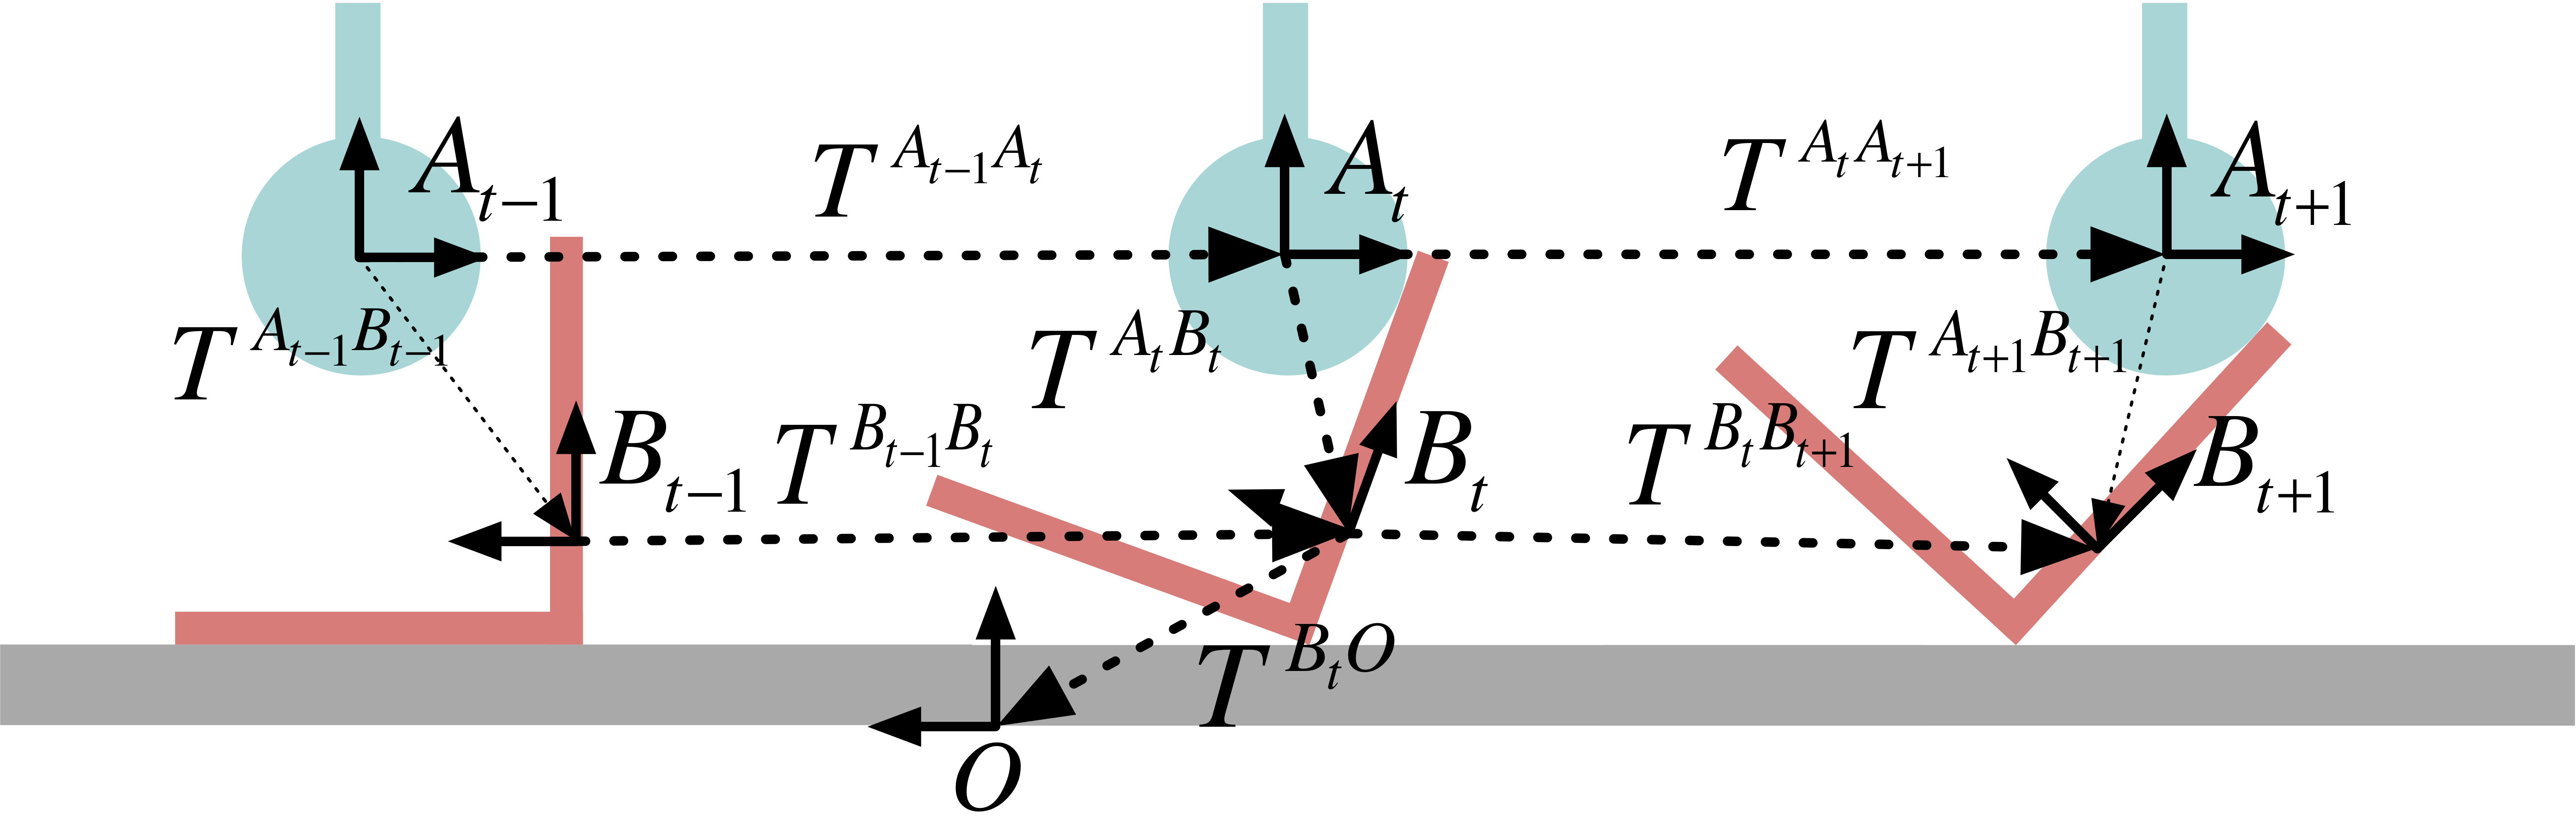
\includegraphics[width=0.67\textwidth]{sequential-frames}
%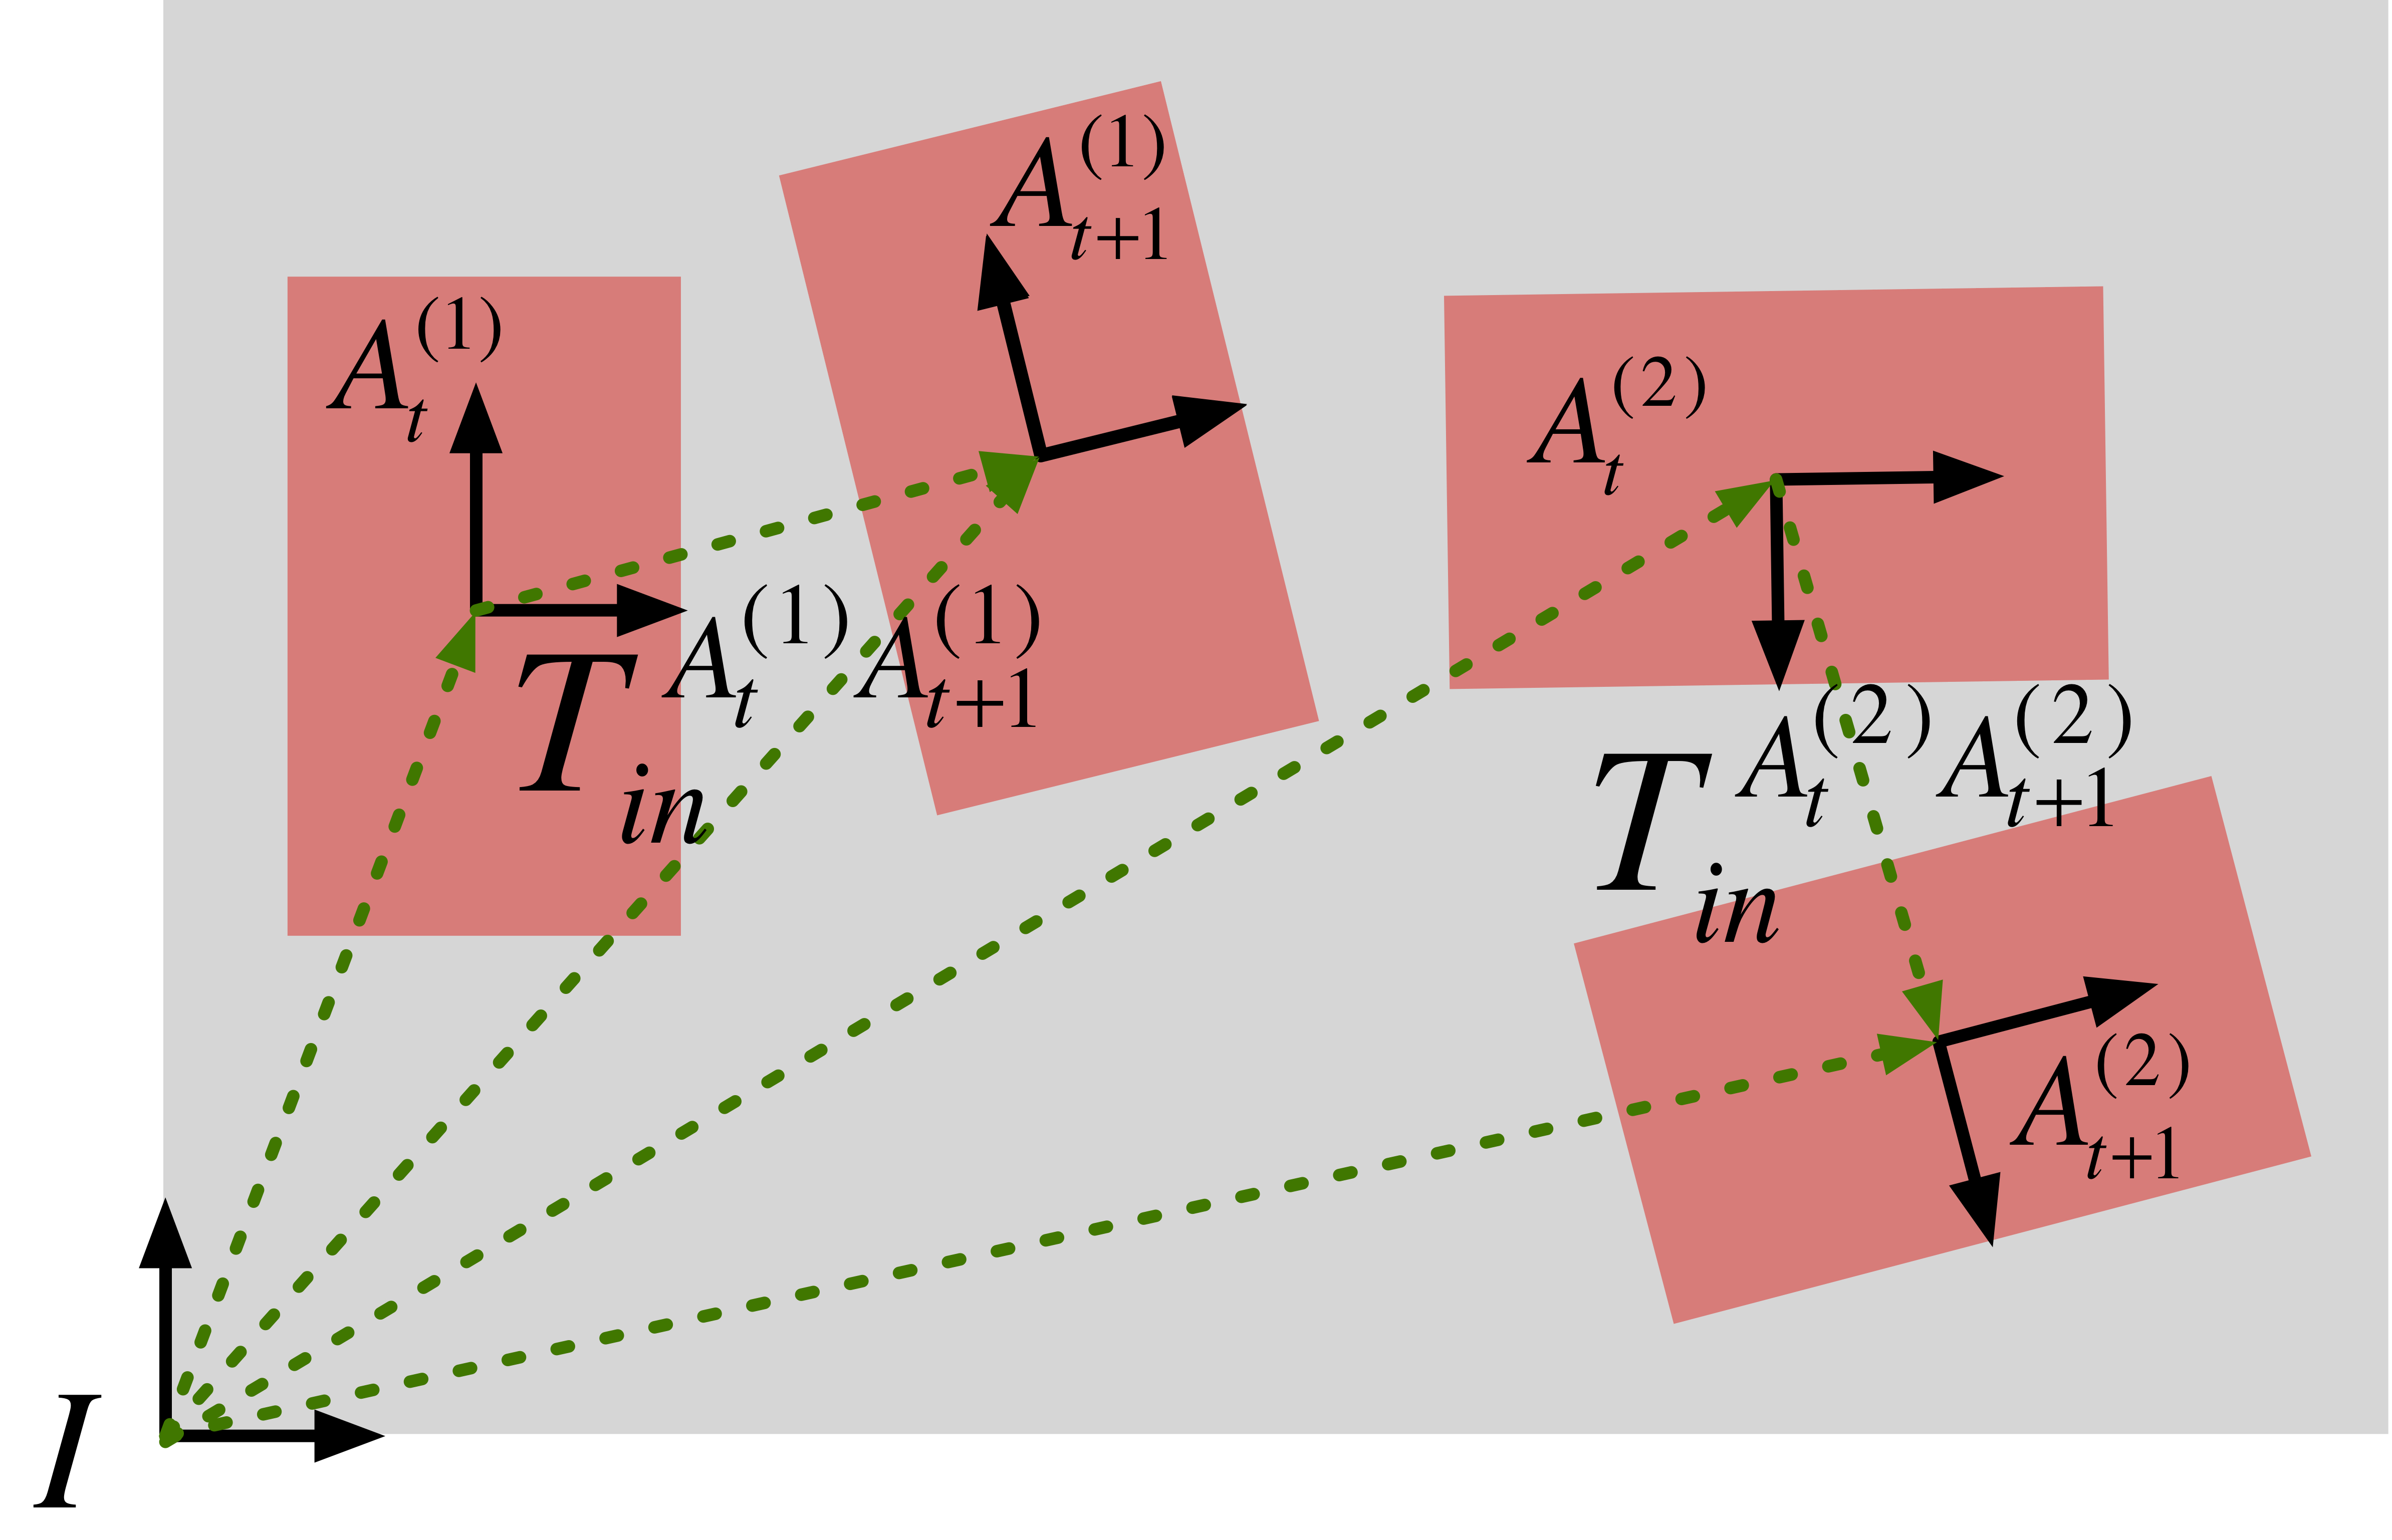
\includegraphics[width=0.34\textwidth]{similarity}
}
\caption[Setup1]{2D projection at time $t$ of a robotic finger with frame at time $t$ of $A_{t}$,
an object with frame $B_{t}$, and a ground plane with constant frame
$O$. Over three time steps this system consists can be described by six rigid body transformations %$T^{A_t, B_t}$, $T^{B_t, O}$, $T^{A_{t-1}, A_{t}}$, $T^{A_{t}, A_{t+1}}$, $T^{B_{t-1}, B_{t}}$, and $T^{B_{t}, B_{t+1}}$.
}
\label{fig:Learning.setup1}
\end{figure*}

\section{Encoding rigid body kinematics}
\label{sec:Representations}

In this section we set up the basic notation required to pose the
above prediction learning problems formally. Without loss of generality we explain the notation using an example from our application domain
(Figure~\ref{fig:Learning.setup1}). Three reference frames $A$, $B$
and $O$ sit in a $3$\nobreakdash-\hspace{0pt}dimensional Cartesian
space. Frame $A$ is attached to a robot finger which pushes an object with frame $B$, which in turn is placed on a table top with frame
$O$.\footnote{Although it is an abuse of notation for brevity we will
  use $A$, $B$ and $O$ to denote either the frame or the body to which  it is attached. So we will talk both of the frame $B$ and the object $B$.} While frame $O$ is fixed, $A$ and $B$ change in time and are observed at discrete time steps $..., t-1, t, t+1, ...$.  Frame $X$ at
time step $t$ is denoted $X_t$, and the rigid body transformation
between a frame $X$ and a frame $Y$ is denoted by $T^{X, Y}$.

From classical mechanics we know that in order to predict the change
in state of a rigid body, it is sufficient to know its mass, velocity
and a net force applied to the body.  Since our method will rely on
learning from object trajectories we cannot assume any knowledge of
the mass and applied forces. We can however, use the motion of a body over time to encode acceleration -- an effect of the applied net
force. We therefore use rigid body transformations $T^{X,Y}$ of the interacting bodies through time (Figure~\ref{fig:Learning.setup1}). Given the additional assumption that the net force and the body mass are constant, two subsequent rigid body transformations $T^{B_{t-1},
  B_{t}}$ and $T^{B_{t},B_{t+1}}$ give a complete description of the
state of some body B (here the object) at time step $t$ in the absence
of the other bodies.  Adding the transformation $T^{B_t, O}$ to give a
triple of transformations thus provides a complete description of the
state of body B in the fixed frame $O$ (the stationary elements of the
environment).  Similarly, a second triple of transformations $T^{A_t,
  O}$, $T^{A_{t-1}, A_{t}}$ and $T^{A_{t}, A_{t+1}}$ provides such a
description for some other body (here the finger) with frame $A$. 
The state of the overall system consisting of these two interacting
bodies with frames $A$ and $B$ and the fixed environment $O$ can
thus be adequately described by these six transformations.

In fact in our representation, we replace transformation $T^{A_t, O}$ by relative transformation $T^{A_t, B_t}$, thus also explicitly capturing the spatial relationship and thus any contacts between $A$ (finger) and $B$ (object). This gives us a representation consisting of the set of six transformations marked in bold dotted lines in Figure~\ref{fig:Learning.setup1}. The prediction problem, simply put, will thus be to predict the motion of the object $B$ in the next step: $T^{B_t,B_{t+1}}$ given these five other transformations. Before defining the problem formally, however, we need to think briefly about how best to store these transformations.

Specifically, since we are interested in learning, we need to express this set of transformations in a way that supports generalised predictions. In general the behaviours of interacting bodies described by frames from Figure~\ref{fig:Learning.setup1} are independent of any inertial frame \cite{kopicki_prediction_2010}. Unfortunately, a na\"{\i}ve representation of transformation $T^{A_{t}, A_{t+1}}$ as $A_{t+1}(A_{t})^{-1}$, or explicitly given inertial frame $I$,
% MAREK CHECK
\begin{equation}
T_{in}^{A_{t}, A_{t+1}} = T^{I, A_{t+1}} (T^{I, A_{t}})^{-1}
\label{eq:Learning.In1}
\end{equation}
\noindent makes the transformation in \eqref{eq:Learning.In1} dependent on the currently used inertial frame $I$ (see
Figure~\ref{fig:similarity}).  This would make the stored transformations poor from the point of view of generalisation. A better way is instead to store all the transformations in a body frame (at learning time) and convert to and from an inertial frame dependent transformation (at prediction time) using similarity transforms.

\begin{figure}[b!]
\centerline{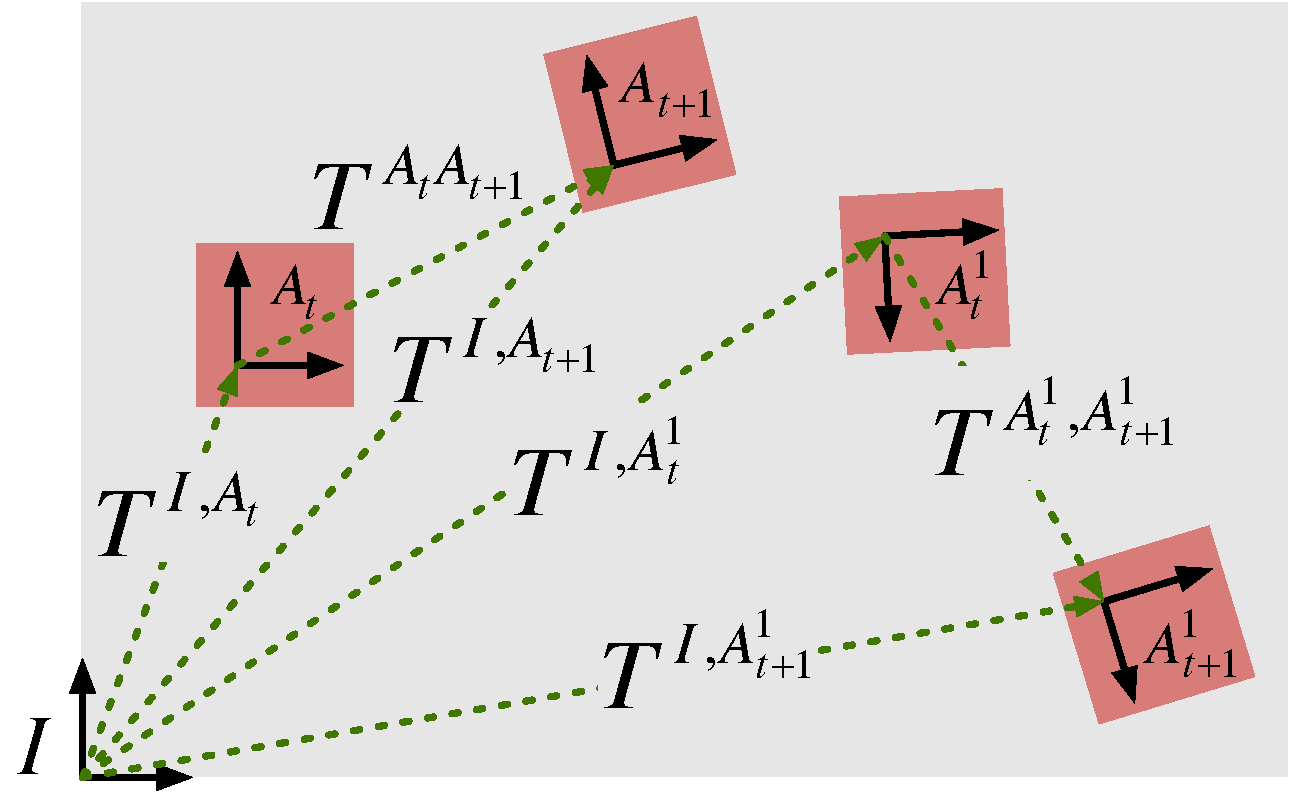
\includegraphics[width=0.85\columnwidth]{similarity-new}}
\caption[Similarity]{ Overhead view of an object on a table starting in two different positions. In each case the motion from $t$ to $t+1$ is the same relative to the instantaneous object body frames $A$ and $A^{1}$. However because transformations $T^{I, A}$ and $T^{I, A^{1}}$ are different, the corresponding transformations in the inertial frame are also different, i.e.\ $T_{in}^{A_{t}, A_{t+1}} \neq T_{in}^{A^{1}_{t}, A^{1}_{t+1}}$.}
\label{fig:similarity}
\end{figure}
Intuitively these similarity transforms align the inertial and body frames, perform the required transformation and then invert the transformation required to align them. In this manner, given the instantaneous object frame $A_{t}$ at time $t$, and the inertial frame dependent transformation
$T_{in}^{A_{t}, A_{t+1}}$, one can obtain the body frame dependent
transformation $T_{body}^{A_{t}, A_{t+1}}$:

\begin{equation}
T_{body}^{A_{t}, A_{t+1}} = (T^{I, A_{t}})^{-1} T_{in}^{A_{t}, A_{t+1}} T^{I, A_{t}}
\label{eq:Learning.Body1}
\end{equation}

\noindent where $T^{I, A_{t+1}} =$ $T_{in}^{A_{t}, A_{t+1}} T^{I, A_{t}} =$ $T^{I, A_{t}} T_{body}^{A_{t}, A_{t+1}}$.

It is this body frame dependent transformation that will be stored during learning. Conversely, when a prediction is required, given a body frame dependent transformation, the object
frame $A_{t}$, and using Equation~\eqref{eq:Learning.Body1}, the
inertial frame dependent transformation $T_{in}^{A_{t}, A_{t+1}}$ is
recovered using:
\begin{equation}
T_{in}^{A_{t}, A_{t+1}} = T^{I, A_{t}} T_{body}^{A_{t}, A_{t+1}} (T^{I, A_{t}})^{-1}
\label{eq:Learning.Body2}
\end{equation}
This technique is critical to generalisation across inertial frames. In the rest of the paper we will retain subscripts $in$, but suppress subscripts $body$, and assume that all transformations $T^{X, Y}$ are transformations in the body frame $X$ related to the equivalent transform in some inertial frame using a similarity transform:
\begin{equation}
T^{X, Y} \equiv T_{body}^{X, Y} = ({T^{I, X}})^{-1} T_{in}^{X, Y} {T^{I, X}}
\label{eq:Learning.Similarity}
\end{equation}

\section{Formal statement: learning to predict}
\label{sec:PredictionProblem}

We now have the basics required to formally describe the one-step and then the multi-step prediction
problem in such a way that they become problems of learning to predict, and we can effectively tackle Problem 1 (Action Interpolation).

\noindent {\bf One step prediction.} The one step prediction problem is formulated as follows: given that we observe the recent and current positions of the finger and object, and know the planned motion of the finger, $T^{A_{t},  A_{t+1}}$, predict the resulting immediate motion of the object,
$T^{B_{t}, B_{t+1}}$.  This is a problem of finding a function~$f$:
\begin{multline}
f: T^{A_t, B_t}, T^{B_t, O}, T^{A_{t-1}, A_{t}}, T^{B_{t-1}, B_{t}}, T^{A_{t}, A_{t+1}} \\ \longrightarrow T^{B_{t}, B_{t+1}}
\label{eq:Learning.long}
\end{multline}

The function $f$ is capable of describing the effects of interactions between rigid bodies $A$ and $B$, providing their physical properties and net forces are constant
in time,\footnote{A dynamic formulation could explicitly incorporate
net forces into the domain and codomain of \eqref{eq:Learning.long}.}
in the limit of infinitesimally small time steps.
Furthermore, it can be approximately learned from observations
for some small fixed time interval $\Delta t$ between time steps.

If robotic manipulations are performed slowly we can assume quasi-static conditions, and ignore all frames at time $t-1$.  This conveniently reduces the dimensionality of the problem, giving a simplified function~$f_{qs}$:
\begin{equation}
f_{qs}: T^{A_t, B_t}, T^{B_t, O}, T^{A_{t}, A_{t+1}} \longrightarrow T^{B_{t}, B_{t+1}}
\label{eq:Learning.short}
\end{equation}

\noindent {\bf Multi-step prediction.} Having stated the one-step prediction problem it is possible to solve
the multi-step prediction problem. Given a predictor (either $f$ or
$f_{qs}$), the initial state of the finger $T^{A_{1}, O}$ and object
$T^{B_{1}, O}$, and knowing the trajectory of the finger $A_{1},
\ldots A_{T}$ over $T$ time steps, one can predict the complete
trajectory of the object $B_{1}, \ldots B_{T}$, by simply iterating
the predictions obtained from $f_{qs}$.  That is, the output of the
predictor at time~$t$ is used as the input to the predictor for the
next time step (Figure~\ref{fig:three-prediction-problems}).

\noindent {\bf Learning to predict as regression.} In principle it is straightforward to acquire a predictor $f$ or
$f_{qs}$ by learning it from data. Given sufficient experience of
object and finger trajectories we can perform a nonparametric
regression analysis by taking $T^{A_t, B_t}, T^{B_t, O}, T^{A_{t},
  A_{t+1}}$ as independent variables, and $T^{B_{t}, B_{t+1}}$
as the dependent variable.  Nonetheless a powerful regression
technique is needed since the domain of $f_{qs}$ has 18~dimensions
or more depending on the parameterisation of motion.

\noindent {\bf Learning to predict as density estimation.} As an alternative to learning the mapping~\eqref{eq:Learning.short} by regression, we can recast $f_{qs}$ as a conditional probability density (CPD) $p_{qs}$ over possible object motions $T^{B_{t},B_{t+1}}$~\cite{kopicki_prediction_2009}:
\begin{equation}
p_{qs}(T^{B_{t}, B_{t+1}} | T^{A_t, B_t}, T^{B_t, O}, T^{A_{t}, A_{t+1}})
\label{eq:Learning.density1}
\end{equation}

The learning problem is then posed as one of density estimation, permitting the modelling of the probabilities of many possible outcomes. 

Either the regression or density estimation formulation can be used in a modular scheme. In that case a separate module is learned for each agent-object-environment combination. Each module interpolates over actions for its context, and thus the system solves problem P1: Action Interpolation for multiple contexts. There is not, however, enough information in the five transformations used as input, to solve either problem P2 (Action Transfer) or problem P3 (Shape Transfer). We now identify the additional information needed to solve these.

\section{Transfer Learning: Representing contacts}
\label{sec:InfoForPrediction}

The input domains of $f$, $f_{qs}$ $p_{qs}$ as proposed above  adequately represent the behaviour of a specific pair of rigid bodies in a specific environment. They thus provide a well posed version of problem P1 (Action Interpolation). Given this information, however, we cannot solve problems P2 (Action Transfer) or P3 (Shape Transfer). This is because there is insufficient information: the input variables only capture {\em global} relations between objects. To properly pose transfer learning problems we must also explictly capture in the input domain all the {\em local} contact relations between the object and its surroundings. 

\begin{figure}[t]
\centerline{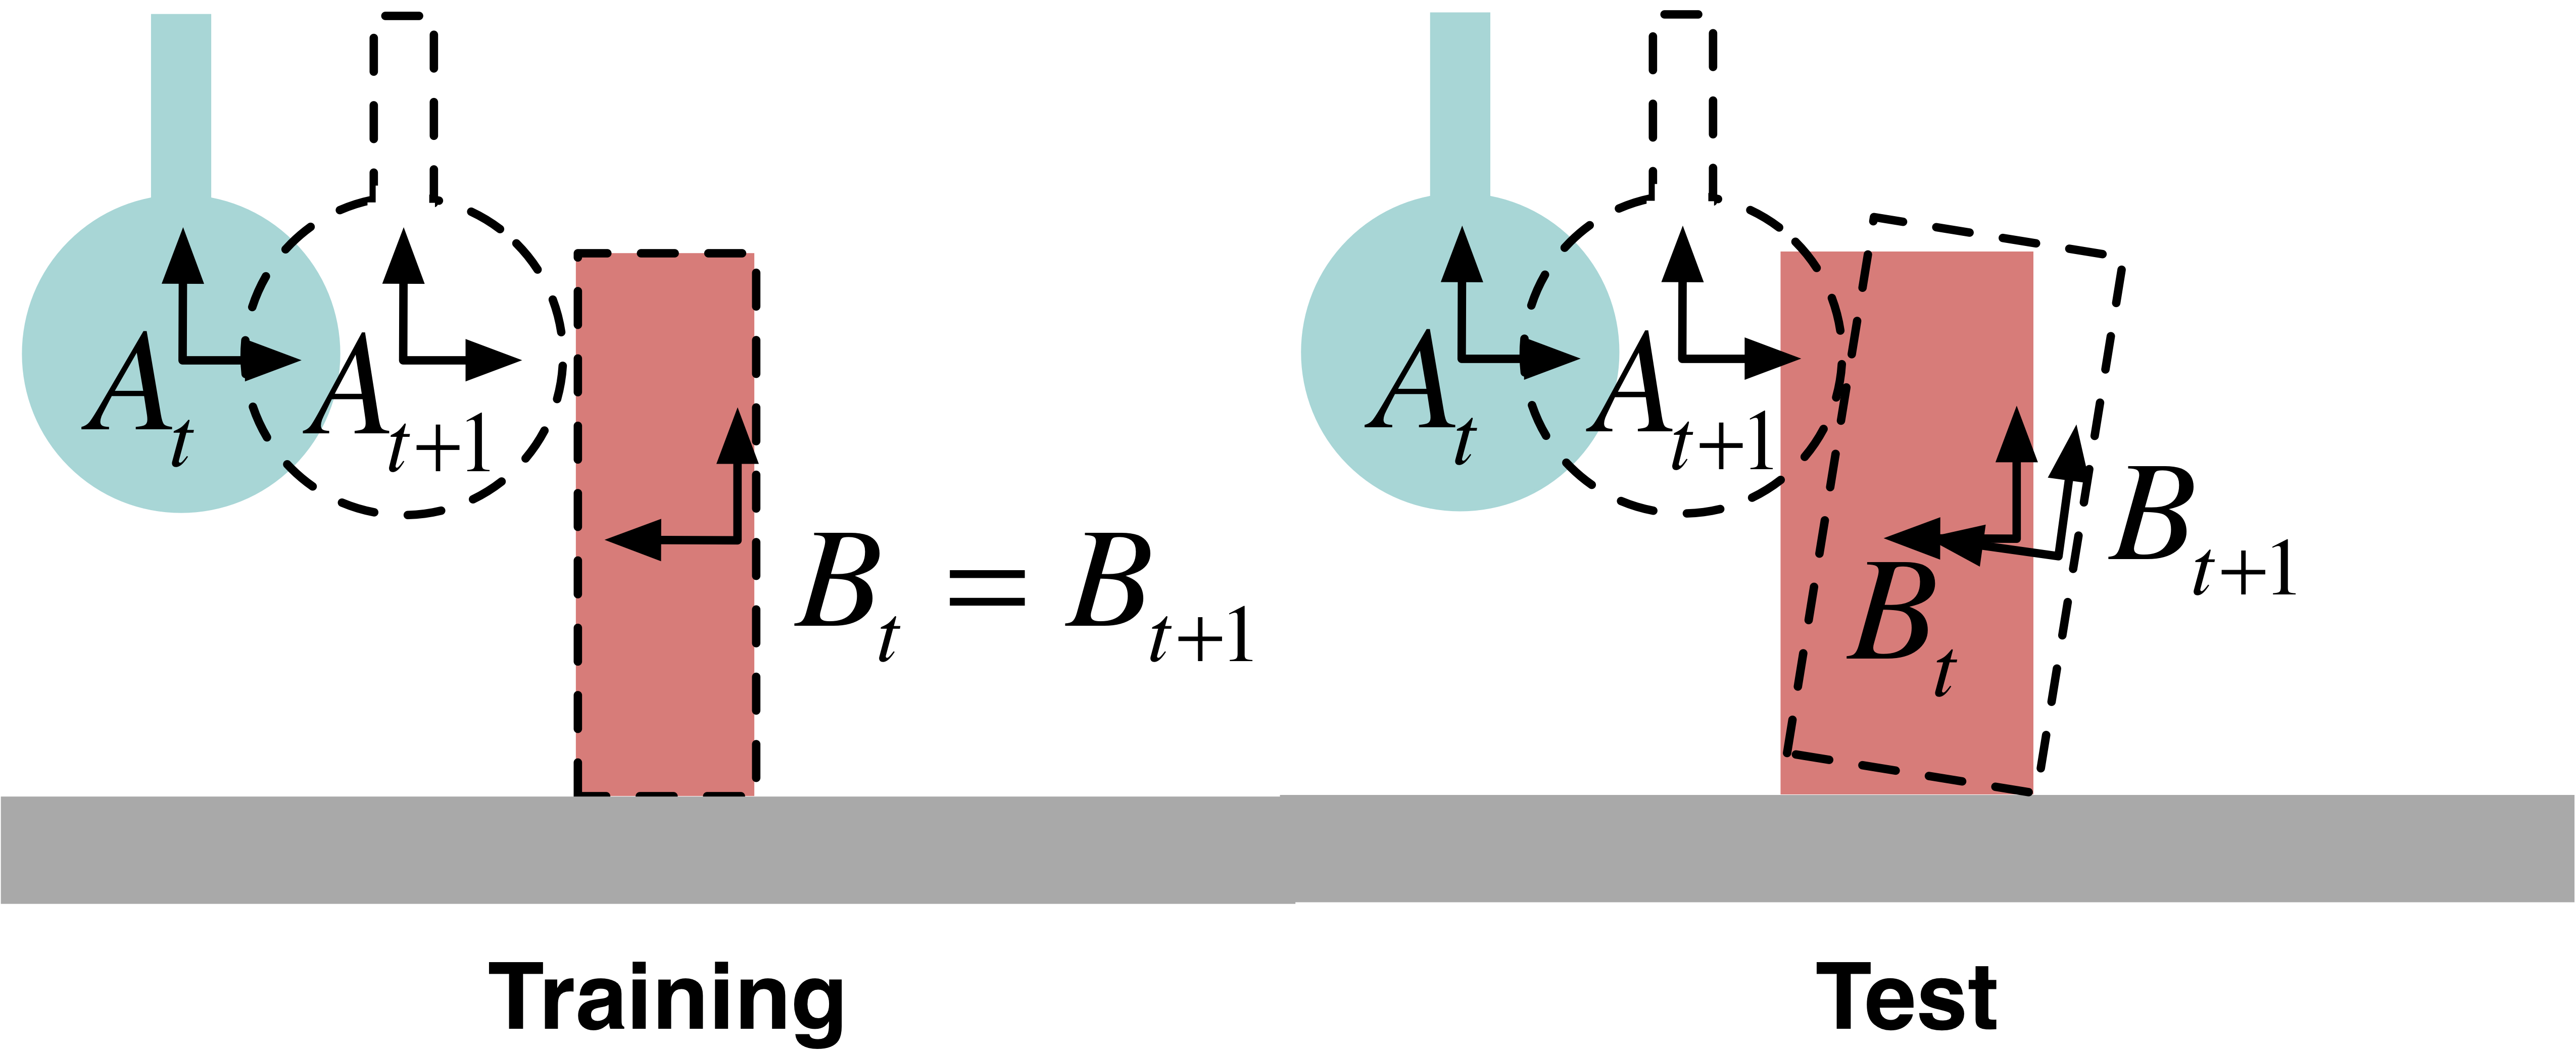
\includegraphics[width=7.5cm]{shapes-colour}}
\caption[Shapes]{Two scenes (left and right),
each with an object on a tabletop, and a finger.
Only the shape of object B differs between the scenes.
Yet when A moves to the position shown by the dashed outline at time $t+1$,
the resulting displacement of B
(represented by the transformation $T^{B_{t}, B_{t+1}}$)
will be quite different.}
\label{fig:Learning.shapes}
\end{figure}

To see why, consider a simple case of shape transfer in Figure~\ref{fig:Learning.shapes}. On the left is a training example. On the right is a test case, where the only difference is that the shape of the object has changed: it is wider. Given the same placement of the frames on object and agent, and the same finger motion, the predicted behaviour using Equation~\eqref{eq:Learning.short} must be the same as for the training example. But this is wrong. To enable the correct prediction to be transferred, additional information is needed in the input domain. Specifically, information on the contact between $A$ and $B$ is required. This can be captured by attaching additional frames to $A$ and $B$ close to their point of contact (see Figure~\ref{fig:Learning.setup2} (centre panel)).

In general an object will have multiple contacts with both the robot, and the environment. Each of these contacts provides a kinematic constraint on the motion of the object, and thus each one of these contacts should be captured as input variables. Only in this way does the predictor have sufficient information to solve transfer problems P2 and P3. Rigid body simulators employ just such contact information. 

%.  A predictor based on
%Equation~\eqref{eq:Learning.short}, and trained on the smaller object
%$B$ (Figure~\ref{fig:Learning.shapes} left scene), cannot generalise
%to the larger object (right scene). This is because the three input
%reference frames ($A_t$, $B_t$, $A_{t+1}$) in the left and right
%panels have identical poses. Thus the predictions will be identical
%even though the shapes are different. For the right panel the
%prediction will be that the finger $A$ will pass into object $B$. So,
%as posed there is insufficient information in the domain of the
%function to allow generalisation. To enable such generalisation
%information on the contact between $A$ and $B$ is required. If object
%$B$ has multiple contacts then information on all of them should be
%included. Physics simulators employ just such contact information to
%inform their predictions. 

\begin{figure*}[t]
\centerline{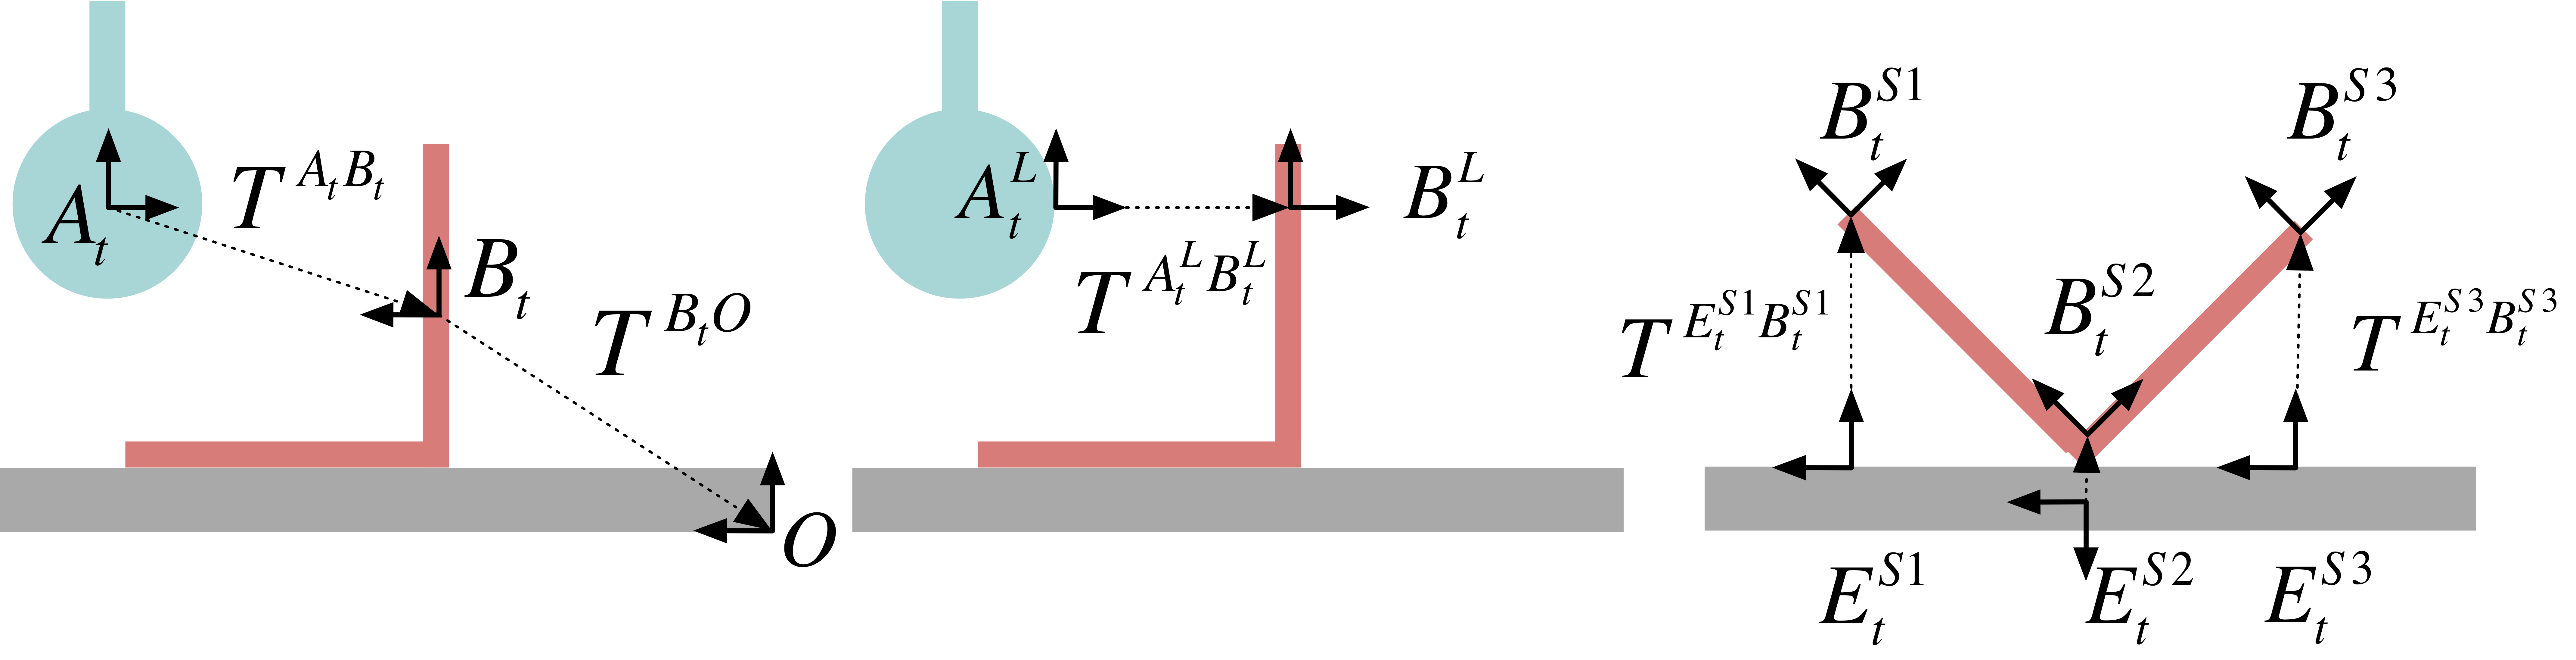
\includegraphics[width=0.75\textwidth]{information}}
\caption{Three types of information useful in prediction problems. Left: (G - global) global frames of reference for the robot, object and the world. Centre: (A - agent) local frames of reference on the robot finger and the closest point on the object. Right (E - environment) local frames of reference on the object and the closest points on surfaces in the environment.}
\label{fig:Learning.setup2}
\end{figure*}

Our approach is to use a pair of local frames to encode each contact or near contact. Each pair encodes one transformation between part of the object $B$ and another body.  To distinguish these local frame pairs from what has gone before we henceforth refer to the main frame attached to each body (as defined in Section~\ref{sec:Representations}) as the global frame for that body. 

We can formally define these local frame pairs as follows. Reconsider
the 2D projection of a robot finger with global frame $A_{t}$, an
object with global frame $B_{t}$, and the environment global frame $O$
(Figure~\ref{fig:Learning.setup2}, left panel). We now also define a pair of local frames
capturing the finger-object contact as $A^{L}_{t}$ and
$B^{L}_{t}$ (centre panel). These are spatially dynamic, i.e.\ at any time $t$ they
are located at the points of closest proximity on the finger and
object respectively.  We define the \textit{agent-object contact}
information as the transformations $T^{A^{L}_{t}, A^{L}_{t+1}}$ and
$T^{A^{L}_t, B^{L}_t}$.

We additionally define $N$ pairs of local frames $B^{Sk}_t$ and $E^{Sk}_t$ to
capture the object-environment contacts, where ($k=1 \ldots N$) (Figure~\ref{fig:Learning.setup2} right panel). We attach the $N$ frames $B^{Sk}_t$
to various parts of the object. Each has a corresponding frame in the
environment $E^{Sk}_t$.  Because they are spatially dynamic the
frames $E^{Sk}_t$ move over surfaces in the environment, as the
object moves. We define the \textit{object-environment contact}
information as the set of transformations $T^{E^{Sk}_t,B^{Sk}_t}$ for $k=1
\ldots N$. To obtain the results presented in this paper, the number and the
locations of the frames $B^{Sk}_t$ on each different object were
determined by hand. In principle this procedure could be automated,
but falls beyond the scope of the current work.

We have already motivated the need for these additional input
variables to support shape generalisation. Their utility can also be seen with respect to changes in
action. The top row of Figure~\ref{fig:ToyExample} shows a training
and a test case for problem P2 (action transfer). The prediction of the test push trajectory requires some encoding of the kinematic constraint
imposed by the contact between the base of the L-shaped flap and the
table. This constraint exists in the training push, but is not
significant since the flap can rotate around its corner, unconstrained
by the base.

\begin{figure}[b]
\centerline{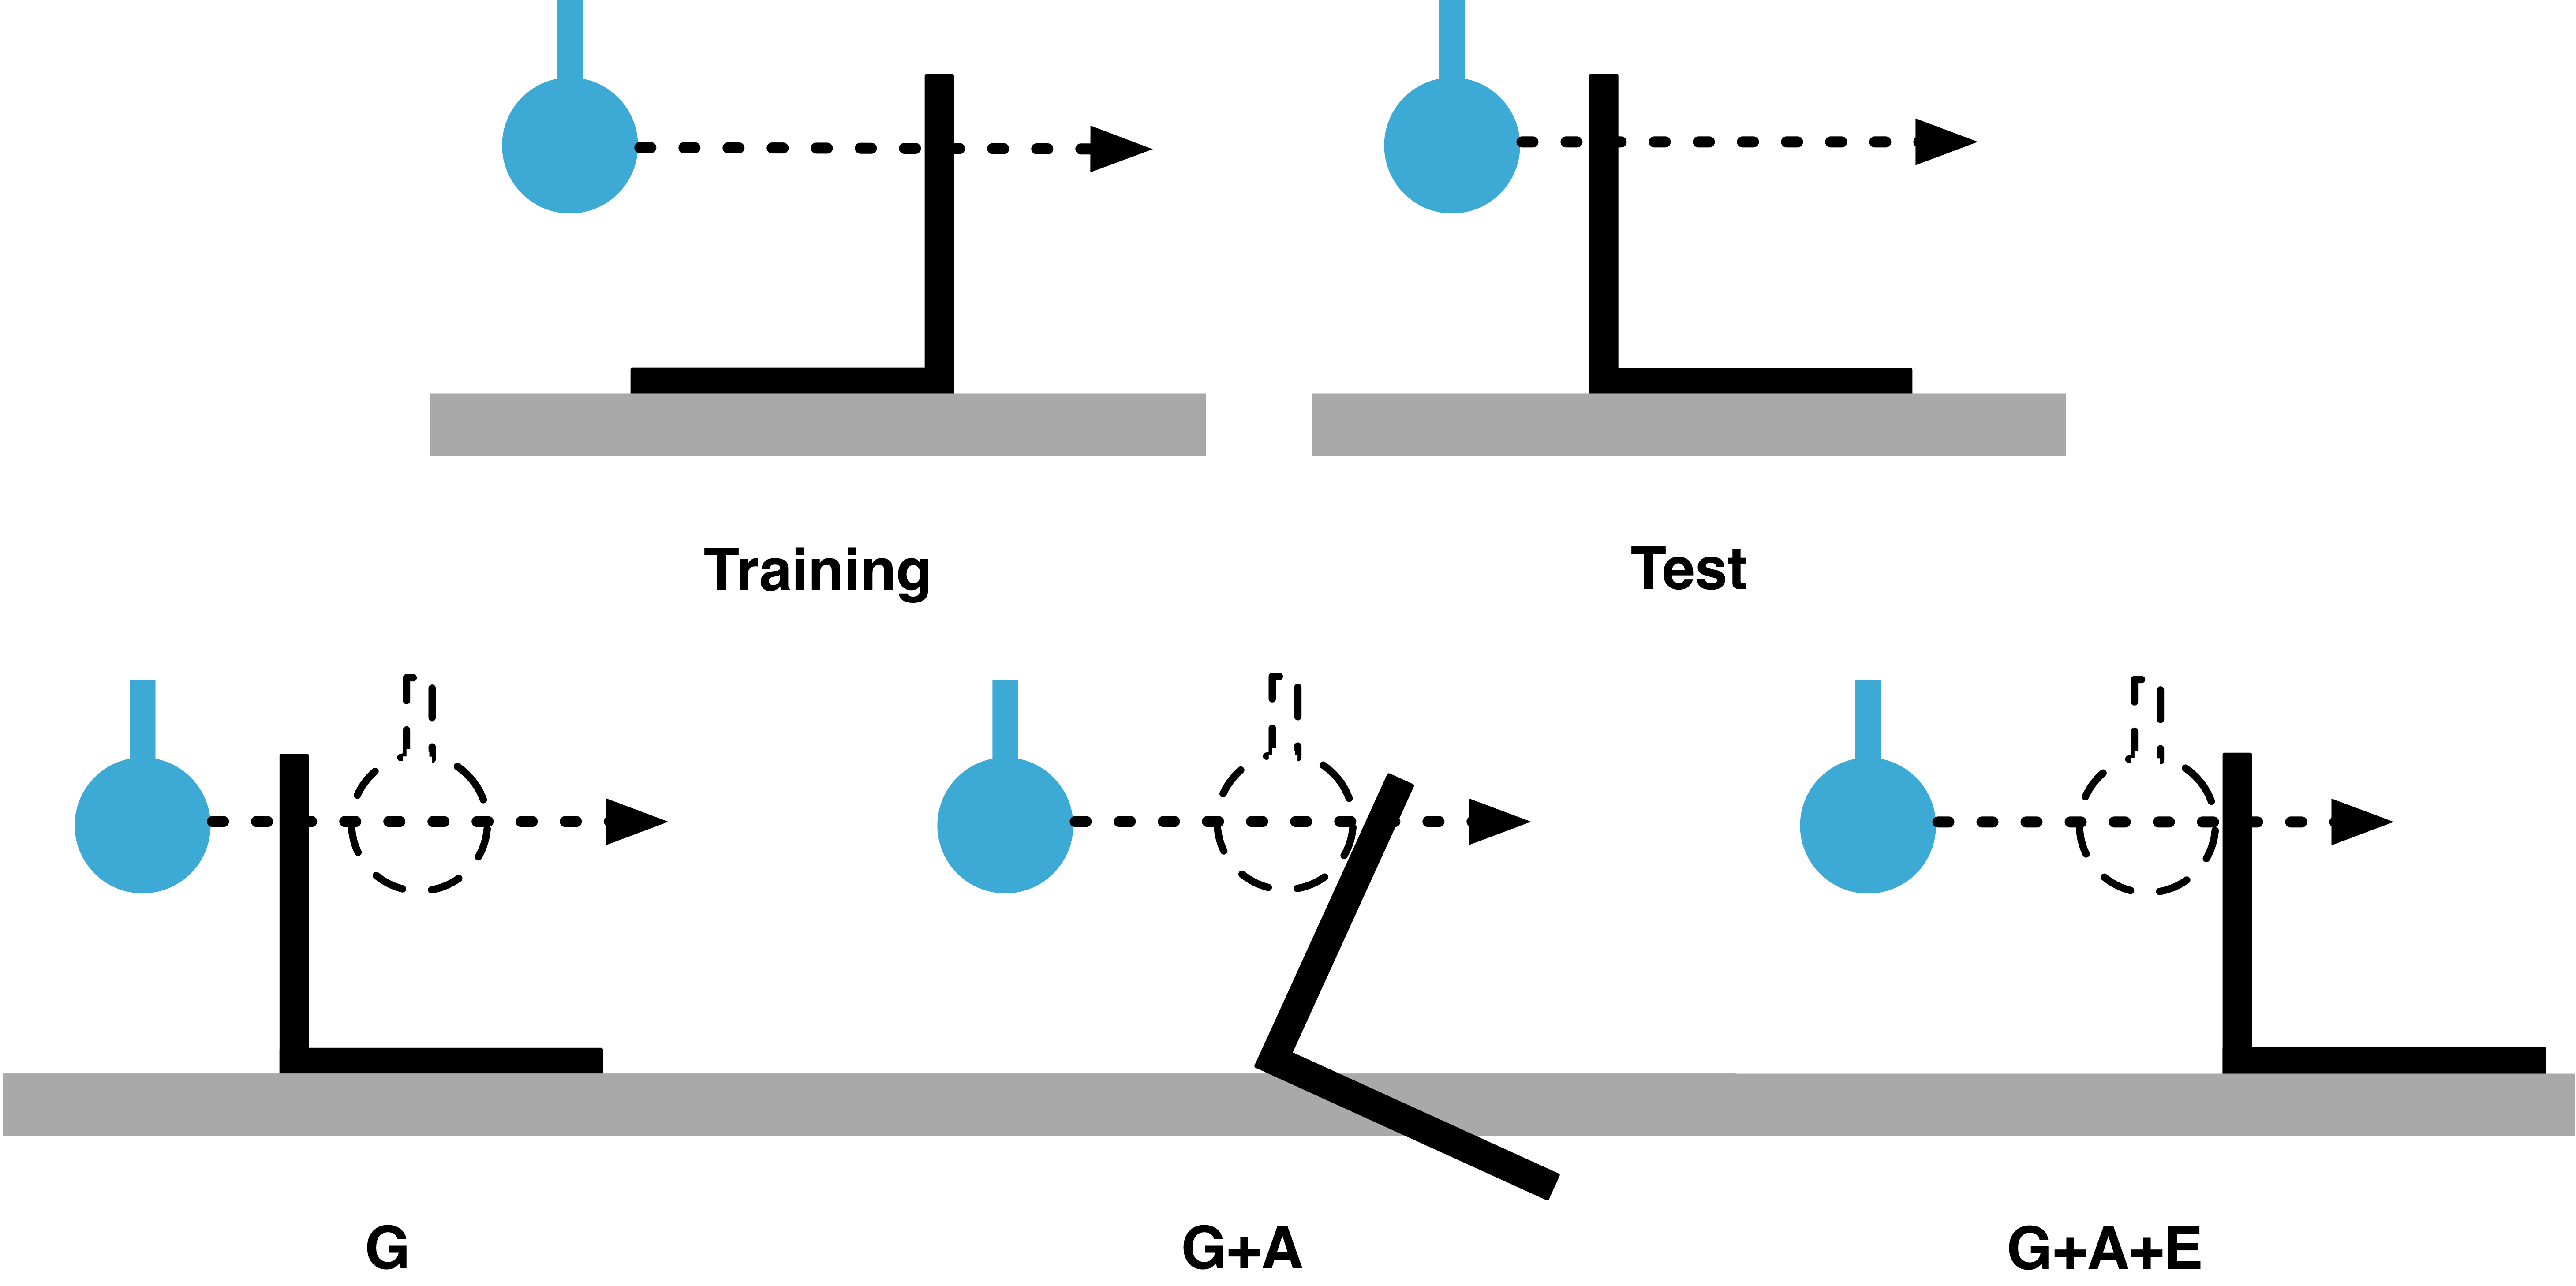
\includegraphics[width=0.8\columnwidth]{BackPushToyExample}}
\caption[ToyExample]{Schematic diagram (2D projection of 3D scene)
in which an object (of L-shaped cross-section) on a supporting surface
is pushed by a robotic finger. 
Various predictors are trained solely on forward pushes (top left), but tested on backwards pushes (top right). The top panels show the push trajectory for the training and test phases, whereas the bottom panels show the outputs from three types of predictor (G, G+A and G+A+E) in the test phase.}
\label{fig:ToyExample}
\end{figure}

We can now consider the effects that different amounts of information
might have on generalised predictions. A predictor endowed only with
information based on the global frames for each body we refer to as
having global information (G). We can add agent-object contact
information to this (G+A), and in turn we can add object-environment
contact information (G+A+E). Now consider the possible predictions for
the test case (Figure~\ref{fig:ToyExample} bottom row). A predictor
using G will predict that the object will not move, because it has no
nearby experience to suggest otherwise. A predictor using G+A has
information from the training case that the object surface will move
with the finger, so that the finger will not pass through it, but is
also capable of predicting that the object rotates about the corner
and into the table since it doesn't model the object-environment
contact. A predictor using G+A+E will have information about the
effect of the contact between the base of the flap and the table and
so should avoid predicting a rotation into the table.

One point is critical here: the above analysis only concerns what the
information allows, it depends on the ability of the learner to
utilise it.  To test this we must incorporate the information into
each learning framework. We can simply extend the regression and density
estimation frameworks to achieve this. For regression one way to
incorporate the extra information $A^{L}_{t}$,$B^{L}_{t}$ and
$E^{Sk}_t$\hspace{-6pt}, $B^{Sk}_t$, provided by the agent and
environment contacts, is simply to enlarge the domain of function~$f$
in Equation~\eqref{eq:Learning.short}, that is:
\begin{multline}
f'_{qs}: T^{A_t, B_t}, T^{B_t, O}, T^{A_{t}, A_{t+1}}, T^{A^{L}_t, B^{L}_t}\{, T^{E^{Sk}_t,B^{Sk}_t}\}_{k=1 \ldots N} \\ 
\longrightarrow T^{B_{t}, B_{t+1}}
\label{eq:Learning.augmented}
\end{multline}

\noindent Unfortunately, because the dimensionality of the domain of $f'_{qs}$ grows with the number of environment contacts $N$,
the difficulty of learning the mapping $f'_{qs}$ rapidly increases
as more environment contacts are added.


The conditional probability density (CPD) $p_{qs}$ over possible object motions $T^{B_{t}, B_{t+1}}$~\cite{kopicki_prediction_2009} is augmented as follows:
\begin{multline}
p_{qs}(T^{B_{t}, B_{t+1}} | T^{A_t, B_t}, T^{B_t, O}, T^{A_{t}, A_{t+1}}, T^{A^{L}_t, B^{L}_t}\\
\{, T^{E^{Sk}_t,B^{Sk}_t}\}_{k=1 \ldots N})
\label{eq:Learning.density}
\end{multline}

Again the dimensionality of the conditioning variables makes density
estimation hard as the number of contacts grows. One way round this in the density estimation case is to factorize the density in a way that
reflects the contact structure. We consider this in the next section. 

\section{Factorised density estimation}
\label{sec:Factors}

Both formulations give learning problems that increase in difficulty as further contacts are added. One question is whether either formulation can be recast so as to take advantage of the natural
problem structure. This section presents one such scheme for the
density estimation (or CPD) formulation, based on a product of experts.

Specifically the CPD formulation allows us to factorise the density
and approximate $p_{qs}$ by making a conditional independence
assumption. The unfactored CPD formulation gives a density over
possible one step motions of the object. We can
factorise this by breaking up the conditioning variables into groups
according to the contacts. This reflects the notion that the behaviour
at one contact is independent of the other contacts: each component of the
product is an expert encoding the likely object motions given a single
kinematic constraint. The product will be maximised by a
motion that best satisfies all the constraints simultaneously.

The computational advantage is that since the component
densities factorise the conditioning variables of $p_{qs}$ their
domains' dimensionalities are smaller, and so potentially they can
better manage the complexity of incorporating more information into
the predictor.  Furthermore, the subset of experts used in the product can be selected dynamically, depending for example on the current set of contacts. Schematically, for some normalisation constant~$C$ we propose the following factorisation:
\begin{equation}
p_{qs} \approx C\ p_{global}\ p_{agent}\ \mathop{\prod}_{k=1 \ldots N}{ p_{env,k}}
\label{eq:Learning.product}
\end{equation}
\noindent where
\begin{subequations}
\begin{align}
p_{global} &\equiv p_{global}(T^{B_{t}, B_{t+1}}|T^{A_{t}, A_{t+1}}, T^{A_t, B_t}, T^{B_t, O})
\label{eq:Learning.densityglobal} \\
p_{agent} &\equiv p_{agent}(T^{B^{L}_{t}, B^{L}_{t+1}}|T^{A^{L}_{t}, A^{L}_{t+1}}, T^{A^{L}_t, B^{L}_t})
\label{eq:Learning.densitylocal} \\
p_{env,k} &\equiv p_{env,k}(T^{B^{Sk}_t, B^{Sk}_{t+1}} | T^{E^{Sk}_t,B^{Sk}_t})
\label{eq:Learning.densityenv}
\end{align}
\end{subequations}

\noindent denote the \textit{global}, \textit{agent-object} and
$k^{th}$ \textit{object-environment} density factors
respectively~\cite{kopicki_prediction_2009}\cite{kopicki_prediction_2010}. 
The one step prediction problem can then be defined as finding the
transformation $\widetilde{T}_{in}^{B_{t}, B_{t+1}}$ expressed in some inertial frame which maximises the product of densities \eqref{eq:Learning.product}:
\begin{equation}
\widetilde{T}_{in}^{B_{t}, B_{t+1}} = \argmax{T_{in}^{B_{t}, B_{t+1}}} \bigg\lbrace
p_{global}\  p_{agent} \mathop{\prod}_{k=1 \ldots N}{ p_{env,k} }
\bigg\rbrace
\label{eq:Learning.MultiFactorProduct}
\end{equation}

\noindent where similarity transforms as described in Section~\ref{sec:Representations} must be used to evaluate $p_{global}$, $p_{agent}$ and the $N$ environment factors $p_{env,k}$ for a given ${T}_{in}^{B_{t}, B_{t+1}}$.
\begin{figure}[t]
\centerline{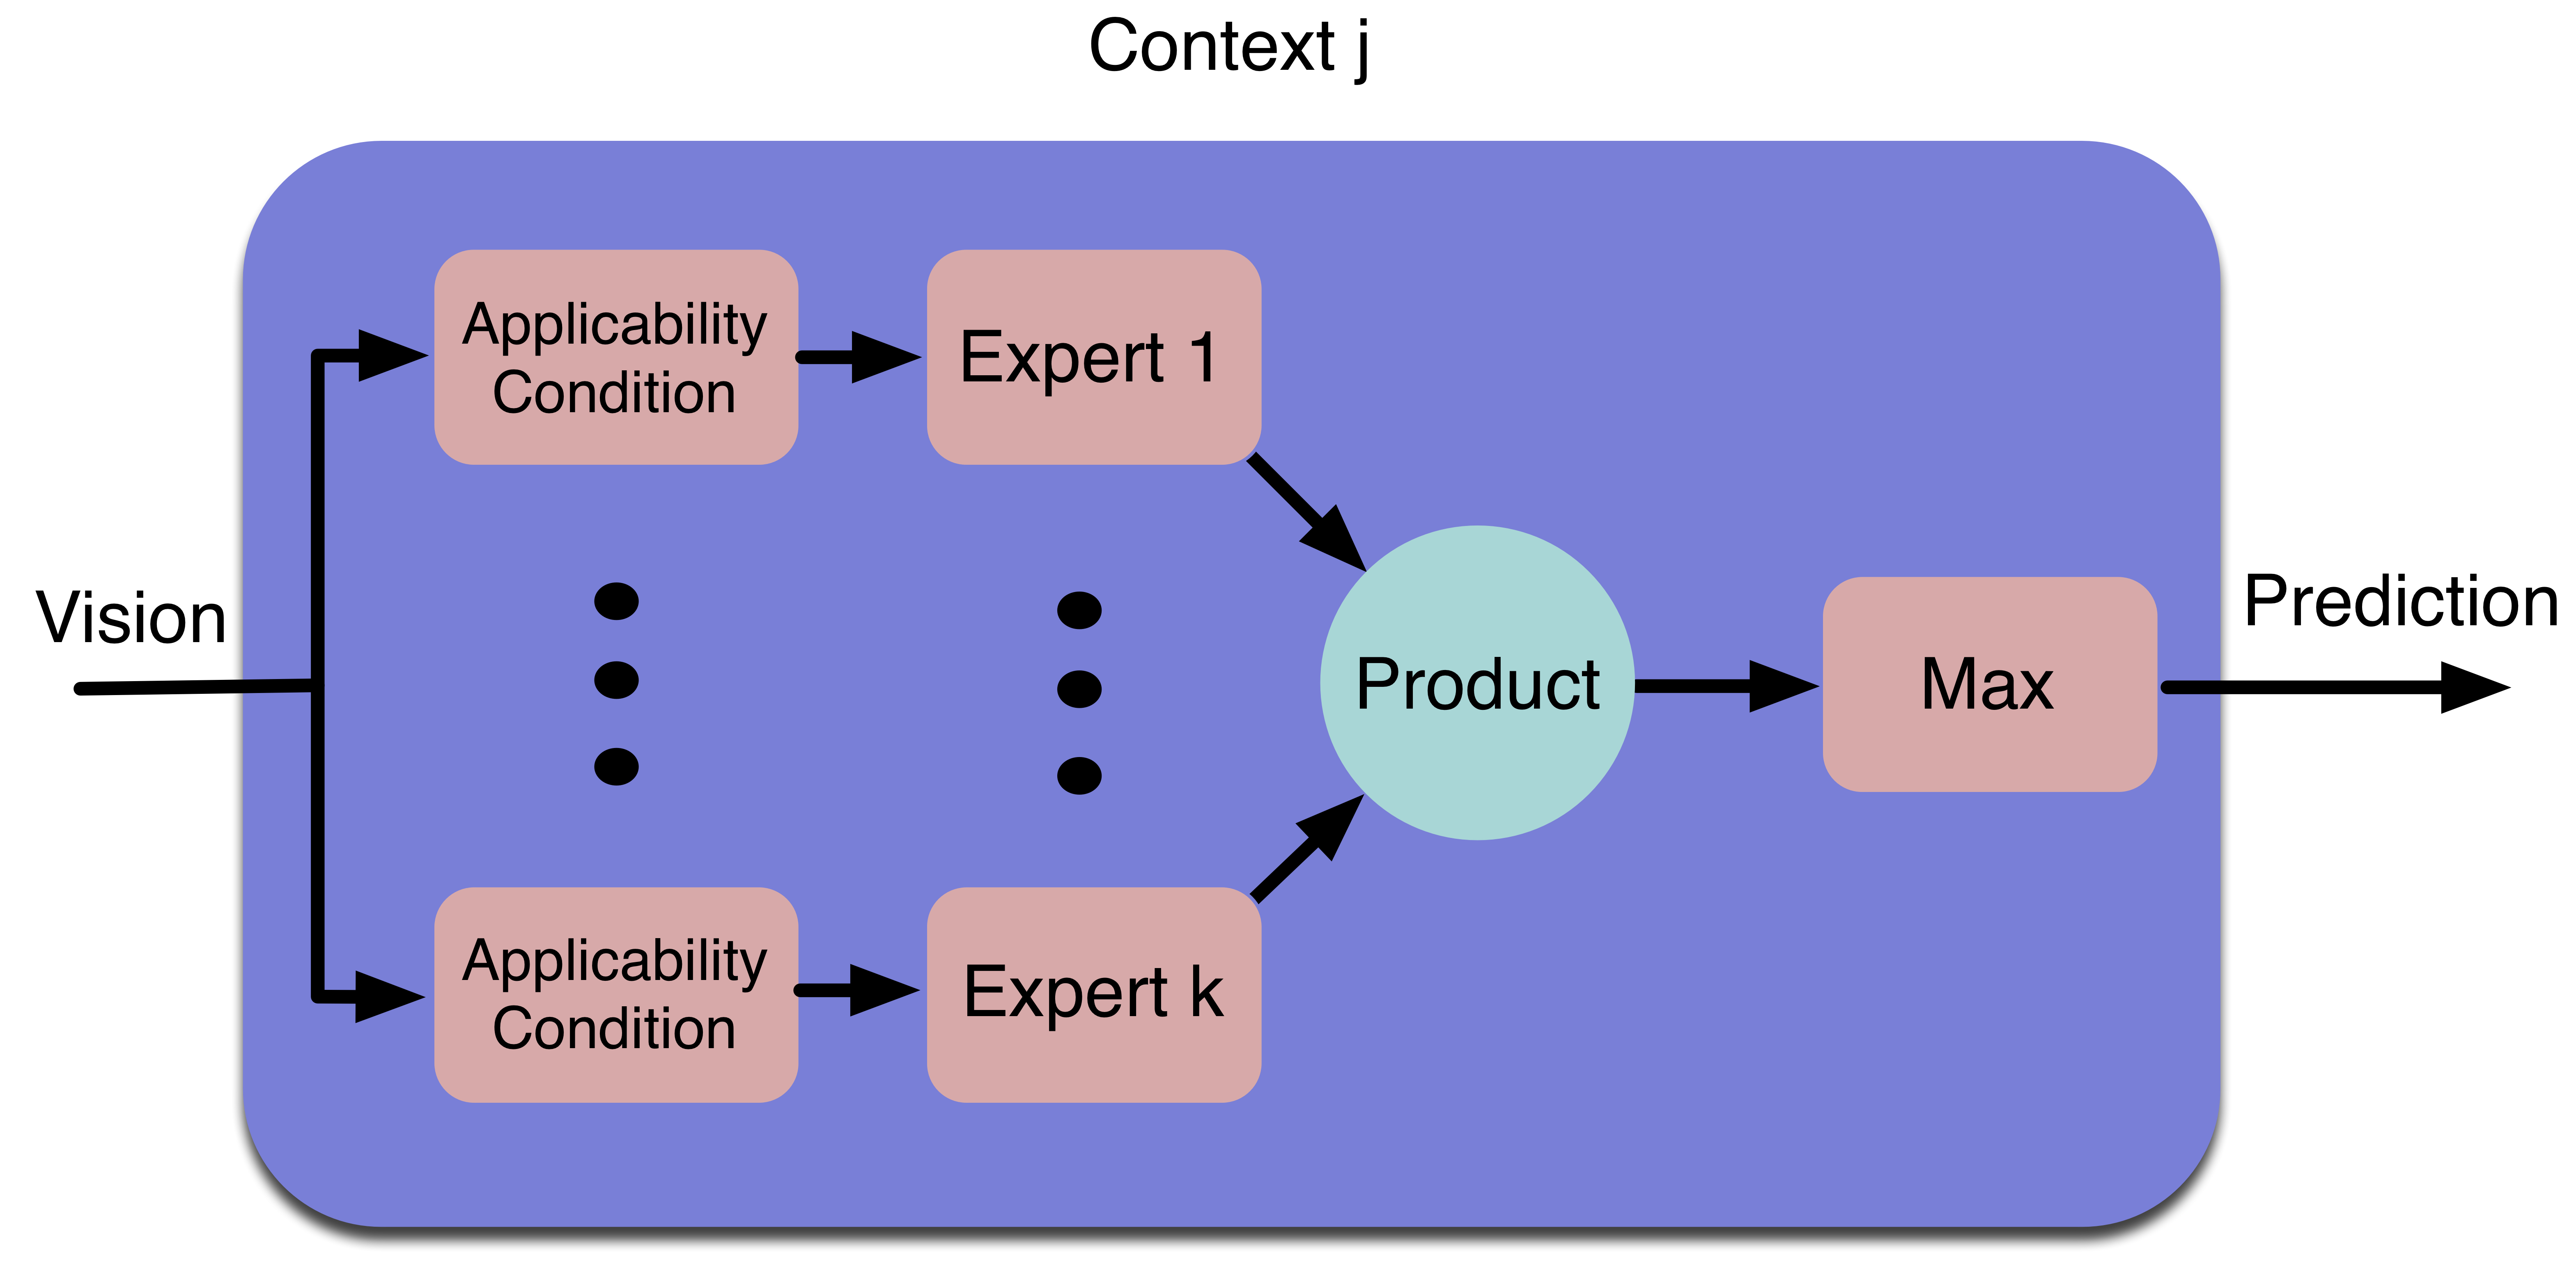
\includegraphics[width=0.85\columnwidth]{product-predictor}}
\caption[Factored Prediction]{ A Dynamic Product of Experts. This gives the structure of a factorised predictor for a single context as depicted in the modular learner in Figure~\ref{fig:three-prediction-problems}. Each expert in the product has an applicability condition which determines whether it contributes to the product. The applicable predictors combine densities over predictions to produce an overall density. This is optimised to produce a specific prediction.}
\label{fig:modular}
\end{figure}

The key property here is that the global, agent and environment densities encode different information about which rigid body transformations are feasible. By taking the product of these densities, only transformations which are feasible in all factors' frames will have high probability in the resulting combined distribution. In addition we make this product dynamic in the number of object-environment factors. Once the object surface is beyond some threshold distance from the environment surface its predictor switches off, and when it is close enough it switches on again. This enables us to keep only relevant predictors in the product at any one time -- improving prediction quality and efficiency. 

In summary we have now described two main formulations (regression and density estimation) able to incorporate varying amounts of information (G, G+A, G+A+E). We have also presented a reformulation of density estimation that factorises the prediction problem given information G+A or G+A+E into a product of experts. Which which information and problem formulation combine to provide the best prediction framework?
Is the factorised problem better able to exploit the additional
information than the unfactorised version? These questions can only be
answered using specific regression and density estimation
algorithms. Having completed our problem formulation we therefore now
turn to the details of the implementations we used for each framework.

\section{Implementation}\label{sec:Implementation}
for pushing
\newcommand{\bx}{\mathbf{x}}
\newcommand{\by}{\mathbf{y}}

%We have presented three formulations of prediction learning
%problems: i) as function approximation, ii) as density
%estimation and iii) as factored density estimation. 
%We have suggested that there may be an advantage to
%solving the density problem by factorising. We now detail the variety
%of parameterisations of rigid body transformations that may be
%employed, before describing the implementation details for our chosen
%regression and density estimation algorithms.
%\subsection{Parameterisation}\label{sec:Implementation.Parameterisation}
%

%%3-DOF 
%Positions can be parameterised uniquely by vectors $\mathbf{p} \in \mathbb{R}^3$, and
%3-DOF orientations by $3 \times 3$ rotation matrices $R \in SO(3)$
%which comprise the special orthogonal group $SO(3)$ with respect to matrix multiplication.
%There exist other parameterisations of $SO(3)$ which unlike rotation matrices
%may not be unique, but provide a lower-dimensional description
%of 3-DOF orientations.

%\subsubsection{Euler angles} $XYZ$ Euler angles $(\alpha, \beta, \gamma)$ describe rotation $R(\alpha, \beta, \gamma) \in SO(3)$ by combining elementary rotations about axes $X$, $Y$ and $Z$, by angle $\alpha$, $\beta$ and $\gamma$ respectively:
%\begin{equation}
%R(\alpha, \beta, \gamma) = R_Z(\gamma)R_Y(\beta)R_X(\alpha)
%\label{eq:Parameterisation.Euler}
%\end{equation}
%$XYZ$ Euler angles $(\alpha, \beta, \gamma)$ can be computed directly from coefficients of rotation matrix \eqref{eq:Parameterisation.Euler} as it is shown e.g. in \cite{murray_mathematical_1994}.

%Using Euler angles $(\alpha, \beta, \gamma) \equiv \boldsymbol{\phi}$,
%the parameterisation of a rigid-body transformation becomes
%$ \bx = [\, \mathbf{p}\, ;\, \boldsymbol{\phi}\, ] \in \mathbb{R}^6$.
%Euler angles, as a local parameterisation of $SO(3)$, suffer from singularities --
%there is no global invertible smooth mapping. % $(\alpha, \beta, \gamma) \rightarrow SO(3)$.
%Thus there can be two transformations that are arbitrarily close,
%but have a large difference in one of their Euler angles.
%This discontinuity places an extra burden on learning methods, which have to recover the circular
%nature of the Euler angle representation. However, if differences between angles are required
%(as e.g.\ for kernel density methods -- see Subsection~\ref{sec:Implementation.kde})
%then the problem can be finessed by computing a circular difference.
%
%%\subsubsection{Quaternions} Unit quaternions provide a global parameterisation of $SO(3)$, but at the cost of using four parameters instead of three as in the case of Euler angles. The unit quaternion $q$ is a normalised 4-dimensional vector associated with a rotation about unit-length axis $\omega \in \mathbb{R}^3$ by angle $\theta$:
%%
%%\begin{equation}
%%q = (\cos(\theta/2), \omega \sin(\theta/2))
%%\label{eq:Parameterisation.Quaternions.angleaxis}
%%\end{equation}
%
%If using quaternions, 
%the parameterisation of a rigid-body transformation becomes
%$ \bx = [\, \mathbf{p}\, ;\, \mathbf{q}\,] \in \mathbb{R}^7$,
%where  $\mathbf{q}$ is a unit quaternion.
%The set of all unit quaternions comprise a 3-dimensional sphere $S^3 \in \mathbb{R}^4$ and
%form a double cover of $SO(3)$, since a rotation about
%axis $\omega$ by angle $\theta$ is equivalent to a rotation about
%axis $-\omega$ by angle $-\theta$.
%Consequently any rotation $R \in SO(3)$ corresponds to exactly
%two quaternions $q$ and $-q$.
%Therefore any distance metric defined for quaternions $q$ and $q'$ must
%also test the case with $q$ and $-q'$.
The implementations are indexed by the algorithms used, and the information employed. For the function approximation formulation we used LWPR (Linear Weighted Projection Regression). For the unfactored density estimation formulation we used a variant of KDE (Kernel Density Estimation), and for the factored density estimation formulation we also used KDE, but denote it KDEF where -F denotes the use of factorisation. In addition, each algorithm: LWPR, KDE, KDEF, was implemented with differing amounts of input information. We denote these G (Global), GA (Global and Agent) and GAE (Global and Agent and Environment), as described previously. All the implementations depend on the parameterisation of rigid-body transformations chosen. In this paper we tested two parameterisations of orientation: Euler angles and quaternions (see e.g. \cite{murray_mathematical_1994}). We also employed two different densities for the quaternion parameterisation: Gaussian and von-Mises Fisher.

%%%%%%%%%%%%%%%%%%%%%%%%%%%%%%%%%%%%%%%%%%%%%%%%%%%%%%%%%%%%%%%%%%%%%%%%
\subsection{Regression method}\label{sec:Implementation.regression}

We used Locally Weighted Projection Regression (LWPR) \cite{vijayakumar_incremental_2005}, a powerful method applied widely in robotics, to estimate the mapping described by Equation~\eqref{eq:Learning.short}. The regression scheme was implemented using the LWPR software library \cite{klanke_library_2008}. LWPR was chosen because it employs an incremental learning algorithm that can handle a large number of input dimensions. After initial experimentation LWPR was run using the Euler angle parameterisation. 
%Several versions of the regression method were implemented, with varying amounts of information, corresponding to the global (referred to as LWPR-G), global and agent (LWPR-GA)
%%and global, agent and environment (LWPR-GAE) information.
%The Euler angle parameterisation was used for all the LWPR versions.
%In the case of LWPR-G, there were three rigid-body transformations provided as inputs to LWPR, which formed an 18-dimensional input space. The output was encoded as a 6-dimensional vector, that described the motion of the object $T^{B_{t}, B_{t+1}}$.
%For the case of the global plus agent information
%For LWPR-GA, the input space was augmented by 6 dimensions to accommodate the transformation $T^{A^{l}_t, B^{l}_t}$.
%The contextual information provided by the agent contact
%can be characterised as discrete,
%since the agent contact only acts when the finger and object are touching,
%i.e.\ for a discrete set of values in the input space.
%This is challenging for LWPR,
%which is better suited to operating with continuous contexts.
%For LWPR-GA and LWPR-GAE, the extension of the output space (to 12 dimensions) with $T^{B^{l}_{t}, B^{l}_{t+1}}$ did not change the prediction of $T^{B_{t}, B_{t+1}}$, since LWPR treats each output dimension independently as stated in \cite{klanke_library_2008}.
%Thus, it was not possible to take advantage of the extra information provided by $T^{B^{l}_{t}, B^{l}_{t+1}}$ in the same manner
%as the density estimation approach (Equation~\eqref{eq:Learning.densitylocal}).
%
%Finally, when using (possibly several) environment contacts, the input space was again enlarged, to form domains of up to 42 dimensions.
%In this formulation of regression, the inputs from the global, agent and environment frames were treated uniformly, whereas the density estimation scheme of Equation~\eqref{eq:Learning.MultiFactorProduct}
%made a clear distinction between these three types of input.
%Furthermore, as there is no special structure, such as a factored density, in our regression framework, we may expect
%poor performance when extrapolating to novel actions and object shapes. 
The dimensions of the input and output spaces of each LWPR predictor are summarised in Table~\ref{tab:InpOutSpaceLWPR}.

\begin{table}[b]
\begin{center}
\begin{tabular}{|l|l|l|}
\cline{1-3}
Predictor & input space & output space \\
\cline{1-3}
LWPR-G euler & 18 & 6 \\
LWPR-GA euler & 24 & 6 \\
LWPR-GAE euler & 24 + N*6 & 6 \\
\cline{1-3}
\end{tabular}
\end{center}
\caption[Input/output space LWPR]{Dimensions of input and output spaces
of LWPR predictors, where $N$ is the number of
"environment contacts".}\label{tab:InpOutSpaceLWPR}
\end{table}


%%%%%%%%%%%%%%%%%%%%%%%%%%%%%%%%%%%%%%%%%%%%%%%%%%%%%%%%%%%%%%%%%%%%%%%%
\subsection{Kernel density method}\label{sec:Implementation.kde}

A variant of Kernel Density Estimation (KDE) \cite{scott2004multi-dimensional} is used to approximate the conditional densities employed in the product in Equation~\eqref{eq:Learning.MultiFactorProduct}.
%KDE is an example of a non-parametric method,
%where an underlying distribution is modelled by a mixture
%of $N$ identical kernels centred on \textit{training samples}.
%We shall use ``KDEF" to denote the KDE algorithm applied to the factored density \eqref{eq:Learning.MultiFactorProduct}, and use ``KDE" to label the unfactored case~\eqref{eq:Learning.density}.
%There are three variants of KDEF: KDEF-G, KDEF-GA and KDEF-GAE,
%where the suffix denotes whether information from agent~(A)
%and environment~(E) contacts is utilised, in addition to global (G) information.

%Training samples are composed of $D = D^x + D^y$ rigid body transformations,
%where $D$, $D^x$ and $D^y$ are the numbers of transformations
%comprising the joint, conditioning and conditioned densities respectively.
%For example, $D^y$ equals one for all conditional distributions
%in product \eqref{eq:Learning.MultiFactorProduct},
%however $D^x$ equals three for global joint distribution
%\eqref{eq:Learning.densityglobal}, two for local joint distribution
%\eqref{eq:Learning.densitylocal} and one for local contact joint
%distributions \eqref{eq:Learning.densityenv}.
%
%The stacked parameters of conditional distributions
%are denoted by (italic) $T^x$ and $T^y$:
%\begin{subequations}
%\label{eq:Density.Estimation.transformations}
%\begin{align}
%T^x &= \left\{T_1, \ldots, T_{D^x}\right\} \\
%T^y &= \left\{T_1, \ldots, T_{D^y}\right\}
%\end{align}
%\end{subequations}
%Transformations $T^x$ and $T^y$ are then mapped onto parameter vectors
%using one of the parameterisations introduced in
%Subsection~\ref{sec:Implementation.Parameterisation}:
%\begin{subequations}
%\label{eq:Density.Estimation.sample}
%\begin{align}
%x(T^x) &= \left[\begin{array}{ccc}x_1(T^x_1) & \ldots & x_{D^x}(T^x_{D^x}) \end{array}\right]^\mathrm{T} \\
%y(T^y) &= \left[\begin{array}{ccc}y_1(T^y_1) & \ldots & y_{D^y}(T^y_{D^y}) \end{array}\right]^\mathrm{T}
%\end{align}
%\end{subequations}
%\noindent where (non-italic) $\mathrm{T}$ denotes the
%vector transpose operation and where each $i$-th
%rigid body transformation $T^x_i$ and $T^y_i$ is parameterised
%by vectors $x_i$ and $y_i$ respectively:
%\begin{subequations}
%\label{eq:Density.Estimation.sampleblock}
%\begin{align}
%x_i(T^x_i) &= \left[\begin{array}{cc}x^l_i & x^o_i\end{array}\right]^\mathrm{T} \\
%y_i(T^y_i) &= \left[\begin{array}{cc}y^l_i & y^o_i\end{array}\right]^\mathrm{T}
%\end{align}
%\end{subequations}
%\noindent with location vectors $x^l_i, y^l_i \in \mathbb{R}^3$ and
%orientation vectors $x^o_i, y^o_i \in \mathbb{R}^3$ for Euler angles
%or $x^o_i, y^o_i \in \mathbb{R}^4$ for quaternions.

%A product of $N$ factors \eqref{eq:Learning.MultiFactorProduct}
%for transformations $T^y$ given $T^x$ can be written as:
%\begin{equation}
%p(T^y|T^x) = C \mathop{\prod}_{i=1 \ldots N} p_i(y(G_i^{-1} T^y G_i)|x(G_i^{-1} T^y G_i))
%\label{eq:Density.Estimation.product}
%\end{equation}
%\noindent where $C$ is a normalisation constant,
%$p_i$ are single factor conditional densities,
%and $G_i^{-1} T^x G_i$ and $G_i^{-1} T^y G_i$ are ``block''
%similarity transformations such that
%$(T_{body}^x)_j = G_i^{-1} (T_{in}^x)_j G_i$ and
%$(T_{body}^y)_j = G_i^{-1} (T_{in}^y)_j G_i$ where
%$G_i$ is an instantaneous frame of the $i$-th factor
%(also see \eqref{eq:Learning.Body1}).

The conditional probability density (CPD) $p_{qs}$ in Equation~\eqref{eq:Learning.density} and each CPD or factor in
Equations~\eqref{eq:Learning.densityglobal} to~\eqref{eq:Learning.densityenv}
can be represented (up to a normalisation constant) as a mixture of products of simple kernels:
\begin{equation}
P(\mathbf{Y}|\mathbf{X}) \propto
\mathop{\sum}_{j=1 \ldots M}
K(\mathbf{X}, \hat{\mathbf{X}}_j, H \mathbf{h}^{(X)})
K(\mathbf{Y}, \hat{\mathbf{Y}}_j, H \mathbf{h}^{(Y)})
\label{eq:Density.Estimation.mixture}
\end{equation}
\noindent where the vector $\mathbf{X}$ corresponds to the parameters of the transformations associated with the conditioning variables of the CPD, and the components of vector $\mathbf{Y}$ parameterise the transformation representing the predicted object motion. During learning, for each of the $M$ training samples,
a pair of vectors $\hat{\mathbf{X}}_j$ and $\hat{\mathbf{Y}}_j$
is constructed from the parameter values of the associated transformations. These vectors then remain fixed during prediction.
Vectors $\mathbf{h}^{(X)}$ and $\mathbf{h}^{(Y)}$, known as \textit{bandwidths}, are then estimated from training samples using
the ``multivariate rule-of-thumb'' \cite{scott2004multi-dimensional}.
These bandwidth parameters $\mathbf{h}^{(X)}$ and $\mathbf{h}^{(Y)}$ are additionally multiplied by a meta-parameter $H \in \mathbb{R}$ which can be estimated by a model selection process (see Subsection~\ref{sec:Experiment.Setup}). Note that $H$, $\mathbf{h}^{(X)}$, $\mathbf{h}^{(Y)}$, $\hat{\mathbf{X}}_j$
and $\hat{\mathbf{Y}}_j$ will depend on the particular CPD to be estimated. (If needed, this dependency will be made explicit in the sequel, by using an extra index $k$.)

Each kernel function $K()$ in Equation~\eqref{eq:Density.Estimation.mixture} can be written in the form:
\begin{equation}
K(\mathbf{X}, \hat{\mathbf{X}}, \mathbf{h}) =
\mathop{\prod}_{l=1 \ldots L} \exp \left[-\frac{1}{2}d(\bx_l, \hat{\bx}_l, \mathbf{h}_l)\right]
\label{eq:Density.Estimation.kernel}
\end{equation}
\noindent where the $\bx_l$ are the parameters of the $L$ transformations that are the conditioning variables in the CPD. A similar form exists for $\mathbf{Y}$, with $L=1$. Furthermore $d()$ is a \textit{distance function} that determines the kernel type. We employed Gaussian kernels for both Euler and quaternion representations, and additionally Gaussian+Von Mises Fisher kernels for the case of quaternions.
\begin{enumerate}
\item For a \textit{Gaussian kernel}:
\begin{equation}
d_\mathrm{Gauss}(\bx, \hat{\bx}, \mathbf{h}) =
(\bx - \hat{\bx})^\mathrm{T}\mathbf{C}^{-1}(\bx - \hat{\bx})
%\mathop{\sum}_{i=1 \ldots \mathrm{DIM}(x)} \left(\frac{x_i - \hat{x}_i}{h_i}\right)^2
\label{eq:Density.Estimation.gaussiandist}
\end{equation}
\noindent corresponding to a Mahalanobis distance with diagonal covariance
$\mathbf{C}_{ii} = [\mathbf{h}]_i$.
Here $\bx, \hat{\bx}, \mathbf{h}$ are in $\mathbb{R}^6$ for Euler angles or $\mathbb{R}^7$ for the quaternion parameterisation.
%\begin{equation}
%d_\mathrm{Mahalanobis}(\bx, \hat{\bx}, \mathbf{C}) = (x - \hat{x})^\mathrm{T}\mathbf{C}^{-1}(x - \hat{x})
%\label{eq:Density.Estimation.Mahalanobis}
%\end{equation}
\item For a product of a Gaussian kernel and \textit{von~Mises--Fisher} kernel:
\begin{multline}
d_\mathrm{GaussVMF}(\bx, \hat{\bx}, \mathbf{h}) =
d_\mathrm{Gauss}(\mathbf{p}, \hat{\mathbf{p}}, \mathbf{h}^{(p)}) \; +\\
d_\mathrm{VMF}(\mathbf{q}, \hat{\mathbf{q}}, h^{(q)})
\label{eq:Density.Estimation.gaussvmfdist}
\end{multline}
\noindent where %$\mathbf{p} \in \mathbb{R}^3$,
$\mathbf{h} = \left[ \mathbf{h}^{(p)} ; h^{(q)} \right]$,
$\mathbf{h}^{(p)} \in \mathbb{R}^3$,
$h^{(q)} \in \mathbb{R}$,
%$h = \left[\begin{array}{cc}h^l & h^o\end{array}\right]^\mathrm{T}$, $h^o \in \mathbb{R}$,
and (see e.g.\ \cite{abramowitz_handbook_1965}):
\begin{equation}
d_\mathrm{VMF}(\mathbf{q}, \hat{\mathbf{q}}, h^{(q)}) =
2 h^{(q)} \left(1 - \left| \mathbf{q} . \hat{\mathbf{q}} \right|\right)
\label{eq:Density.Estimation.vmfdist}
\end{equation}
\noindent where $\mathbf{q} . \hat{\mathbf{q}}$ is the quaternion dot product and taking the absolute value fixes the double cover problem.
\end{enumerate}

The Von Mises--Fisher kernel \eqref{eq:Density.Estimation.kernel} with \eqref{eq:Density.Estimation.vmfdist} is an approximation (up to a multiplicative constant \cite{detry_learning_2010}) of the von~Mises--Fisher distribution:
\begin{equation}
f_4(x, \mu, \kappa) = C_4(\kappa)\exp(\kappa x^\mathrm{T} \mu)
\label{eq:Density.Estimation.vmf}
\end{equation}
\noindent where $C_4(\kappa)$ is a normalisation constant and where $\mu$ and $\kappa$ are unit quaternions. In directional statistics $f_4(x,\mu,\kappa)$ is a probability distribution on $S^3 \in \mathbb{R}^4$ with mean $\mu$ and dispersion parameter $\kappa$.

The dimensions of the input $\mathbf{X}$ and output $\mathbf{Y}$ spaces for KDEF predictors are summarised in Table~\ref{tab:InpOutSpaceKDE}.

\begin{table}[b]
\begin{center}
\begin{tabular}{|l|l|l|l|l|}
\cline{1-5}
Predictor & \multicolumn{3}{|c|}{input space} & output space \\
\cline{2-4}
 & global & agent & env & \\
\cline{1-5}
KDEF euler & 18 & 12 & 6 & 6 \\
KDEF quat & 21 & 14 & 7 & 7 \\
KDEF vmf & 21 & 14 & 7 & 7 \\
\cline{1-5}
\end{tabular}
\end{center}
\caption[Input/output space KDEF]{Input and output space dimensions of KDEF factors.}\label{tab:InpOutSpaceKDE}
\end{table}

Following Equation~\eqref{eq:Learning.MultiFactorProduct},
the prediction problem at each step can be defined as finding that
transformation $\widetilde{T}^y$ which maximises the product of conditional densities
\eqref{eq:Learning.product} given fixed $T^x$, i.e.:
\begin{equation}
\widetilde{T}^y = \argmax{T^y} p(T^y|T^x)
\label{eq:Density.Estimation.max}
\end{equation}
Prior to the maximisation procedure, for each factor $k$
and each training sample $j$ values of 
$K(\mathbf{X}, \hat{\mathbf{X}}_j, H \mathbf{h}^{(X)})$
in \eqref{eq:Density.Estimation.mixture} are computed and assigned
to $w_{k,j}$, referred to as \textit{weights}.
The normalised weight $w_{k,j}$ can be interpreted as a probability of
generating $\mathbf{X}$ from a multivariate Gaussian centred at $\hat{\mathbf{X}}_{j,k}$
with covariance $\mathbf{C}_{ii} = [H_k \mathbf{h}^{(X)}_k]_i$.
In order to increase the computational efficiency of the optimisation procedure
we only consider the $M^{max}_k < M_k$ most relevant training samples,
(i.e. those with the highest weights $w_{k,j}$ at the query point $\mathbf{X}$).
These are identified by calculating, for each training sample, the value
of the distance function $d()$ (from Equation~\eqref{eq:Density.Estimation.kernel}).
The training samples are then sorted according to the distance using a
partial sort algorithm (e.g. \cite{knuth_searching_1998})
to identify the $M^{max}_k$ most relevant training samples.

Equation~\eqref{eq:Density.Estimation.max} is computed using the
differential evolution (DE) optimisation algorithm \cite{storn_differential_1997}.
Note that one cannot use the mean-shift algorithm \cite{cheng_mean_1995}
mostly due to the product involved in \eqref{eq:Density.Estimation.max}.
DE is particularly simple to tune, since it is controlled by only
two meta-parameters: a \textit{crossover probability}
and a \textit{population size} of candidate solutions.
If the number of generations is fixed,
the total run time scales linearly with the number of factors,
their dimensionality and the number samples.
Optionally, the entire maximisation procedure is stopped when
no further significant improvement is observed.
The optimisation algorithm requires an ability to sample from the
product~\eqref{eq:Learning.product}.
This can be achieved by performing the following two step procedure:

\begin{enumerate}
\item Randomly choose an factor $k$ and then sample $j$ from
a set of samples $\{w_{k,j}\}$ using the importance sampling algorithm
with importance weights $w_{k,j}$ (e.g. \cite{bishop_pattern_2006}).
\item Sample from a multivariate Gaussian centred at $\hat{\mathbf{Y}}_{j,k}$ with
covariance $\mathbf{C}_{ii} = [H_k \mathbf{h}^{(Y)}_k]_i$, using
e.g.\ the Marsaglia polar method \cite{marsaglia_convenient_1964}.
\end{enumerate}

Importantly, after generating a new solution candidate,
all sub-vectors $\mathbf{q}$ have to be normalised when a quaternion parameterisation is used.

%All KDEF factors are assumed to be independent,
%therefore their domains do not sum up.

To improve the efficiency of the implementation, no learning or prediction
was performed in a given trial until the initial contact was made between
robotic finger and object. This procedure was employed by
the KDE, KDEF and LWPR predictors. This means that the learners and
predictors are switched on by an initial finger-object contact.
In addition, for the KDEF predictor, at each time step,
agent and environment factors were only used
if the corresponding agent-object or object-environment distance
was within a certain threshold. 
% LWPR can't do this switching off/on of contacts

%%%%%%%%%%%%%%%%%%%%%%%%%%%%%%%%%%%%%%%%%%%%%%%%%%%%%%%%%%%%%%%%%%%%%%%

\newlength{\barchartwidth}
\setlength{\barchartwidth}{6.5cm}

%%%%%%%%%%%%%%%%%%%%%%%%%%%%%%%%%%%%%%%%%%%%%%%%%%%%%%%%%%%%%%%%%%%%%%%
\section{Experimental study}\label{sec:Experiment}

%%%%%%%%%%%%%%%%%%%%%%%%%%%%%%%%%%%%%%%%%%%%%%%%%%%%%%%%%%%%%%%%%%%%%%%
\subsection{Overview of experiments}\label{sec:Experiment.Overview}

We conducted three experiments, one for each problem in Section~\ref{sec:schema}: P1 (action interpolation), P2 (action transfer) and P3
(shape transfer). Each experiment tests all combinations of information (G,A,E) and learning algorithm (LWPR, KDE, KDEF) (see Table~\ref{tab:algs}). The structure of these experiments reflects the structure of our hypotheses: H1-H3.

{\bf Experiment P1 (action interpolation):} tests hypothesis. {\em {\bf H1}: a modular learning approach can outperform physics engines for prediction of rigid body motion.} Each learning method was used to learn a context/object specific predictor and the results were compared to the predictions of a physics simulator that had also been tuned to each object in a modular manner. We also compared the effects of different parameterisations of rigid body transformations.

{\bf Experiment P2 (action transfer):} tests hypothesis {\em {\bf H2}: learned predictions can be transferred to novel actions.} The learners were trained with a reduced action set on a non-symmetric object and then tested on that object with novel actions. We performed this in simulation and with a real object.

{\bf Experiment P3 (shape transfer):} tests hypothesis {\em {\bf H3}: learned predictions can be transferred to novel shapes.} Learners were trained on one or more objects, and tested on an object of different shape. Transfer was tested both in simulation and with real objects.

\subsection{Experimental setup}\label{sec:Experiment.Setup}

In each trial the robot finger moved in a straight line, pushing
an object for 10 seconds, making contact at a randomly selected point
on its surface (Figure~\ref{fig:Setup}). Video and finger position were captured at 30Hz, including a 1 second buffer at either end of the finger trajectory. Learning used the pose of the object in every other frame estimated using a particle filter tracker \cite{morwald_edge_2009}. For test trials the trajectory of the finger was known a priori and the object pose observed only at the initial frame. Using these a trajectory was predicted for the object over 150 steps (10 seconds). The predicted trajectory was created purely using the forward model and did not use any observations during the push to update its prediction. For real experiments, a 5-axis robot arm with a single finger was used. Simulation experiments used the NVIDIA PhysX engine to provide ground-truth. The PhysX engine was evaluated as a predictor itself in real object trials.

\begin{figure}[t]
\centerline{
%\includegraphics[width=4.3cm]{topple1}
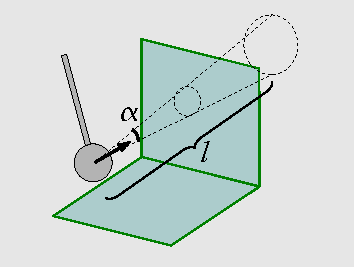
\includegraphics[width=3.2cm]{training}
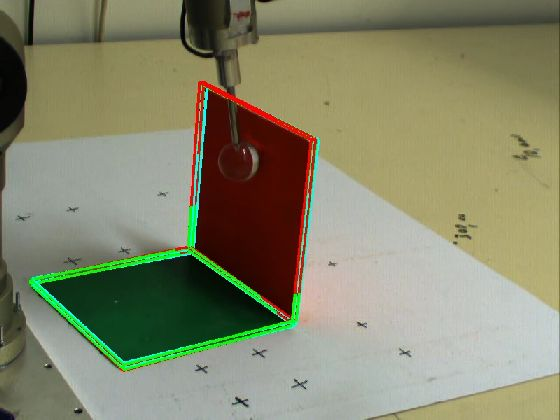
\includegraphics[width=3.2cm]{complex1}
}
\centerline{
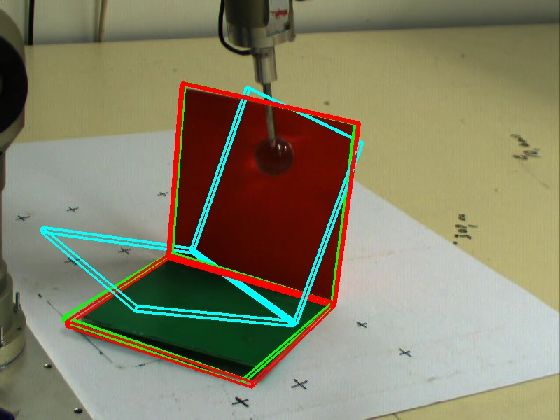
\includegraphics[width=3.2cm]{complex2}
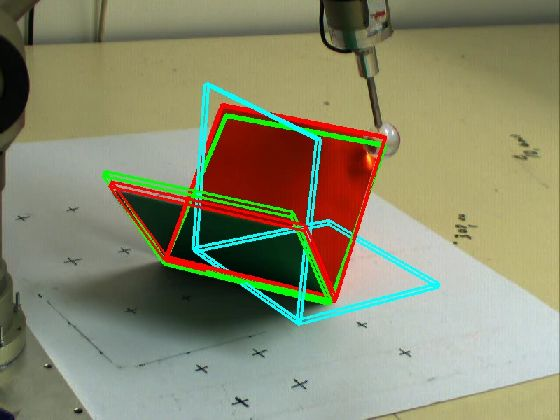
\includegraphics[width=3.2cm]{complex4}
}
\caption[Setup]{
A robot finger pushes in a straight-line of length $l$=25$\pm$5 cm within a cone of angle $\alpha$=20 deg toward an object (top left). The start point is randomised so that each region on the vertical face is equally likely to be pushed. The red wire-frame shows the output of the visual tracker, the green wire-frame the object pose predicted by the KDEF learner, and the blue wire-frame the prediction of the PhysX simulator, which is plausible but inaccurate.}
\label{fig:Setup}
\end{figure}

Local frames for environment contacts in the -GAE variants were fixed
by hand to the edges of objects. In test cases with new objects the
frames were again fixed by hand.  An item for future work is to
perform this process automatically.  All methods required parameter tuning. Model selection was performed in experiment P1 to establish reasonable parameter values, which were then used in experiments P2 and P3.  It was not possible to perform fully systematic optimisations for LWPR, KDE and KDEF due to the size of the parameter spaces.  Rather, subsets of the parameter space were selected by inspection and then explored using grid search.  Models were evaluated on a separate hold-out set, of the same size as the test set. Model selection by full grid search was performed for the following parameters of the PhysX simulator: static friction, dynamic friction and the coefficient of restitution. PhysX has access to full mesh and contact information. In addition to model selection the three different parameterisations (Gauss-Euler, Gauss-Quaternion, Von-Mises-Fisher-Quat) of rotations for the density estimation method were studied in experiment P1, and subsequently the best solution was used in experiments P2 and P3. For LWPR we used the Euler parameterisation throughout experiments P1, P2 and P3. For experiment P1 we performed 10-fold cross-validation. The sizes of the training and test sets are stated in the method for each experiment. For transfer learning experiments P2 and P3, disjoint training and test sets were used. For clarity a complete set of acronyms for the algorithm-information combinations is given in Table~\ref{tab:algs}. 

\begin{table}[b]
\begin{center}
\begin{tabular}{|l|l|l|l|}\hline
 & \multicolumn{3}{|c|}{Information} \\ \hline
Predictor & G & G+A & G+A+E \\ \hline
LWPR & LWPR-G& LWPR-GA & LWPR-GAE \\ \hline
KDE & KDE-G & KDE-GA & KDE-GAE \\ \hline
KDEF & KDEF-G & KDEF-GA & KDEF-GAE \\ \hline
PhysX & n/a & n/a & n/a \\ \hline
\end{tabular}
\end{center}
\caption{Algorithm-information variants.}
\label{tab:algs}
\end{table}

%%%%%%%%%%%%%%%%%%%%%%%%%%%%%%%%%%%%%%%%%%%%%%%%%%%%%%%%%%%%%%%%%%%%%%%

\subsection{Performance measure}\label{sec:Experiment.Performance}

In all experiments with real objects, predicted trajectories were evaluated against the visual tracked object pose. The tracker does not provide perfect ground-truth, yielding errors of $\pm$2mm. Prediction performance is evaluated as follows.

At any particular time step, $t$, a large number, $N$, of randomly chosen points $p_{n}^{1,t}$, where $n=1 \ldots N$, are rigidly attached to an object at the ground-truth pose, and the corresponding points $p_{n}^{2,t}$ to an object at the predicted pose. At time step $t$, an average error $E_t$ can now be defined as the mean of displacements between points on the object at the predicted pose and points on the object at the ground-truth pose:
\begin{equation}
E_t = \frac{1}{N} \mathop{\sum}_{n=1 \ldots N}|p_{n}^{2,t}-p_{n}^{1,t}|
\label{eq:defn_Rt}
\end{equation}
Note that for each push action, we predict approximately 150
consecutive steps into the future, with no recursive filtering or
corrector steps, hence it is expected that errors will grow with range
from the initial object pose. We therefore find it more meaningful to
normalise all errors with respect to an ``average range'', $R_t$, of
the object from its starting position, defined as:
\begin{equation}
R_t = \frac{1}{N} \mathop{\sum}_{n=1 \ldots N}|p_{n}^{1,t}-p_{n}^{1,0}|
\label{eq:defn_Et}
\end{equation}
For a test data set, consisting of $K$ robotic pushes, each of which breaks down into many consecutive predictions over $T$ time steps, we can now define average error and normalised average error. Note that the normalised error measure necessarily has no units.
\begin{align}
E_{av} &= \frac{1}{K} \mathop{\sum}_{k=1}^{K} \frac{1}{T} \mathop{\sum}_{t=1}^{T} E_t,
&E_{av}^{norm} &= \frac{1}{K} \mathop{\sum}_{k=1}^{K} \frac{1}{T} \mathop{\sum}_{t=1}^{T} \frac{E_t}{R_t}
\label{eq:Error1}
\end{align}


\begin{figure}[t]
\centerline{
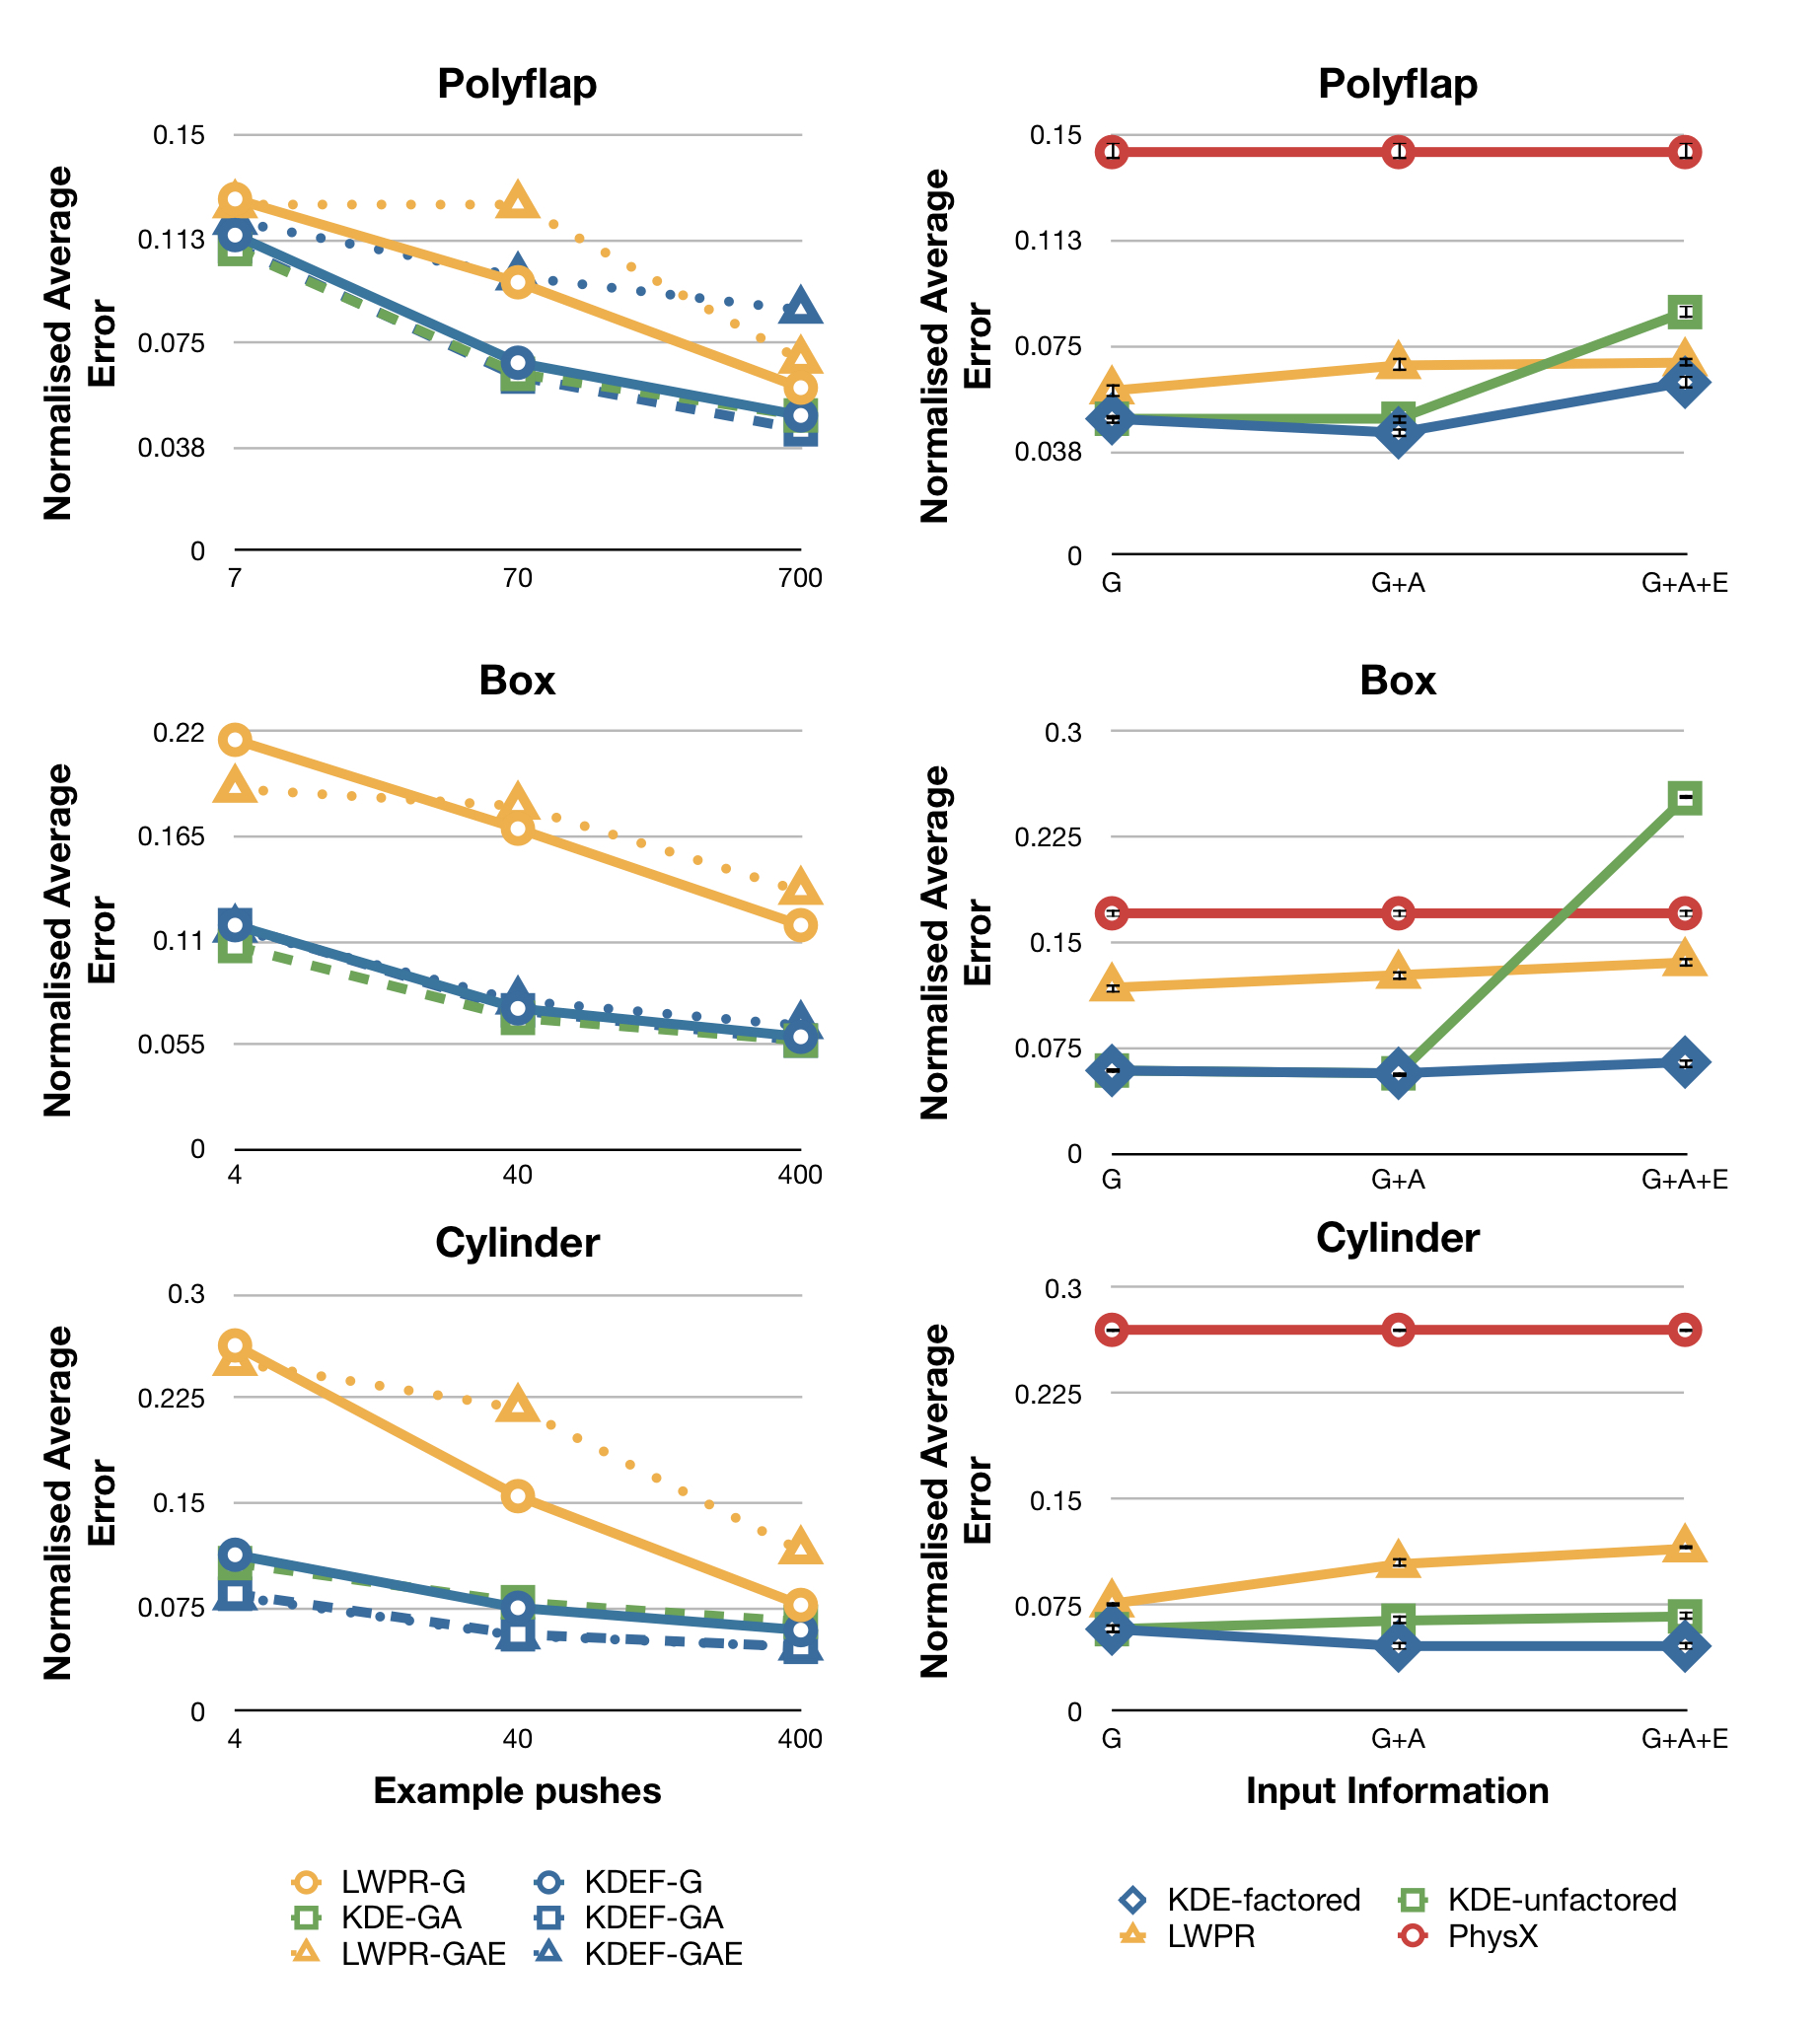
\includegraphics[width=\columnwidth]{graphs_jw/P1-graphs}
%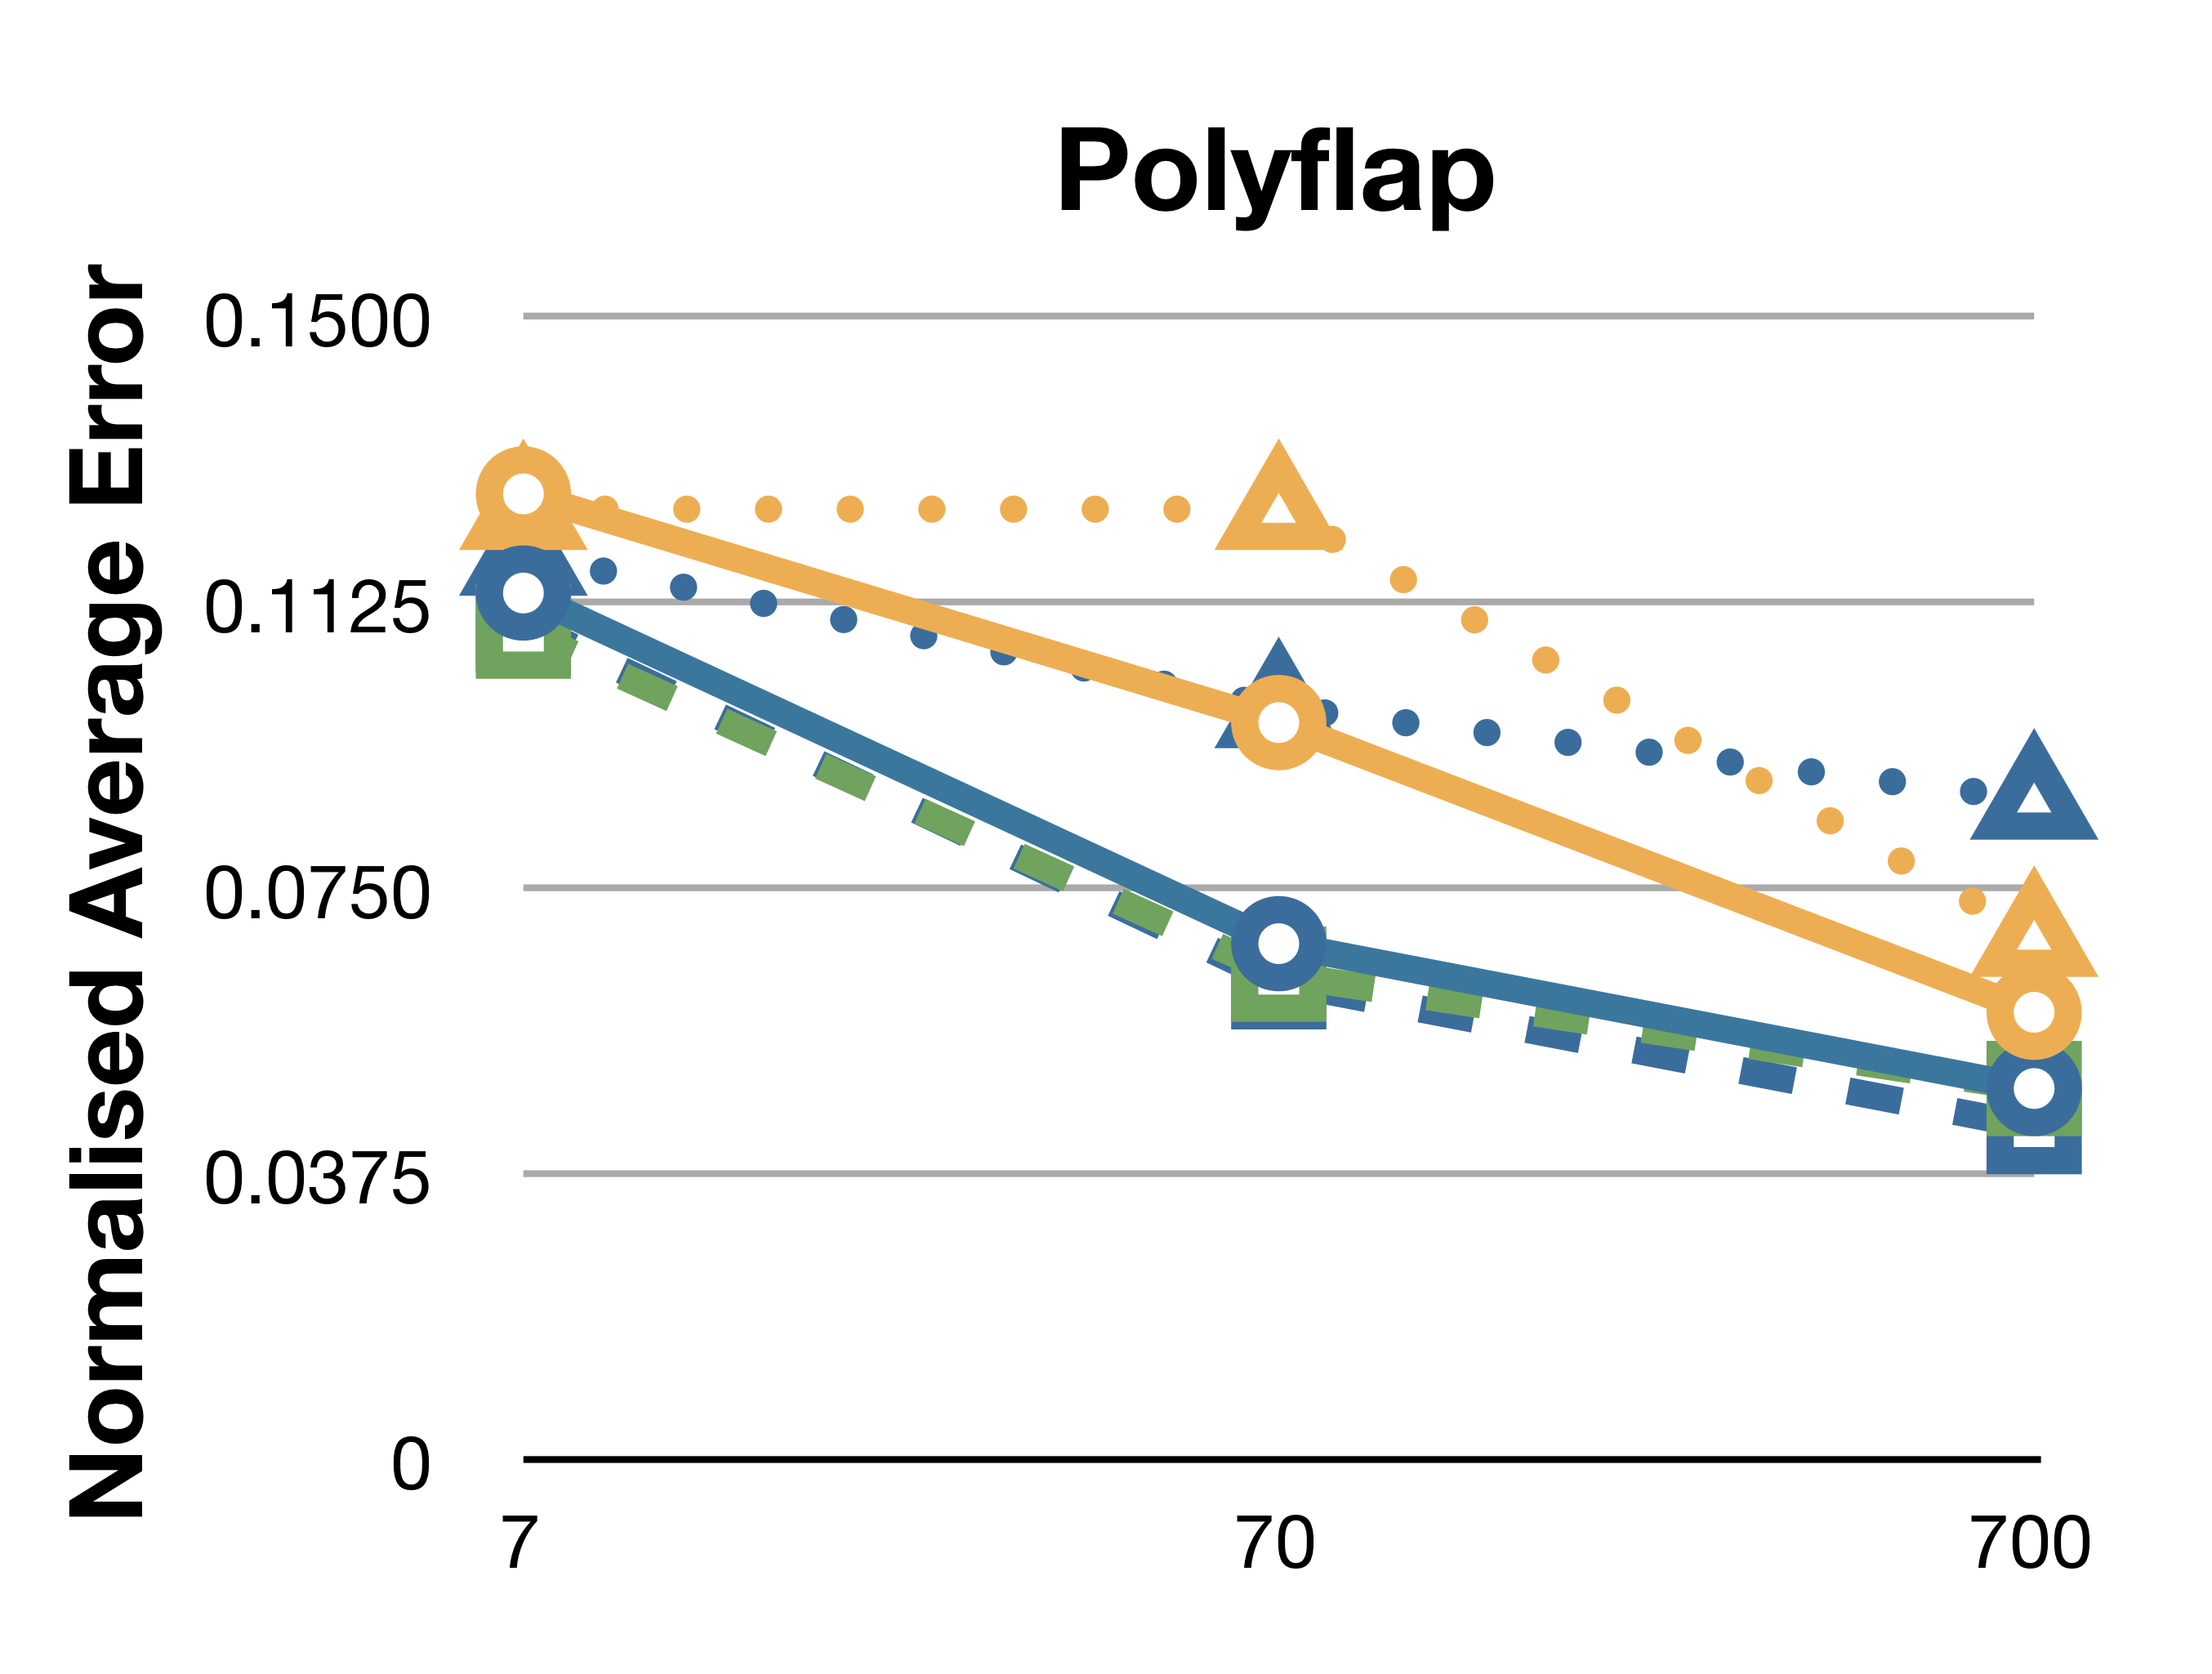
\includegraphics[width=0.45\columnwidth]{graphs_jw/L1av_graph}
%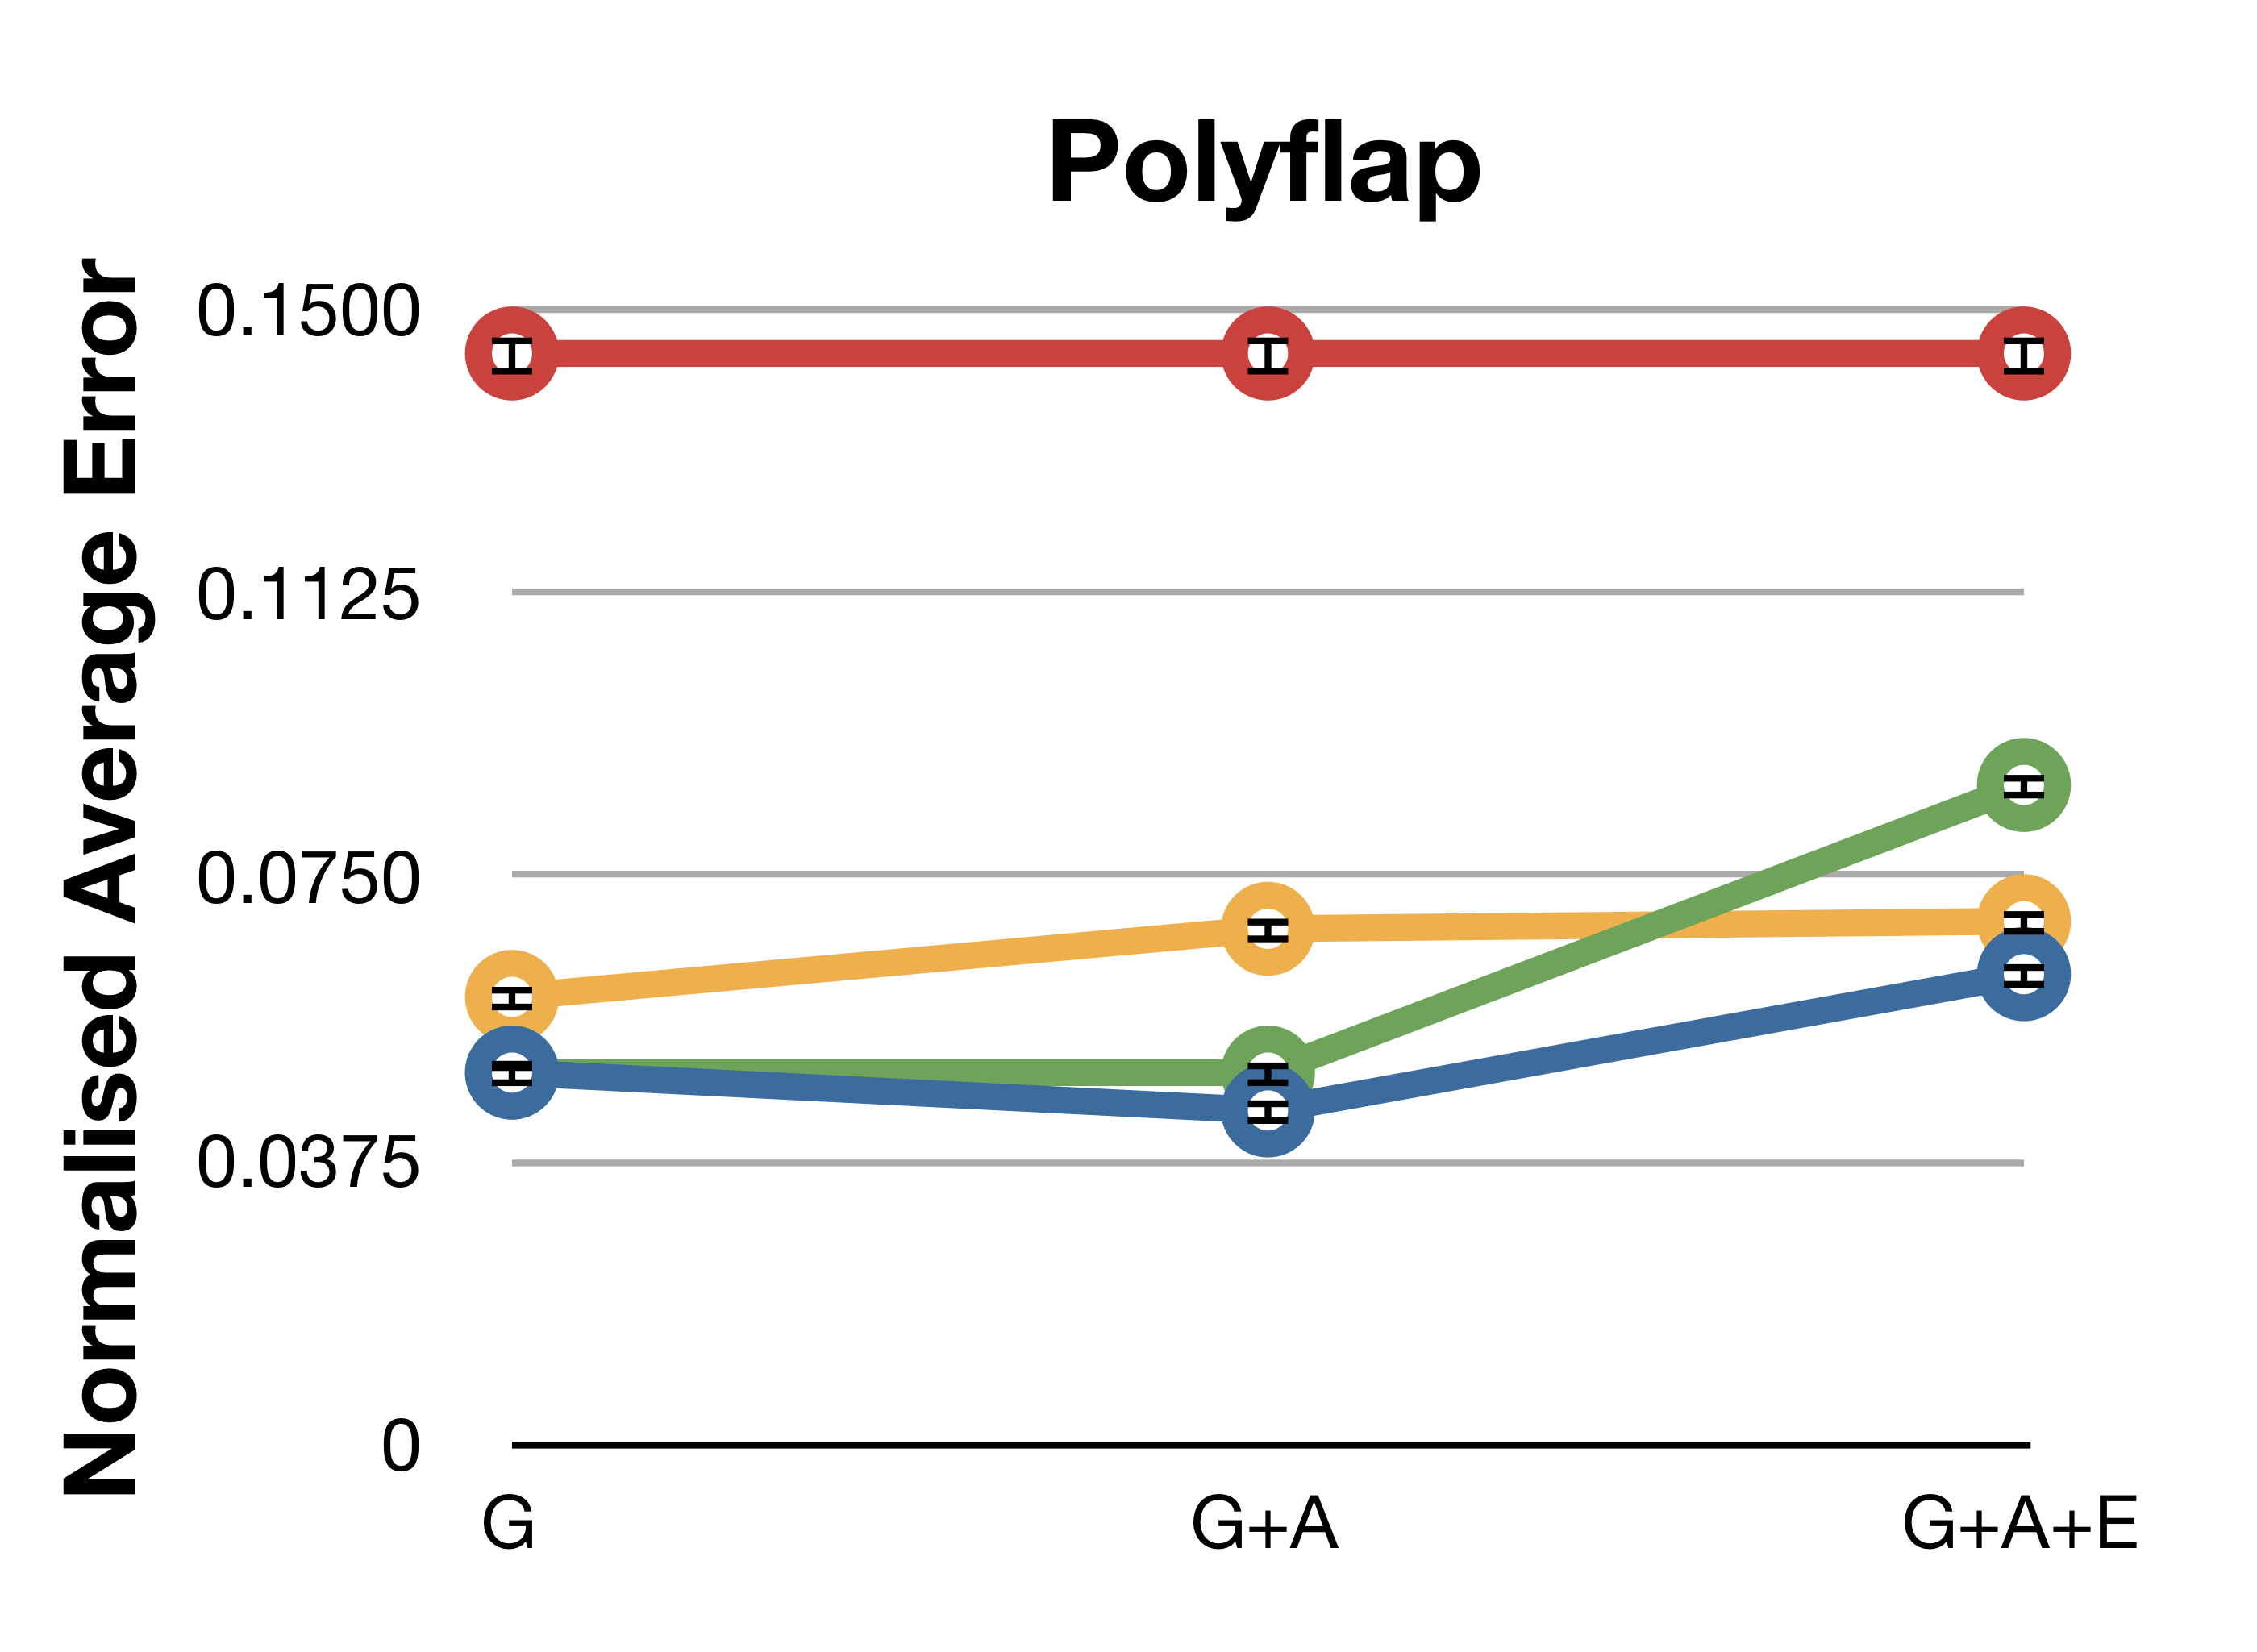
\includegraphics[width=0.45\columnwidth]{graphs_jw/L1av_graph_polyflap}
%}
%\centerline{
%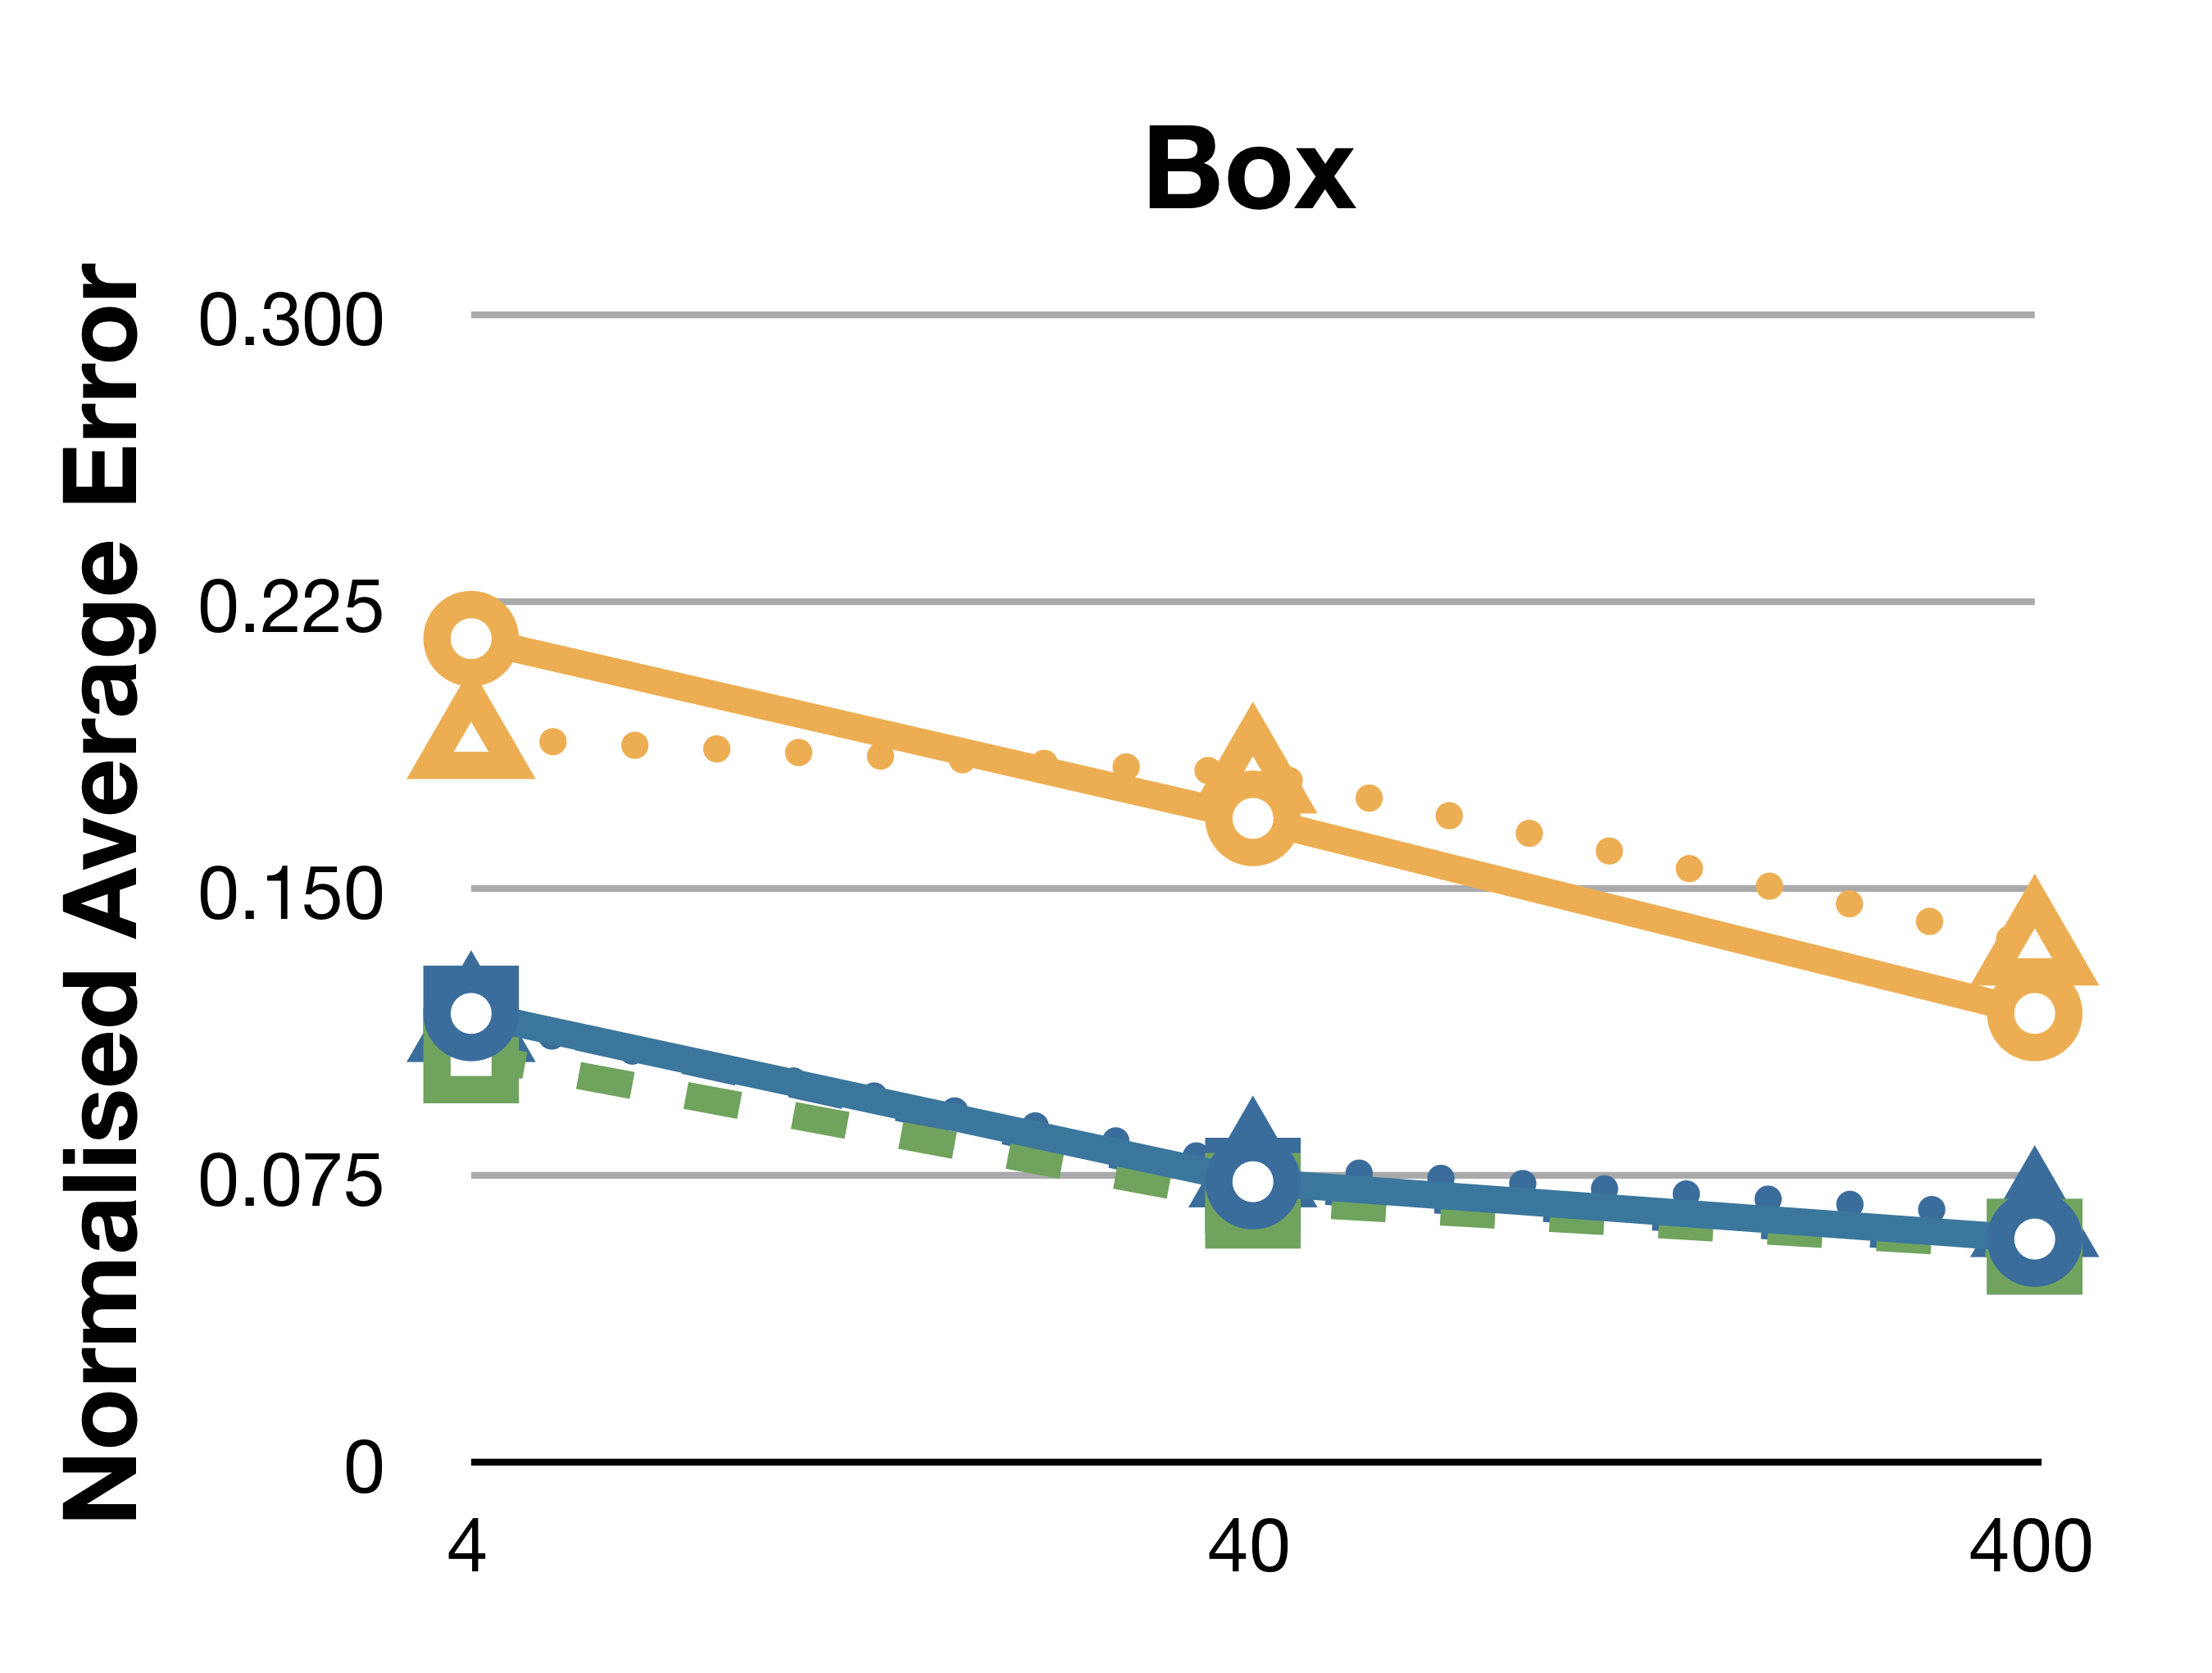
\includegraphics[width=0.45\columnwidth]{graphs_jw/L2av_graph}
%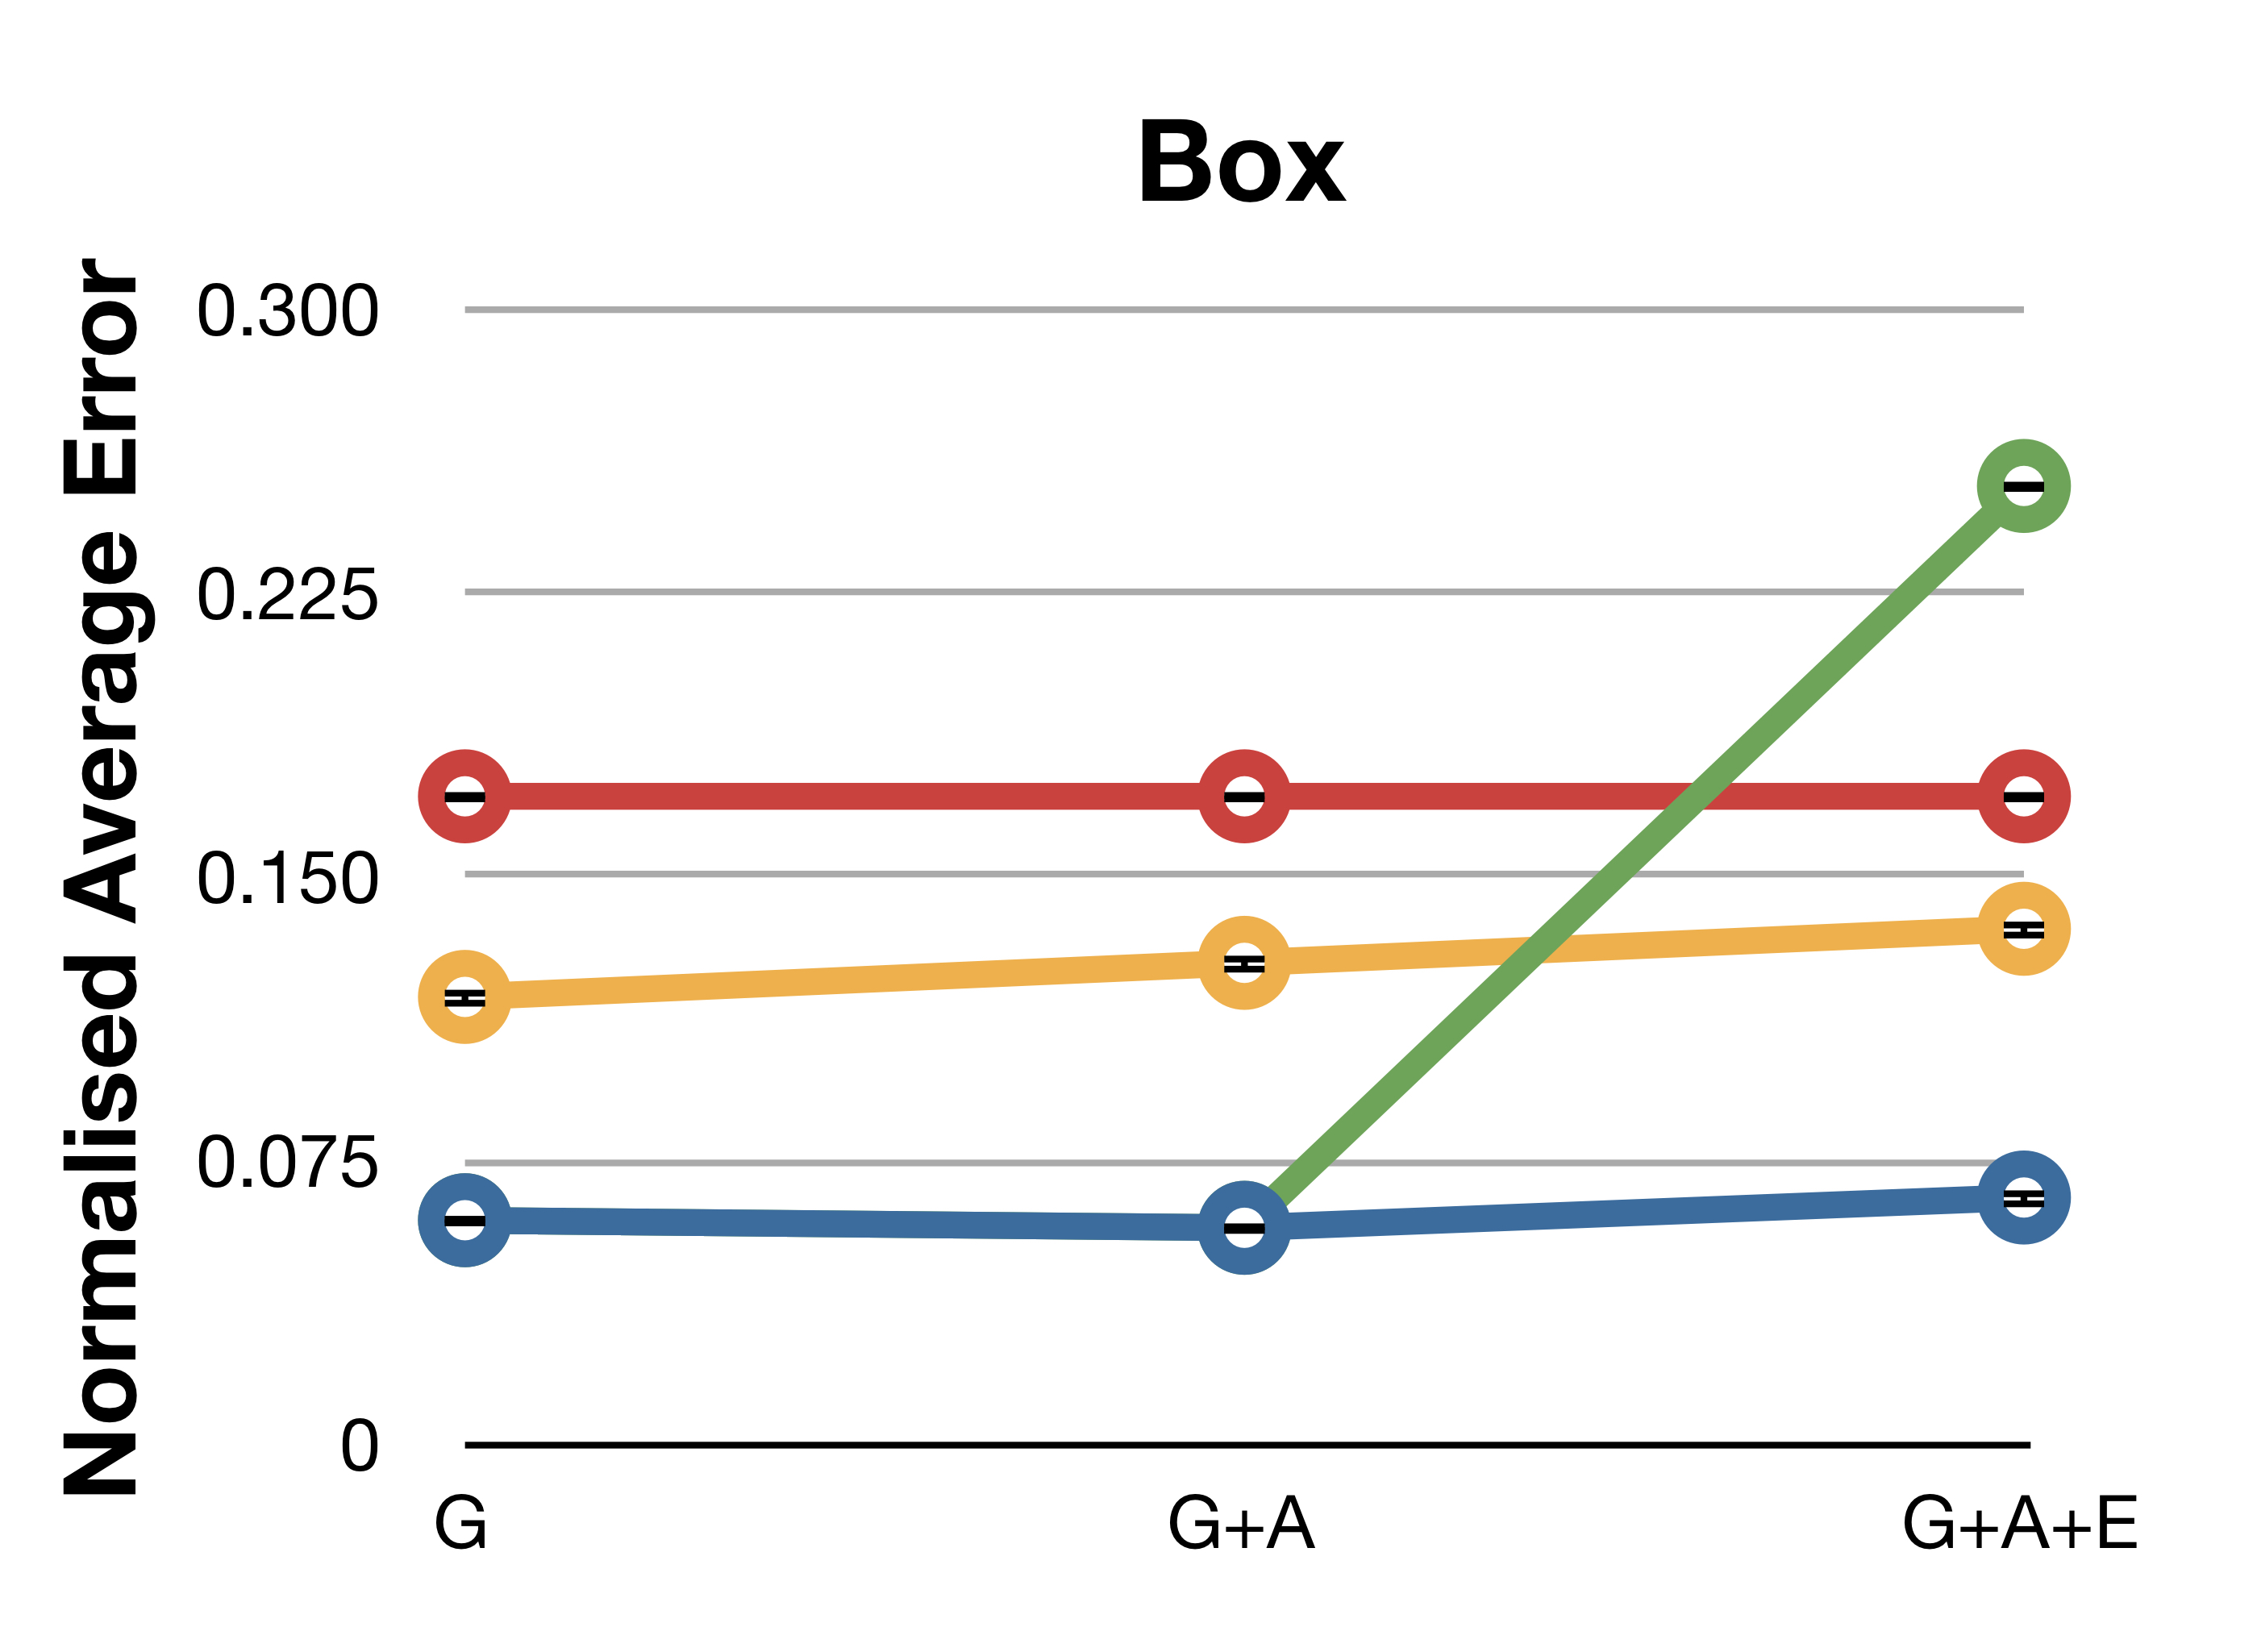
\includegraphics[width=0.45\columnwidth]{graphs_jw/L1av_graph_box}
%}
%\centerline{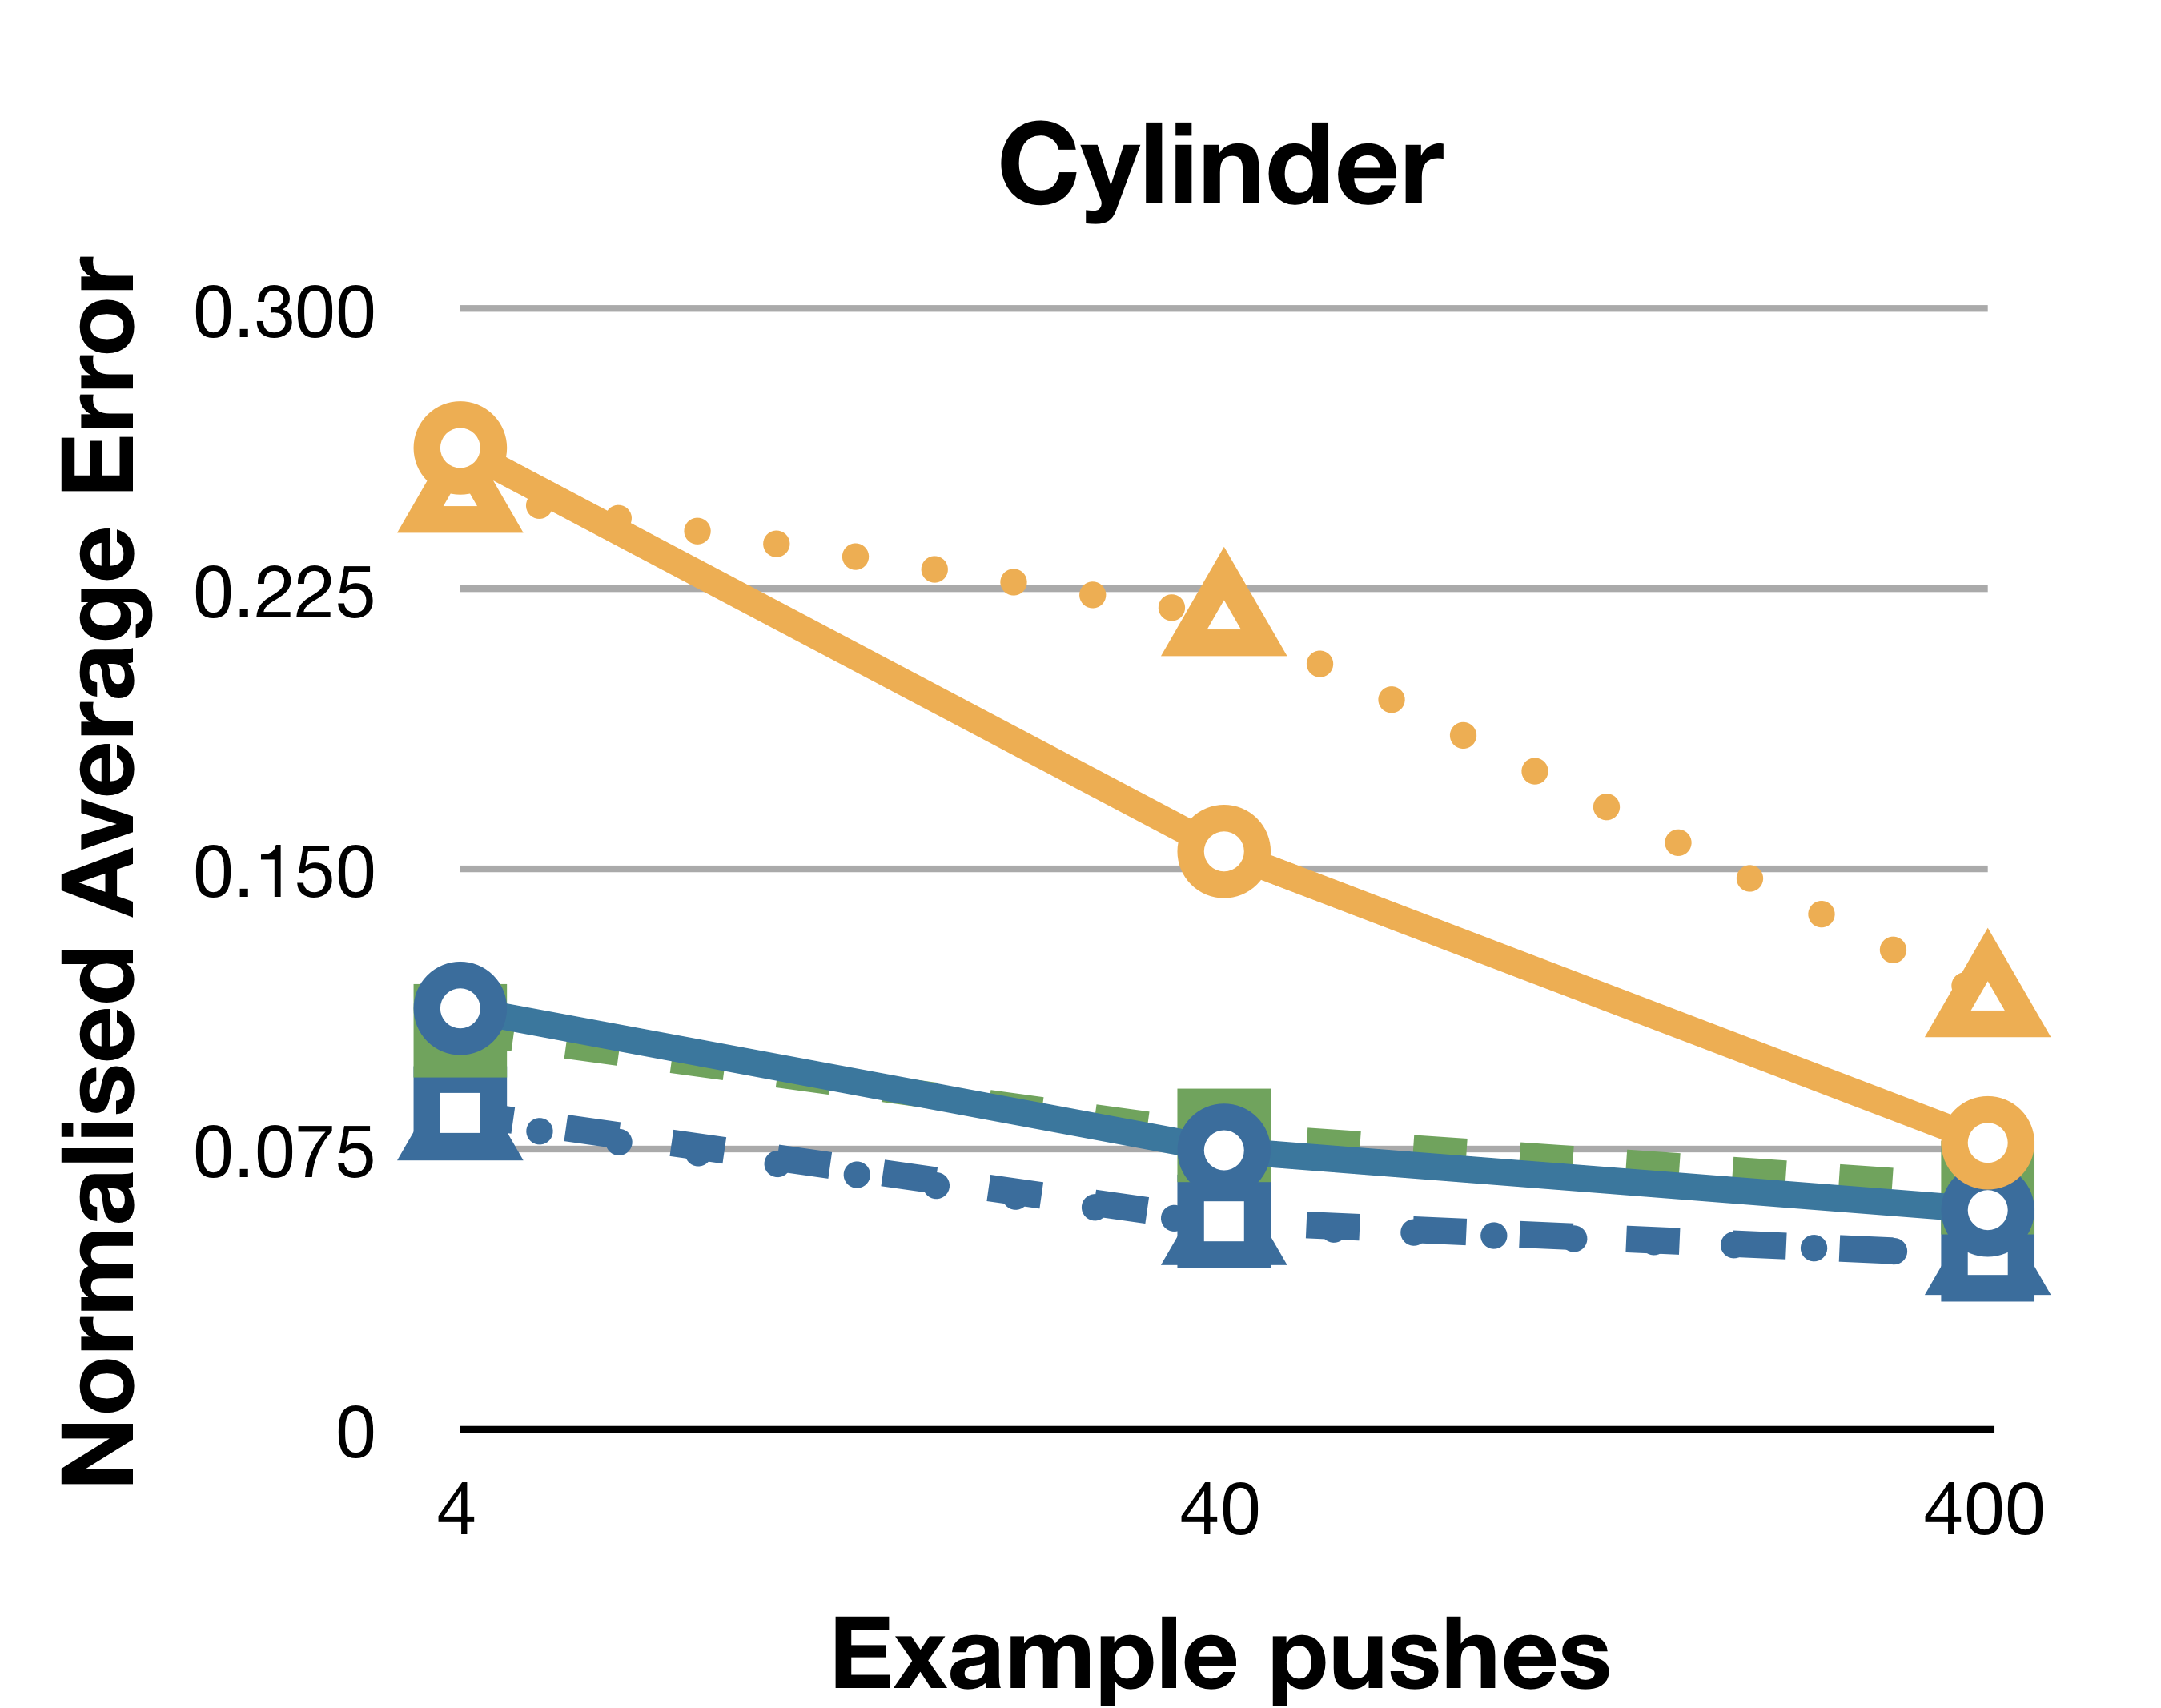
\includegraphics[width=0.45\columnwidth]{graphs_jw/L3av_graph}
%                 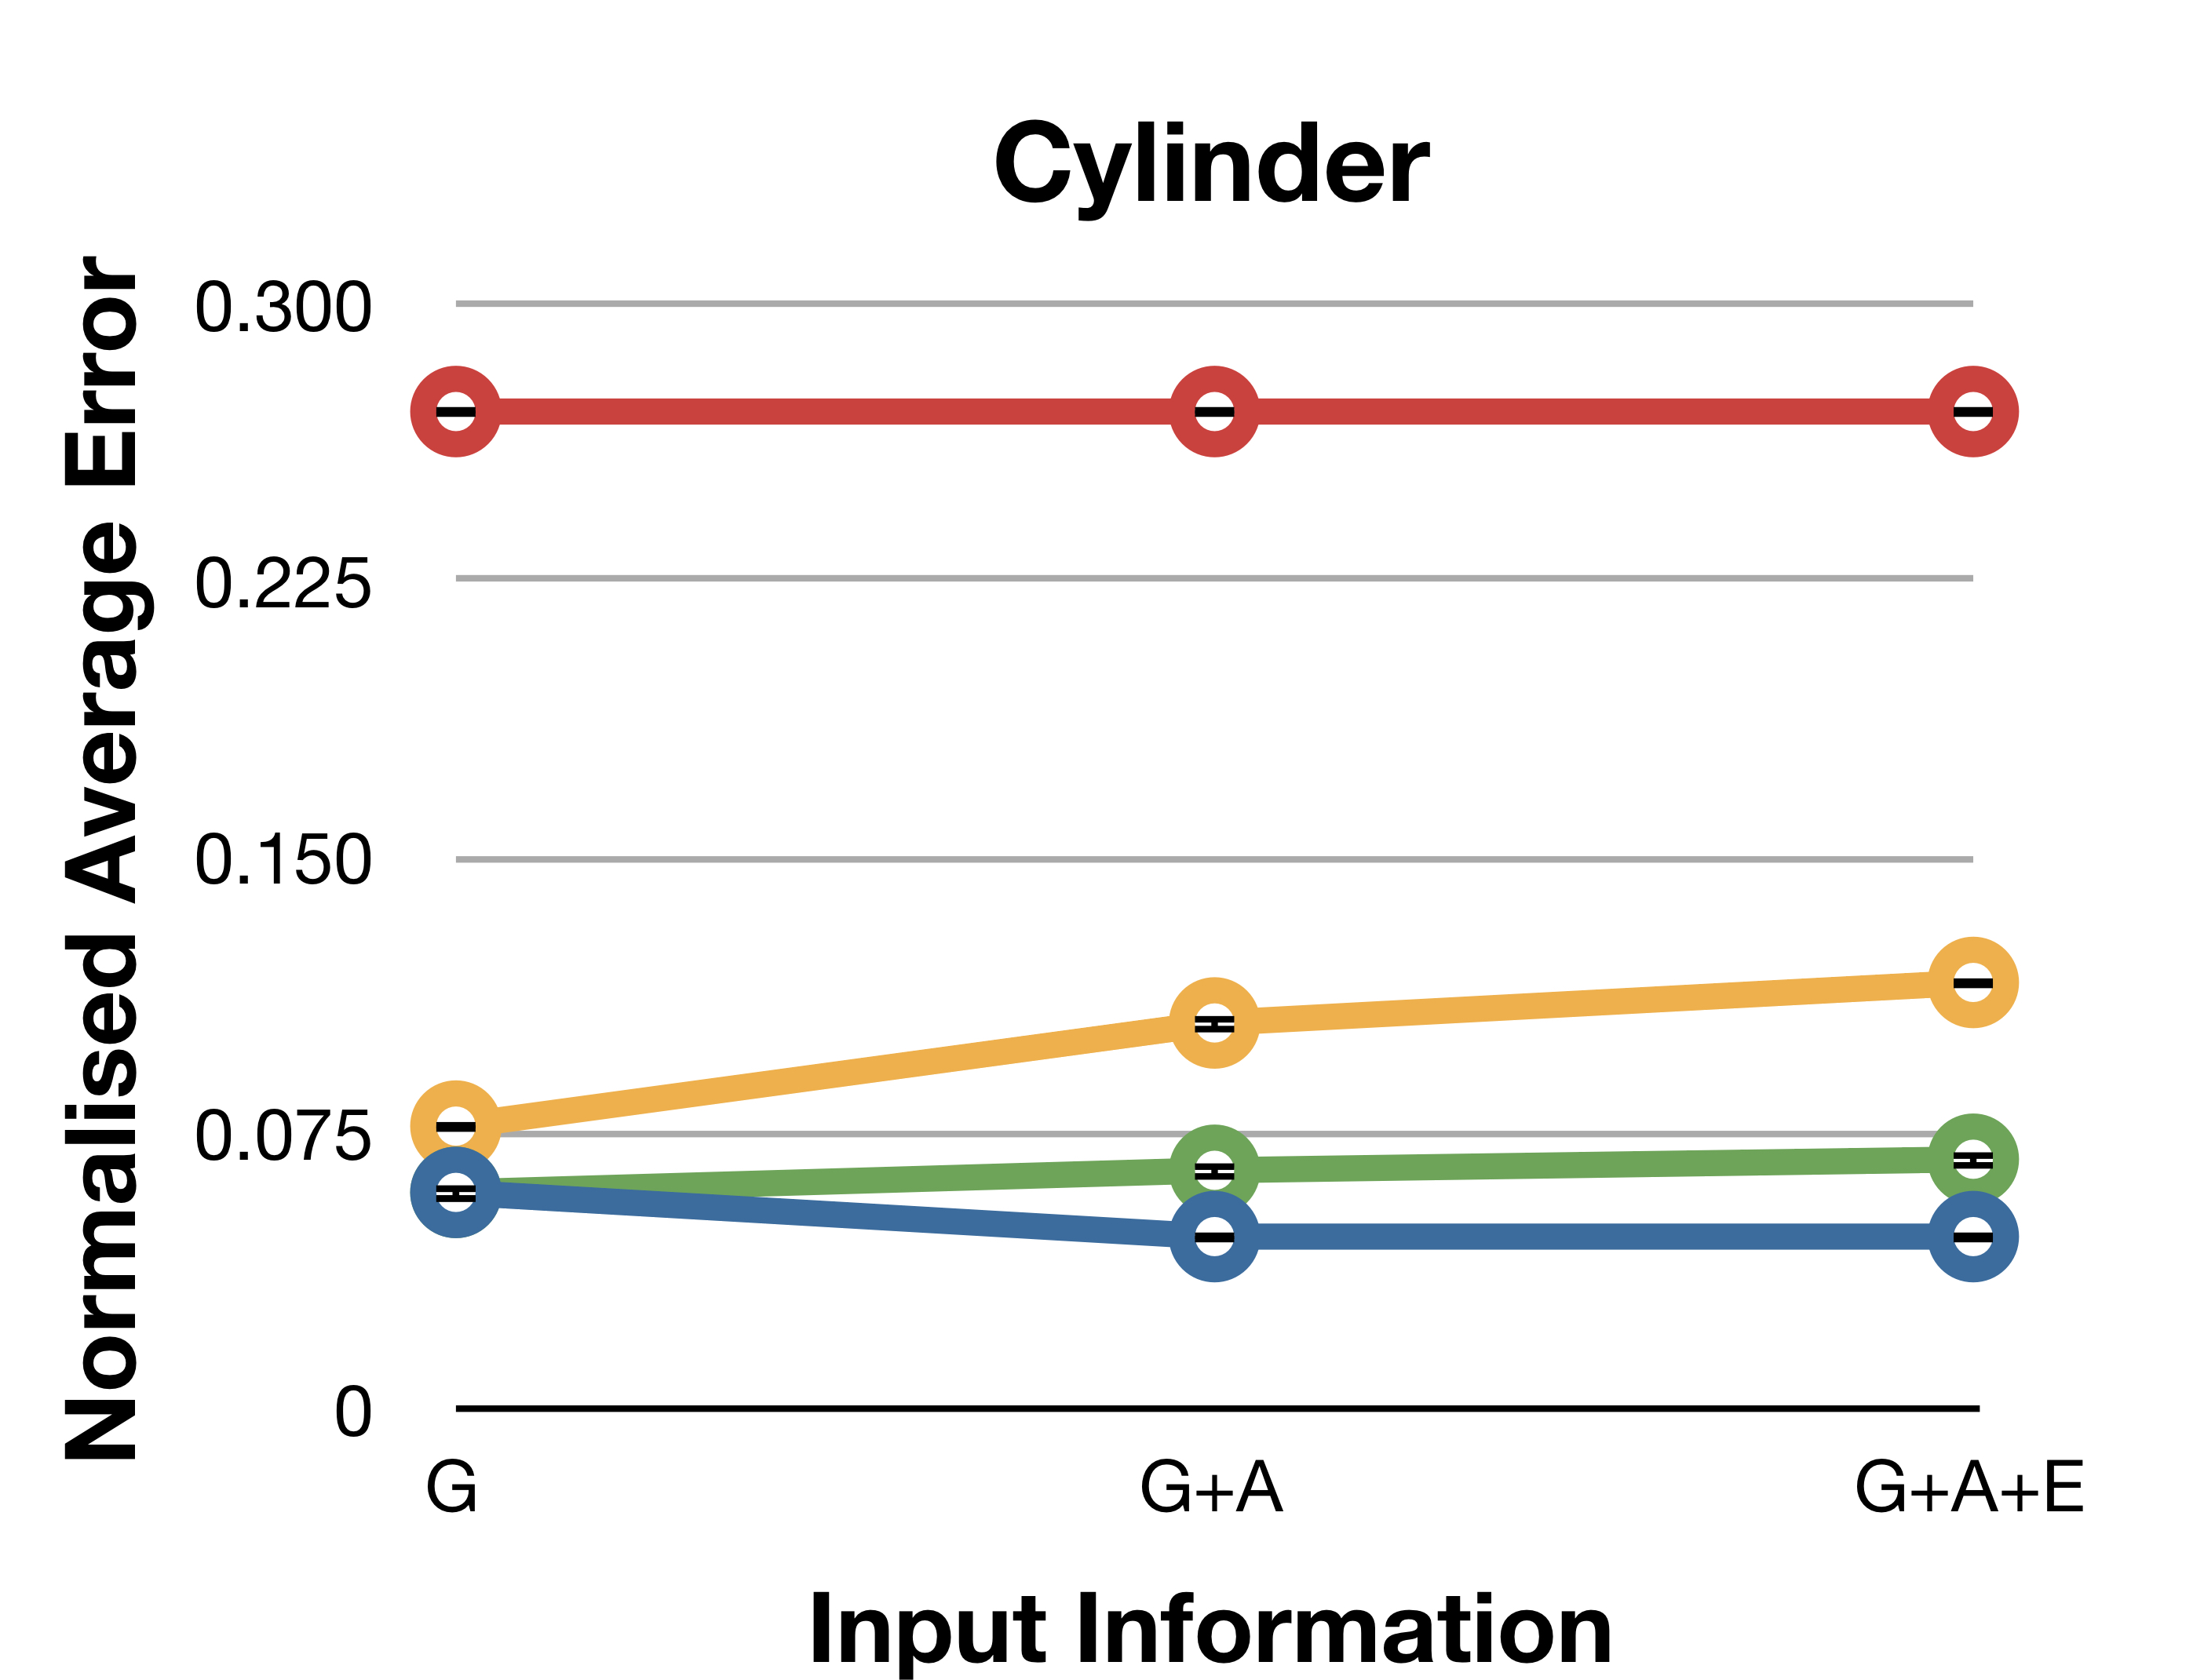
\includegraphics[width=0.45\columnwidth]{graphs_jw/L1av_graph_cylinder}
%}
%\centerline{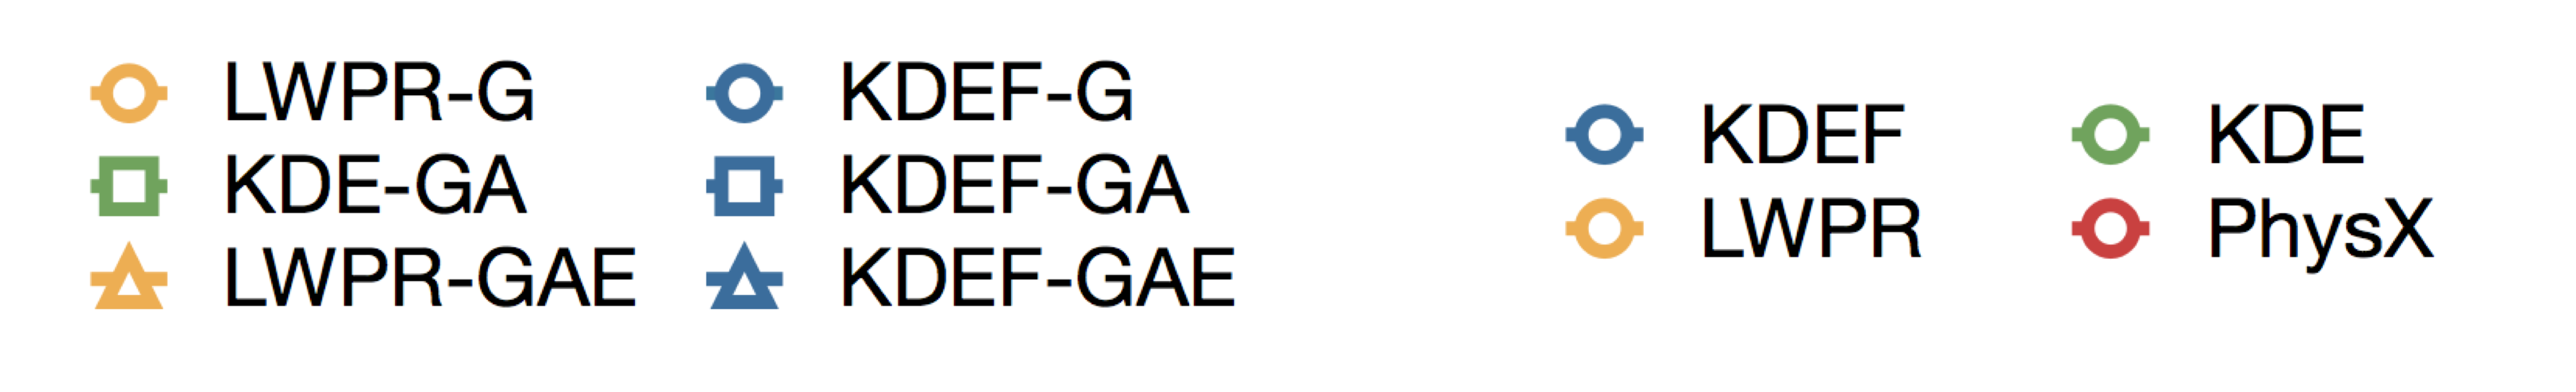
\includegraphics[width=\linewidth]{graphs_jw/L1_convergence_graph_key}
}
\vspace{-1mm}
\caption{Experiment P1: Convergence of a selection of learning
  algorithm-information combinations (left column). Change in normalised average prediction errors with varying input information (right column). G - global information; A - agent-object information; E - object-environment information.}
\label{fig:Lgraphs}
\end{figure}


\section{Results}\label{sec:Results}

\subsection{Experiment P1: Action Interpolation}\label{sec:Results.Learning}

In Experiment P1 the robot applied a set of random pushes to a
polyflap, a box and a cylinder respectively. All the algorithm
variants in Table~\ref{tab:algs} were trained and tested. Model
selection was performed for all algorithm-information combinations including PhysX. Ten fold cross-validation was performed for all algorithms. The density estimation techniques were studied with all three parameterisations of rotation. Training (and testing) sets were 200 (25) pushes (cylinder), 400 (50) pushes (box) and 700 (90) pushes (polyflap). Figure~\ref{fig:Lgraphs} (left column) shows convergence of the best learning algorithms. Figure~\ref{fig:Lgraphs} (right column) shows how performance varies with input information for the best parameterisations of all the algorithms. Table~\ref{tab:PerformanceTableL1av} shows the results of model selection on the different parameterisations for KDE. Image sequences of predicted vs actual trajectories are shown in (Figure~\ref{fig:ExperimentL2}).

\begin{table}[b]
\begin{center}
\begin{tabular}{|l|l|l|l|l|}
\cline{1-4}
Predictor & Polyflap & Box & Cylinder \\
\cline{1-4}
KDEF-G euler & 0.055$\pm$0.002 & 0.061$\pm$0.003 & 0.063$\pm$0.003\\
KDEF-G quat  & \textbf{0.049}$\pm$0.002 & \textbf{0.059}$\pm$0.002 & \textbf{0.059}$\pm$0.003\\
KDEF-G vmf   & 0.057$\pm$0.002 & 0.066$\pm$0.003 & 0.071$\pm$0.003\\
LWPR-G euler &  0.059$\pm$0.002 & 0.118$\pm$0.003 & 0.077$\pm$0.003\\
\cline{1-4}
KDEF-GA euler & 0.054$\pm$0.002 & 0.060$\pm$0.003 & 0.052$\pm$0.002\\
KDEF-GA quat & \textbf{0.044}$\pm$0.002 & \textbf{0.057}$\pm$0.002 & \textbf{0.047}$\pm$0.002\\
KDEF-GA vmf & 0.064$\pm$0.002 & 0.097$\pm$0.002  & 0.109$\pm$0.003 \\
LWPR-GA euler & 0.068$\pm$0.002 & 0.127$\pm$0.003 & 0.105$\pm$0.002 \\
\cline{1-4}
KDEF-GAE euler & 0.083$\pm$0.003 & 0.065$\pm$0.003 & 0.050$\pm$0.002 \\
KDEF-GAE quat & \textbf{0.062}$\pm$0.002 & \textbf{0.065}$\pm$0.003 & \textbf{0.047}$\pm$0.002\\
KDEF-GAE vmf & 0.081$\pm$0.002 & 0.086$\pm$0.002 & 0.065$\pm$0.002\\
LWPR-GAE euler & 0.069$\pm$0.002 & 0.136$\pm$0.003 & 0.116$\pm$0.003\\
\cline{1-4}
KDE-GA euler & 0.053$\pm$0.002 & 0.057$\pm$0.002 & 0.068$\pm$0.003 \\
KDE-GA quat  & \textbf{0.049}$\pm$0.002 & \textbf{0.057}$\pm$0.002 & \textbf{0.065}$\pm$0.003\\
KDE-GA vmf   & 0.062$\pm$0.002 & 0.058$\pm$0.002 & 0.092$\pm$0.004\\
\cline{1-4}
KDE-GAE euler & 0.090$\pm$0.002 & 0.161$\pm$0.003 & 0.071$\pm$0.003\\
KDE-GAE quat  & \textbf{0.087}$\pm$0.002 & 0.253$\pm$0.002 & \textbf{0.068}$\pm$0.003\\
KDE-GAE vmf   & \textbf{0.087}$\pm$0.002 & \textbf{0.127}$\pm$0.003 & 0.091$\pm$0.004\\
\cline{1-4}
PhysX & 0.144$\pm$0.003 &  0.171$\pm$0.003 & 0.271$\pm$0.001\\
\cline{1-4}
\end{tabular}
\end{center}
\caption[Performance Table]{Experiment P1: Forward push on a
  polyflap/box/cylinder, trained on real data. Shown is the dimensionless measure normalised average error  ${E_{av}^{norm}} \pm$ standard error.
}\label{tab:PerformanceTableL1av}
\end{table}

\newlength{\imgAXwid}
\setlength{\imgAXwid}{2.15cm}

{\bf Experiment P1 discussion.} Table~\ref{tab:PerformanceTableL1av} and Figure~\ref{fig:Lgraphs} show that the learned models almost always outperformed the physics simulator on the test set, with approximately one third the prediction error. Thus we find strong support for hypothesis H1. Regarding the parameterisation, Gaussian kernels with quaternions were best in 14 of 15 cases  (Table~\ref{tab:PerformanceTableL1av} boldentries). Thus in experiments P2 and P3 this parameterisation was used for the density estimation algorithms.

\begin{figure*}[htbp]
\centerline{
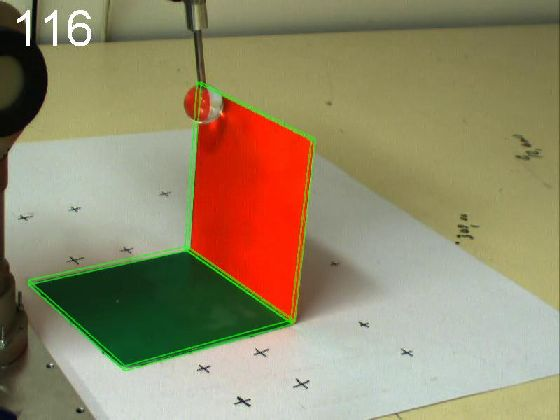
\includegraphics[width=\imgAXwid]{images/A1_2exp_667_1}
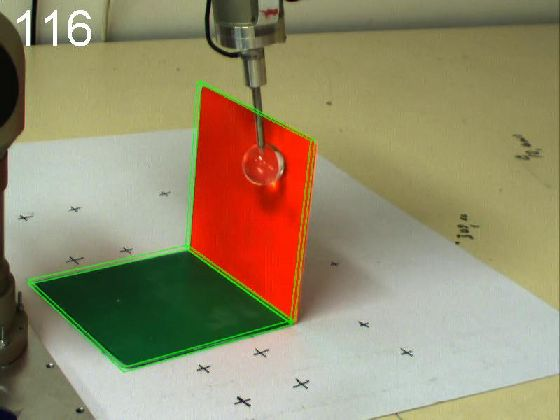
\includegraphics[width=\imgAXwid]{images/A1_2exp_876_1}
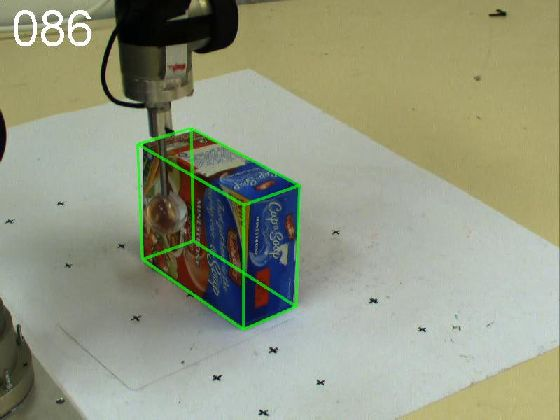
\includegraphics[width=\imgAXwid]{images/A2_2exp_399_1}
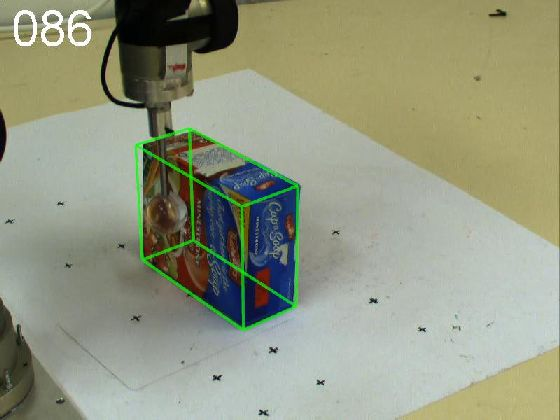
\includegraphics[width=\imgAXwid]{images/A2_LWPR1_399_1}
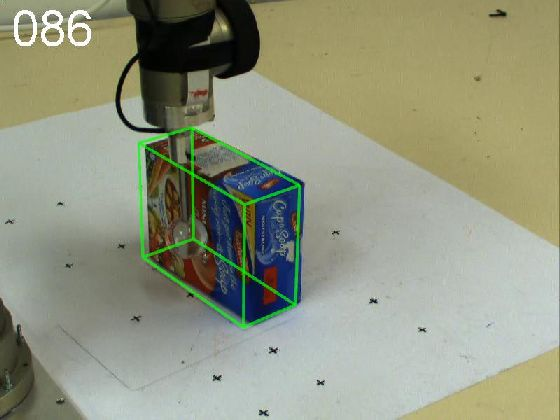
\includegraphics[width=\imgAXwid]{images/A2_2exp_87_1}
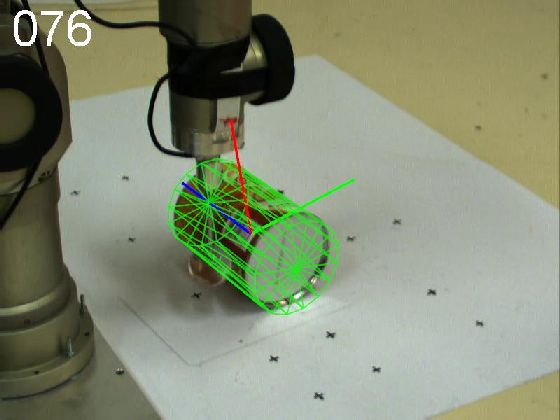
\includegraphics[width=\imgAXwid]{images/A3_2exp_39_1}
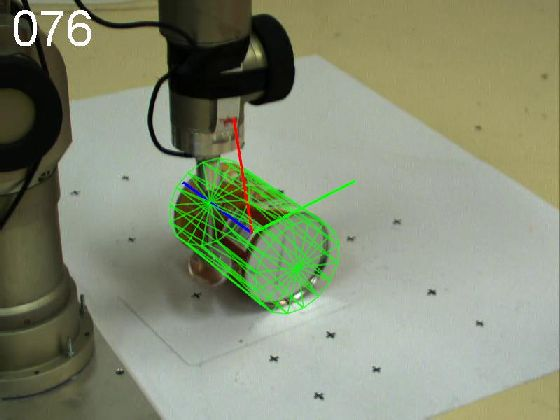
\includegraphics[width=\imgAXwid]{images/A3_LWPR1_39_1}
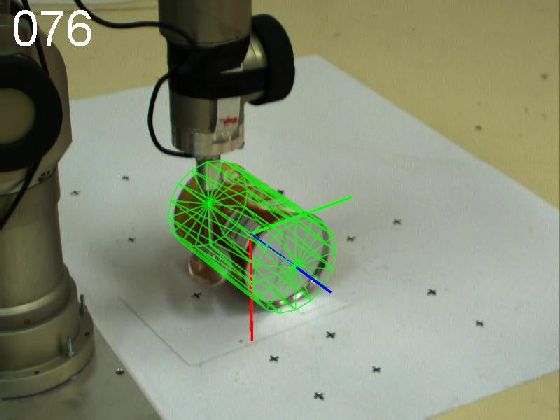
\includegraphics[width=\imgAXwid]{images/A3_physx_39_1}
}
\centerline{
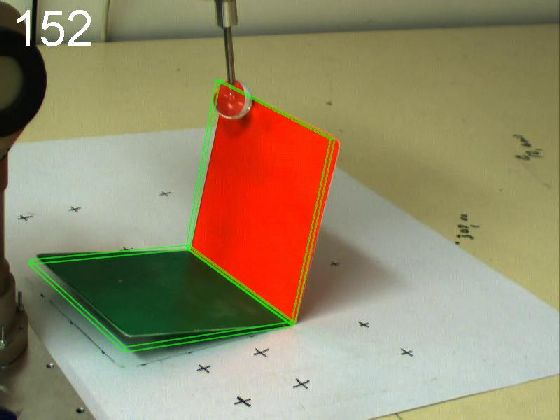
\includegraphics[width=\imgAXwid]{images/A1_2exp_667_2}
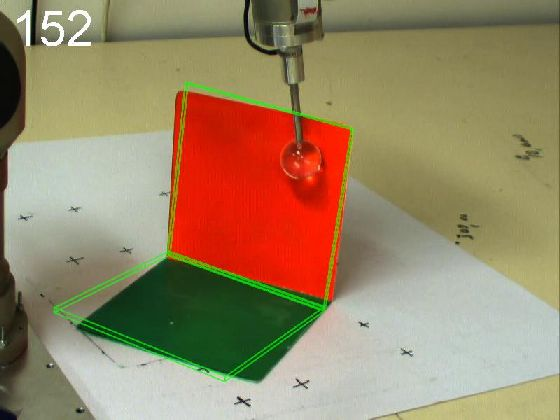
\includegraphics[width=\imgAXwid]{images/A1_2exp_876_2}
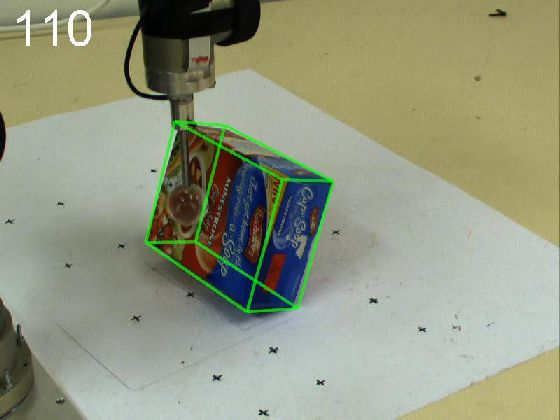
\includegraphics[width=\imgAXwid]{images/A2_2exp_399_2}
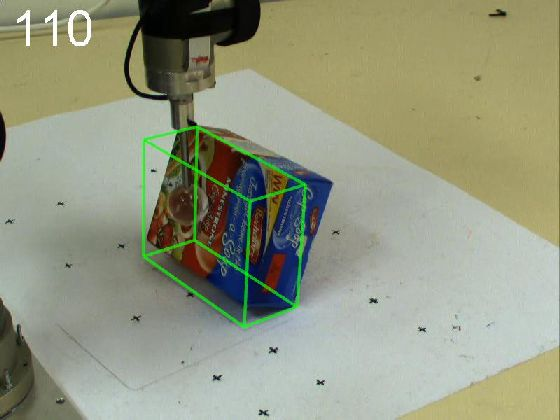
\includegraphics[width=\imgAXwid]{images/A2_LWPR1_399_2}
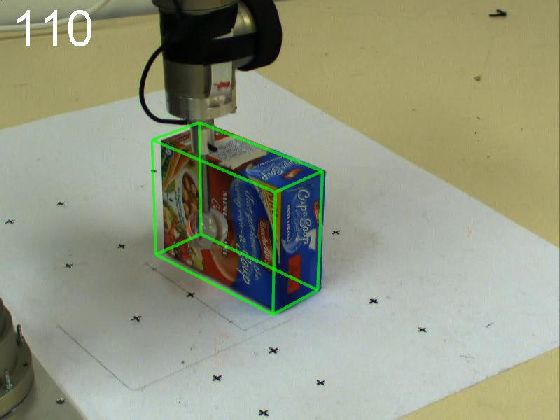
\includegraphics[width=\imgAXwid]{images/A2_2exp_87_2}
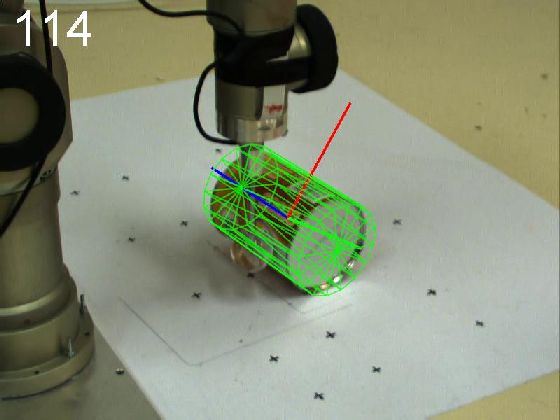
\includegraphics[width=\imgAXwid]{images/A3_2exp_39_2}
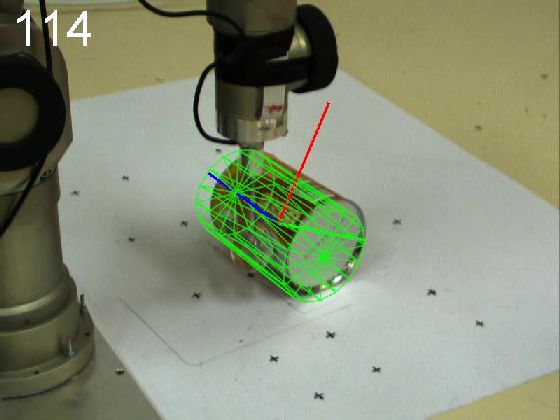
\includegraphics[width=\imgAXwid]{images/A3_LWPR1_39_2}
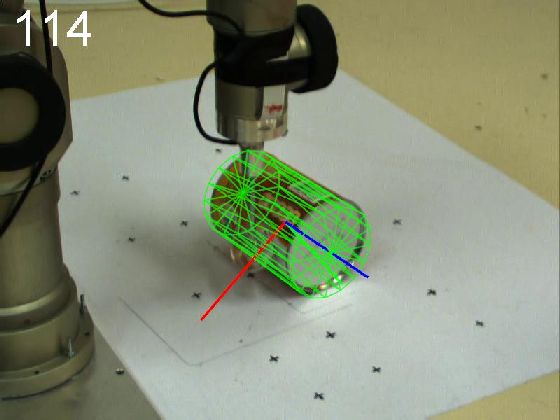
\includegraphics[width=\imgAXwid]{images/A3_physx_39_2}
}
% problem with physx @@@
%\vspace{0.1cm}
%\centerline{
%\includegraphics[width=\imgAXwid]{images/A2_physx_399_1}
%\includegraphics[width=\imgAXwid]{images/A2_physx_399_2}
%\includegraphics[width=\imgAXwid]{images/A2_physx_399_3}
%\includegraphics[width=\imgAXwid]{images/A2_physx_399_4}
%\includegraphics[width=\imgAXwid]{images/A2_physx_399_5}
%}
%\vspace{0.1cm}
\centerline{
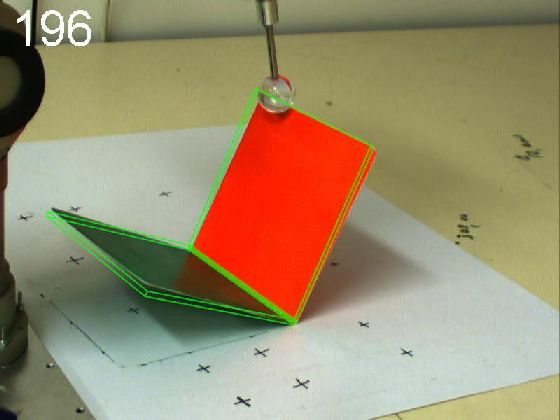
\includegraphics[width=\imgAXwid]{images/A1_2exp_667_3}
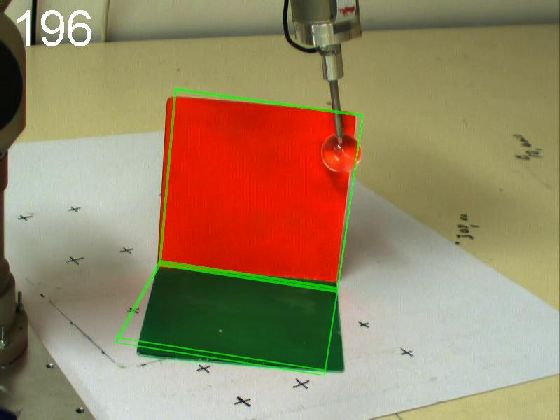
\includegraphics[width=\imgAXwid]{images/A1_2exp_876_3}
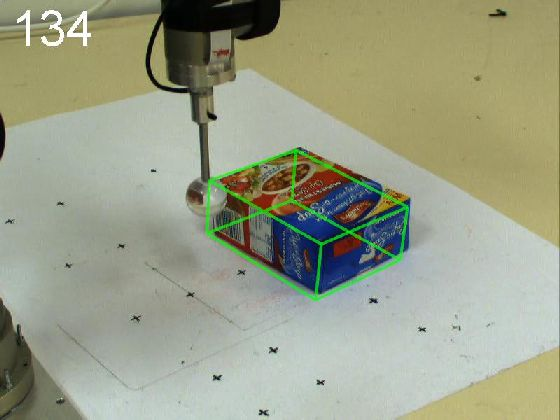
\includegraphics[width=\imgAXwid]{images/A2_2exp_399_3}
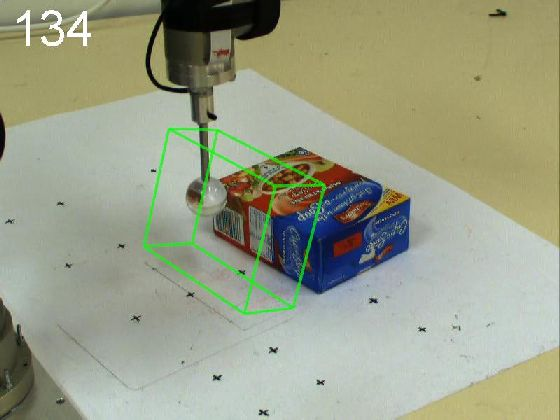
\includegraphics[width=\imgAXwid]{images/A2_LWPR1_399_3}
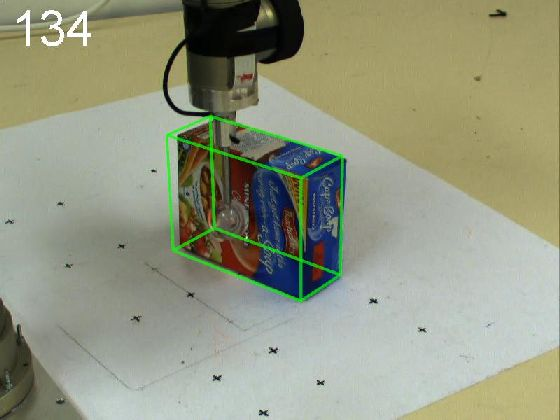
\includegraphics[width=\imgAXwid]{images/A2_2exp_87_3}
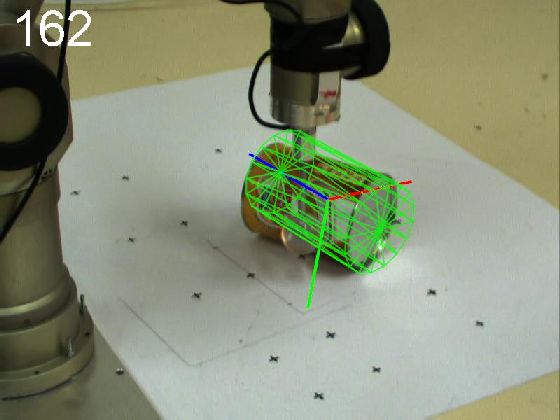
\includegraphics[width=\imgAXwid]{images/A3_2exp_39_3}
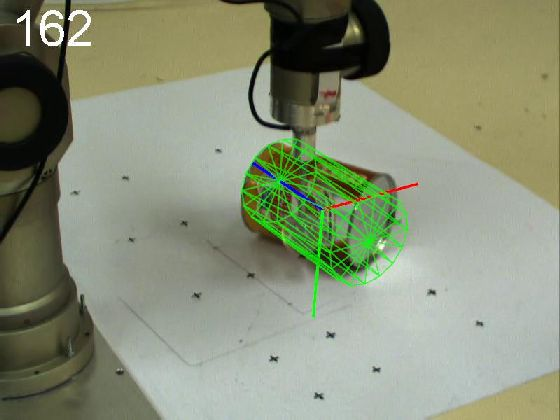
\includegraphics[width=\imgAXwid]{images/A3_LWPR1_39_3}
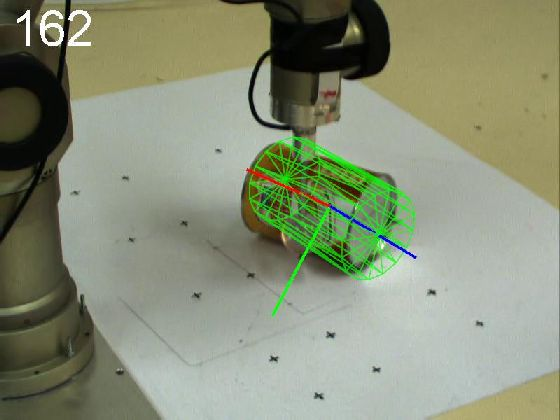
\includegraphics[width=\imgAXwid]{images/A3_physx_39_3}
}
\centerline{
\includegraphics[width=\imgAXwid]{images/A1_2exp_667_4}
\includegraphics[width=\imgAXwid]{images/A1_2exp_876_4}
\includegraphics[width=\imgAXwid]{images/A2_2exp_399_4}
\includegraphics[width=\imgAXwid]{images/A2_LWPR1_399_4}
\includegraphics[width=\imgAXwid]{images/A2_2exp_87_4}
\includegraphics[width=\imgAXwid]{images/A3_2exp_39_4}
\includegraphics[width=\imgAXwid]{images/A3_LWPR1_39_4}
\includegraphics[width=\imgAXwid]{images/A3_physx_39_4}
}
%\vspace{0.1cm}
\centerline{
\includegraphics[width=\imgAXwid]{images/A1_2exp_667_5}
\includegraphics[width=\imgAXwid]{images/A1_2exp_876_5}
\includegraphics[width=\imgAXwid]{images/A2_2exp_399_5}
\includegraphics[width=\imgAXwid]{images/A2_LWPR1_399_5}
\includegraphics[width=\imgAXwid]{images/A2_2exp_87_5}
\includegraphics[width=\imgAXwid]{images/A3_2exp_39_5}
\includegraphics[width=\imgAXwid]{images/A3_LWPR1_39_5}
\includegraphics[width=\imgAXwid]{images/A3_physx_39_5}
}
%\vspace{0.1cm}
\caption {Experiment P1: polyflap, box and cylinder. Green outline shows
  predictions. Columns 1-2: KDEF-GA/quat on two trials exhibiting
  different motions of the polyflap. Col 3: KDEF-GA/quat. Col 4: LWPR-G for one trial in
  which the box topples over. Col 5: KDEF-GA/quat on another trial in
  which the box slides. Columns 6-8 show the same push of the
  cylinder. Col 6: KDEF-GA/quat. Col 7: LWPR-G. Col 8: PhysX. Note tha
  for columns 6-7 the orientation of the cylinder is show by the
  rotating frame. Only the learned models predict the rotation
  correctly.(The
  frame number is shown in the top left of each image.)  }
\label{fig:ExperimentL2}
\end{figure*}

In Figure~\ref{fig:ExperimentL2} it can be
seen that predictions were accurate and physically plausible for a
variety of learning methods even over 150 steps. Note the physics
simulator predicts incorrect turning of the cylinder when pushed
(Figure~\ref{fig:ExperimentL2} column 8). Finally Figure~\ref{fig:Lgraphs} shows that additional information A or E gives no advantage for any algorithm in this experiment, indeed LWPR gets worse with more dimensions. This is in line with expectation, since no learning transfer is being attempted.

\subsection{Experiment P2: Action Transfer}
\label{sec:Results.Action}

\begin{figure}[t]
%\centerline{\includegraphics[width=0.9\columnwidth]{graphs_jw/A_real_sim_av_graph}}
%\centerline{\includegraphics[width=0.45\columnwidth]{graphs_jw/A_sim_av_graph.png}%}
%\centerline{
%\includegraphics[width=0.46\columnwidth]{graphs_jw/A_real_av_graph.png}}
\centerline{\includegraphics[width=\columnwidth]{graphs_jw/P2-graphs}}
\caption{Experiment P2: Action transfer. Trained on forward push on polyflap, tested on backward push, for simulated (top) and real data (bottom). Comparative performance of predictors vs. information utilised (global/agent/environment),
as measured by normalised average error ${E_{av}^{norm}}$.
%Also included is a single data point for the PhysX physics engine.
}\label{fig:A_av_graphs}
\end{figure}

Experiment P2 tests hypothesis H2: whether predictions can be
transfered to novel actions.  The training set was 900 pushes applied to an L shaped flap in one direction (Figure~\ref{fig:ToyExample} top
left).  The test set was 100 pushes applied from the other side (Figure~\ref{fig:ToyExample} top right). The same method was followed in simulation and with the real object. All the algorithm-information variants in Table~\ref{tab:algs} were tested. We measured the transfer prediction error, i.e.\ the prediction error for the novel test actions. Figure~\ref{fig:A_av_graphs} %(also see Table~\ref{tab:PerformanceTableAav})
shows the normalised average error $E_{av}^{norm}$ for the simulation experiment (left panel) and with real objects (right panel).
Figure~\ref{fig:ExperimentA} shows example predicted trajectories on
synthetic and real test cases.

% @@@ COMMENT ON KDE-GAX RESULTS
% \begin{figure*}[tbp]
% \centerline{
% \includegraphics[width=2.3cm]{images/B1_1exp_20_1}
% \includegraphics[width=2.3cm]{images/B1_1exp_20_2}
% \includegraphics[width=2.3cm]{images/B1_1exp_20_3}
% \includegraphics[width=2.3cm]{images/B1_1exp_20_4}
% \includegraphics[width=2.3cm]{images/B1_1exp_20_5}
% }
% \vspace{0.1cm}
% \centerline{
% \includegraphics[width=2.3cm]{images/B1_2exp_20_1}
% \includegraphics[width=2.3cm]{images/B1_2exp_20_2}
% \includegraphics[width=2.3cm]{images/B1_2exp_20_3}
% \includegraphics[width=2.3cm]{images/B1_2exp_20_4}
% \includegraphics[width=2.3cm]{images/B1_2exp_20_5}
% }
% \vspace{0.1cm}
% \centerline{
% \includegraphics[width=2.3cm]{images/B1_3exp_20_1}
% \includegraphics[width=2.3cm]{images/B1_3exp_20_2}
% \includegraphics[width=2.3cm]{images/B1_3exp_20_3}
% \includegraphics[width=2.3cm]{images/B1_3exp_20_4}
% \includegraphics[width=2.3cm]{images/B1_3exp_20_5}
% }
% %\vspace{0.1cm}
% %\centerline{
% %\includegraphics[width=2.3cm]{images/B1_3exp_61_1}
% %\includegraphics[width=2.3cm]{images/B1_3exp_61_2}
% %\includegraphics[width=2.3cm]{images/B1_3exp_61_3}
% %\includegraphics[width=2.3cm]{images/B1_3exp_61_4}
% %\includegraphics[width=2.3cm]{images/B1_3exp_61_5}
% %}
% \caption
% {Experiment A (simulation):
% Green outline shows predictions (from top row to bottom row) by

% compared to simulated `ground truth' (in cyan).
% These predictions illustrate the rationale for extra contact information
% presented in Figure~\ref{fig:ToyExample}.
% (The frame number is shown in the top left of each image.)
% }
% \label{fig:ExperimentA}
% \end{figure*}

\newlength{\imgBXwid}
\setlength{\imgBXwid}{2.15cm}
\begin{figure*}[tb]
\centerline{
\includegraphics[width=\imgBXwid]{images/B1_1exp_20_1}
\includegraphics[width=\imgBXwid]{images/B1_2exp_20_1}
\includegraphics[width=\imgBXwid]{images/B1_3exp_20_1}
\includegraphics[width=\imgBXwid]{images/B2_2exp_58_1}
\includegraphics[width=\imgBXwid]{images/B2_1exp_58_1}
\includegraphics[width=\imgBXwid]{images/B2_LWPR1_58_1}
\includegraphics[width=\imgBXwid]{images/B2_2exp_38_1}
}
%\vspace{0.1cm}
\centerline{
\includegraphics[width=\imgBXwid]{images/B1_1exp_20_2}
\includegraphics[width=\imgBXwid]{images/B1_2exp_20_2}
\includegraphics[width=\imgBXwid]{images/B1_3exp_20_2}
\includegraphics[width=\imgBXwid]{images/B2_2exp_58_2}
\includegraphics[width=\imgBXwid]{images/B2_1exp_58_2}
\includegraphics[width=\imgBXwid]{images/B2_LWPR1_58_2}
\includegraphics[width=\imgBXwid]{images/B2_2exp_38_2}
}
%\vspace{0.1cm}
\centerline{
\includegraphics[width=\imgBXwid]{images/B1_1exp_20_3}
\includegraphics[width=\imgBXwid]{images/B1_2exp_20_3}
\includegraphics[width=\imgBXwid]{images/B1_3exp_20_3}
\includegraphics[width=\imgBXwid]{images/B2_2exp_58_3}
\includegraphics[width=\imgBXwid]{images/B2_1exp_58_3}
\includegraphics[width=\imgBXwid]{images/B2_LWPR1_58_3}
\includegraphics[width=\imgBXwid]{images/B2_2exp_38_3}
}

\centerline{
\includegraphics[width=\imgBXwid]{images/B1_1exp_20_4}
\includegraphics[width=\imgBXwid]{images/B1_2exp_20_4}
\includegraphics[width=\imgBXwid]{images/B1_3exp_20_4}
\includegraphics[width=\imgBXwid]{images/B2_2exp_58_4}
\includegraphics[width=\imgBXwid]{images/B2_1exp_58_4}
\includegraphics[width=\imgBXwid]{images/B2_LWPR1_58_4}
\includegraphics[width=\imgBXwid]{images/B2_2exp_38_4}
}
%\vspace{0.1cm}
\centerline{
\includegraphics[width=\imgBXwid]{images/B1_1exp_20_5}
\includegraphics[width=\imgBXwid]{images/B1_2exp_20_5}
\includegraphics[width=\imgBXwid]{images/B1_3exp_20_5}
\includegraphics[width=\imgBXwid]{images/B2_2exp_58_5}
\includegraphics[width=\imgBXwid]{images/B2_1exp_58_5}
\includegraphics[width=\imgBXwid]{images/B2_LWPR1_58_5}
\includegraphics[width=\imgBXwid]{images/B2_2exp_38_5}
}
\caption
{Experiment P2: Green outline shows predictions. Column 1: KDEF-G/quat. Col 2:
KDEF-GA/quat. Col 3: KDEF-GAE/quat. Col 4: KDEF-GA/quat. Col 5:
KDEF-G/quat. Col 6: LWPR-G. Col 7: KDEF-GA/quat.
Note that the KDEF-G/quat and LWPR-G methods predict
that the robot finger passes through the polyflap.
(The frame number is shown in the top left of each image.)
}
\label{fig:ExperimentA}
\end{figure*}

{\bf Experiment P2 discussion:} Figure~\ref{fig:A_av_graphs} (left panel) shows that in simulation that additional contact information (A or AE) didn't improve performance of KDE and LWPR. In contrast factorisation could take advantage of the additional information: the performance of KDEF improved significantly. The predictions of KDEF (Figure~\ref{fig:ExperimentA}) precisely match the hypothesised
effects of adding contact information depicted in Figure~\ref{fig:ToyExample} (bottom row). With only global information the finger was predicted by KDEF to pass through the object (Figure~\ref{fig:ExperimentA} column 1). By adding the agent-object information the prediction of KDEF was that the object would move with the finger, but that it penetrated the table (Figure~\ref{fig:ExperimentA} column 2). By also adding object-environment information KDEF predicts that the object will slide along the table in contact with the finger (Figure~\ref{fig:ExperimentA} column 3). On real objects (Figure~\ref{fig:A_av_graphs} right panel) the learned predictors slightly outperform the physics engine, and accuracy of the predictions goes down. But additional contact information with factoring still enables KDEF to make physically plausible predictions. Figure~\ref{fig:ExperimentA} (columns 5 and 6) shows that KDEF-G and LWPR-G predict that the finger passes through the object, and that the object doesn't move. In Figure~\ref{fig:ExperimentA} (columns 4 and 7) KDEF-GA correctly predicts the sliding motion of the object. Only factoring enables this, the unfactored methods don't produce plausible predictions. This supports hypothesis H2: factoring enables action transfer. Transfer is best if the training observations are accurate, diminishing with training noise. 

\subsection{Experiment P3:  Shape Transfer}\label{sec:Results.Shape}

Experiment P3 tests hypothesis H3: can predictors learned from one or two objects transfer their predictions to an object of novel shape? The experiment was run in simulation and with real objects. Shape transfer was tested from i) a polyflap to a box (P3.A) and ii) a box and a cylinder to a double cylinder (P3.B). There were 900 training pushes on the polyflap and 200 test pushes on the box for i), and 200 training pushes (100 box, 100 cylinder) and 100 test pushes (double cylinder) for ii). This experiment ran on real objects for i) and ii) and in simulation for i), giving three train-test conditions in total. We have previously published results from simulation for i) \cite{kopicki-etal-icra11}. All algorithm-information combinations from Table~\ref{tab:algs} were tried. When learning from two objects the same number of factors (experts) were used for each object, and they were matched across the two objects by hand. This means each expert received a mix of data from each object, learning to encode both rolling and sliding or tipping motions.  The normalised average error for all three conditions $E_{av}^{norm}$ is shown in Figure~\ref{fig:S_av_graphs}. Example frames from the experiments are shown in Figure~\ref{fig:ExperimentStransfer}.

{\bf Experiment P3 discussion.} Shape transfer only occurs with additional contact information and with factoring, such as for the
KDEF-GA method in experiment P3.A (Figure~\ref{fig:ExperimentStransfer} column 1).  Learners with global information only predict that the finger passed  through the box (Figure~\ref{fig:ExperimentStransfer} columns 2 and 3). In experiment P3.A, of the learners, only factoring plus all the contact information (KDEF-GAE) produced physically plausible predictions. In Figure~\ref{fig:ExperimentStransfer} (column 6) KDEF-GAE predicts that the double-cylinder slides along the table, whereas KDEF-G and KDEF-GA predict it will penetrate the table (Figure~\ref{fig:ExperimentStransfer} columns 4 and 5). KDEF-GAE also makes physically plausible predictions for a novel real object 
(Figure~\ref{fig:ExperimentStransfer} column 7). None of the other learners could achieve this shape transfer learning. Only by using factoring plus all contact information was shape transfer learning achieved. In fact KDEF-GAE also matched the accuracy of the physics simulator. Thus this experiment supports hypothesis H3: factoring + contact information enables shape transfer learning.

\subsection{General Discussion:} There are two questions that arise from the experiments collectively. First why does PhysX fail to do better P1 even though separately tuned to each object? The answer is that real objects don't adhere to idealised friction models with one coefficient for each surface: flaws in object surfaces cause deviations from the tuned model. Thus the problem holds for all such simulators and so a modular learning model will always be better. Second, why does transfer learning decline on real data in P2 and P3? The answer is tracking noise in the training data, leading to perceived penetrations of the object by the finger, giving some probability in the model that the finger can pass through the object. 
%***ADD IMAGES TO ILLUSTRATE HOW LWPR ALWAYS REMAINS STATIONARY WHILE KDE PREDICTS MOTIONS!!!***

% @@@ COMMENT ON KDE-GAX RESULTS



%%%%%%%%%%%%%%%%%%%%%%%%%%%%%%%%%%%%%%%%%%%%%%%%%%%%%%%%%%%%%%%%%%%%%%%
%% Experiment S2

%\subsubsection{Training on a box and a cylinder, and testing on two rigidly connected cylinders}


% @@@ COMMENT ON KDE-GAX RESULTS

% PROBLEM THAT C5 TRAINED ON ONLY 100 box + 100 cyl
% whereas C2 trained on 500 box + 100 cyl


%\begin{figure}[htbp]
%\centerline{\includegraphics[width=\the\barchartwidth]{S2_sim_av_graph}}
%\centerline{\includegraphics[width=\the\barchartwidth]{S2_real_av_graph}}
%\caption{Experiment S2: Generalisation to novel shape.
%Trained on cylinder and box, tested on double-cylinder,
%for simulated (top) and real data (bottom).%
%Comparative performance of predictors vs. information utilised,
%as measured by the normalised average error ${E_{av}^{norm}}$.}
%\label{fig:S2_av_graphs}
%\end{figure}


% @@@ COMMENT ON KDE-GAX RESULTS, WHICH ARE THE BEST !!!

%\begin{figure}[htbp]
%\centerline{\includegraphics[width=\the\barchartwidth]{graphs_jw/S3_sim_av_graph.png}}
%\caption{Experiment S3: Interpolative generalisation to novel shape.
%Trained with downward pushes on angled polyflaps,
%tested on similar polyflaps, using simulated data.
%Comparative performance of predictors vs. information utilised,
%as measured by the normalised average error ${E_{av}^{norm}}$.}
%\label{fig:S3_av_graph}
%\end{figure}


% \begin{figure*}[htbp]
% \centerline{
% \includegraphics[width=2.3cm]{images/C5_1exp_6_1}
% \includegraphics[width=2.3cm]{images/C5_1exp_6_2}
% \includegraphics[width=2.3cm]{images/C5_1exp_6_3}
% \includegraphics[width=2.3cm]{images/C5_1exp_6_4}
% \includegraphics[width=2.3cm]{images/C5_1exp_6_5}
% }
% \vspace{0.1cm}
% \centerline{
% \includegraphics[width=2.3cm]{images/C5_2exp_6_1}
% \includegraphics[width=2.3cm]{images/C5_2exp_6_2}
% \includegraphics[width=2.3cm]{images/C5_2exp_6_3}
% \includegraphics[width=2.3cm]{images/C5_2exp_6_4}
% \includegraphics[width=2.3cm]{images/C5_2exp_6_5}
% }
% \vspace{0.1cm}
% \centerline{
% \includegraphics[width=2.3cm]{images/C5_3exp_6_1}
% \includegraphics[width=2.3cm]{images/C5_3exp_6_2}
% \includegraphics[width=2.3cm]{images/C5_3exp_6_3}
% \includegraphics[width=2.3cm]{images/C5_3exp_6_4}
% \includegraphics[width=2.3cm]{images/C5_3exp_6_5}
% }
% %\vspace{0.1cm}
% %\centerline{
% %\includegraphics[width=2.3cm]{images/C5_3exp_12_1}
% %\includegraphics[width=2.3cm]{images/C5_3exp_12_2}
% %\includegraphics[width=2.3cm]{images/C5_3exp_12_3}
% %\includegraphics[width=2.3cm]{images/C5_3exp_12_4}
% %\includegraphics[width=2.3cm]{images/C5_3exp_12_5}
% %}
% \caption {Experiment S-transfer: extrapolative generalisation to novel
%   shape (simulation): Green outline shows predictions (from top row to
%   bottom row) by KDEF-G/quat, KDEF-GA/quat, and KDEF-GAE/quat,
%   compared to simulated `ground truth' (in cyan).  Note that the -G
%   and -GA methods predict that the object moves into and through the
%   ground plane.  (The frame number is shown in the top left of each
%   image.)  }
% %\todo[color=\MK,inline]{MK: generate side pushes for S2sim (=C5)}
% \label{fig:ExperimentStransfer}
% \end{figure*}


% \begin{figure*}[htbp]
% %\centerline{
% %\includegraphics[width=2.3cm]{images/C2_3exp_27_1}
% %\includegraphics[width=2.3cm]{images/C2_3exp_27_2}
% %\includegraphics[width=2.3cm]{images/C2_3exp_27_3}
% %\includegraphics[width=2.3cm]{images/C2_3exp_27_4}
% %\includegraphics[width=2.3cm]{images/C2_3exp_27_5}
% %}
% %\vspace{0.1cm}
% \centerline{
% \includegraphics[width=2.3cm]{images/C2_3exp_75_1}
% \includegraphics[width=2.3cm]{images/C2_3exp_75_2}
% \includegraphics[width=2.3cm]{images/C2_3exp_75_3}
% \includegraphics[width=2.3cm]{images/C2_3exp_75_4}
% \includegraphics[width=2.3cm]{images/C2_3exp_75_5}
% }
% \caption {Experiment S-transfer: extrapolative generalisation to novel
%   shape (real data): Green outline shows prediction by KDEF-GAE/quat.
%   (The frame number is shown in the top left of each image.)  }
% \label{fig:ExperimentStransfer}
% \end{figure*}







%\clearpage

%%%%%%%%%%%%%%%%%%%%%%%%%%%%%%%%%%%%%%%%%%%%%%%%%%%%%%%%%%%%%%%%%%%%%%%
%
%${E_{av}^{norm}} \pm se$
%C4.polyflap.1explf & 0.097 $\pm$ 0.002 \\

%${E_{f}^{norm}} \pm se$
%C4.polyflap.1explf & 0.257 $\pm$ 0.006 \\


\section{Related Work}\label{sec:Background}

Most work on push manipulation in robots
\cite{mason_manipulator_1982,lynch_mechanics_1992,peshkin_motion_1988,cappelleri_designing_2006}
it is restricted to planar sliding motions of what are effectively 2D
objects. Little work addresses push manipulation on real 3D bodies,
which are free to tip or roll. Rigid body simulators are used for
prediction, but rely on explicit knowledge of parameters which are
difficult to ascertain. Even then, such predictions may not be
possible due to inherent limitations of the physical model employed,
for example when modelling
friction.% \cite{mason_mechanics_2001}. %Once a physics simulator has been set up for a particular scenario, it is not generalisable to new objects or novel situations~\cite{cappelleri_designing_2006}.

Some machine learning approaches have been developed to classify or
provide predictions for objects or object classes, e.g. rolling versus
non-rolling objects
\cite{fitzpatrick_learning_2003,ridge_towards_2008}, or liftable
versus non-liftable objects \cite{paletta_learning_2007}. These works
are limited, in that predictions learned may not be generalisable to a
new object, pose or push direction, and explicit 6-DoF rigid body
motions are not predicted. In contrast, our approach predicts explicit
rigid body transformations, and generalisation to novel push
directions, object poses, and shapes.

\begin{figure}[t]
%\centerline{\includegraphics[width=\the\barchartwidth]{graphs_jw/S1_sim_av_graph}}
\centerline{\includegraphics[width=0.95\columnwidth]{graphs_jw/S_real_sim_av_graph}
%\centerline{\includegraphics[width=0.45\columnwidth]{graphs_jw/S1_real_av_graph.png}
%\includegraphics[width=0.45\columnwidth]{graphs_jw/S2_real_av_graph}}
%\centerline{\includegraphics[width=0.45\columnwidth]{graphs_jw/S2_sim_av_graph}
%\includegraphics[width=0.45\columnwidth]{graphs_jw/S3_sim_av_graph.png}
}
\centerline{\includegraphics[width=0.9\columnwidth]{graphs_jw/graph_key}}
\caption{Experiment P3: Comparative performance of predictors vs. information utilised, as measured by the normalised average error ${E_{av}^{norm}}$. 
}\label{fig:S_av_graphs}
\end{figure}

%One of the issues explored in this paper is how a combination of appropriately
%trained factored probability density can facilitate a degree of generalisation
%with respect to making predictions about objects with different shapes
%or subjected to different manipulative actions
%than those encountered during training.
%Other researchers have also looked at various ways of combining
%the output of multiple predictors,
%in the context of machine learning approaches to motor control.
%Work from the computational neuroscience literature \cite{Haruno_MOSAIC_2008},
%suggests a continuously re-learnable model for modular motor control,
%where complex control signals can be created from a weighted combination
%of the outputs of a set of learned forward models,
%each of which is itself comparatively simple.
%The forward models may be thought of as corresponding to
%predictors for different contexts.
%The work is demonstrated through a simple simulation experiment,
%and is shown to exhibit a degree of interpolative generalisation.
%in which the learned controllers are applied to a 1D mass-spring-damper system
%where the three key system parameters can adopt different values.
%A degree of interpolative generalisation is shown,
%e.g. two modules that are trained for large mass and small mass can
%combine their outputs to effectively control a medium-sized mass. 

Stoytchev \cite{Stoytchev_affordances_2008} described a robotic system
that learns affordances of sticks and hook-like tools by using them to
push observed objects.  A relationship is learned between an action
with a particular tool, and the resulting motion of the pushed
object. This work feaured 2D scenes, in which the motions of
puck-like discs were restricted to a plane, under four discrete
possible actions.
%very simple objects (puck-like discs) were restricted to sliding on a 2D table-top,
%under only four discrete possible actions
%(pushing away from or towards the robot, and in left and right directions).
Importantly, while the outcomes of actions could be learned for tools
of various shapes, the system was not able to apply knowledge
learned from one tool to make predictions about another tool of similar shape.
%For example, the behaviours of two different tools that both share
%a hook-shaped section must be learned separately for each tool -- the
%system cannot apply knowledge about the influence of hook-shape,
%learned while exploring one tool,
%to make predictions about a new tool that shares the same shape.
%In contrast, in this paper we present a method by which knowledge about the
%behaviour of one pushed object can be transferred to
%another object which has a different shape.
%This is because small component parts of each object may share
%commonalities which may influence the objects' behaviours in common ways --
%by decomposing objects into local parts, and assigning independent
%predictive factors to each, we show how a learning system with a
%degree of shape generalisation is possible.
%In contrast, in this paper we show how a learning system with a
%degree of action and shape generalisation is possible, 
%by decomposing objects into local parts, and assigning independent
%predictive factors to each.

%\begin{table}[b]
%\begin{center}
%\begin{tabular}{|l|l|l|l|l|}
%\cline{3-5}
%\multicolumn{2}{c}{ } & \multicolumn{3}{|c|}{Information Utilised} \\
%\cline{1-5}
%Predictor & data & Global\,(G) & G\,\&\,Agent\,(A) & G\,\&\,A\,\&\,Env \\
%\cline{1-5}
%%KDEF & sim & 0.167 & n/a & \textbf{0.111} \\
%%LWPR & sim & 0.118 & n/a & n/a \\
%%\cline{1-5}
%KDEF & real & 0.180$\pm$0.004 & \textbf{0.148}$\pm$0.003 & 0.173$\pm$0.004 \\
%LWPR & real & 0.189$\pm$0.002 & 0.189$\pm$0.002 & 0.189$\pm$0.002 \\
%KDE & real & n/a & 0.191 $\pm$ 0.004 & 0.254 $\pm$ 0.006 \\
%\cline{3-5}
%PhysX & real & \multicolumn{3}{|c|}{0.170 $\pm$ 0.003} \\
%\cline{1-5}
%\end{tabular}
%\end{center}
%\caption[Performance Table]{Experiment S-transfer: Generalisation to novel shape.
%Trained on polyflap, tested on box, for real data.
%Comparative performance of predictors vs. information used.
%Shown is the dimensionless measure normalised average error ${E_{av}^{norm}} \pm$ standard error.
%}\label{tab:PerformanceTableS1av}
%\end{table}



\section{Conclusions}\label{sec:Discussion}

This paper has made the following contributions to learning transferable models of object behaviour:

\noindent {\bf Predictors of object motion can be learned.} This is supported by experiment P1, where the behaviour of three real objects was learned by 8 of the 9 algorithm-information combinations. 

\noindent {\bf Learning transfer can be achieved.} The simulated and real runs from experiments P2 and P3 both support the hypotheses H2  and H3 that learning transfer can be achieved with respect to action and shape. The analysis of simulated runs explains why some information-algorithm combinations succeed and some do not. 

\noindent {\bf Contact information assists transfer.} We hypothesised that modelling agent-object and object-environment contacts is important for learning transferable models. This hypothesis is supported by experiments P2 and P3. In simulation adding information G+A+E can give substantial performance improvements, for both transfer to novel actions (Figure~\ref{fig:A_av_graphs}) (left panel) and to novel shapes (Figure~\ref{fig:S_av_graphs}) (bottom left).  This result held for shape transfer for one of the two real object cases. 

%\begin{table}[b]
%\begin{center}
%\begin{tabular}{|l|l|l|l|l|}
%\cline{3-5}
%\multicolumn{2}{c}{ } & \multicolumn{3}{|c|}{Information Utilised} \\
%\cline{1-5}
%Predictor & data & Global\,(G) & G\,\&\,Agent\,(A) & G\,\&\,A\,\&\,Env \\
%\cline{1-5}
%KDEF & sim & 0.189$\pm$0.004 & 0.188$\pm$0.010 & \textbf{0.025}$\pm$0.001 \\
%LWPR & sim & 0.154$\pm$0.011 & 0.083$\pm$0.007 & 0.243$\pm$0.001 \\
%KDE & sim & n/a & 0.105$\pm$0.003 & 0.315$\pm$0.001 \\
%\cline{1-5}
%KDEF & real & 0.181$\pm$0.002 & 0.134$\pm$0.003 & \textbf{0.107}$\pm$0.002 \\
%LWPR & real & 0.200$\pm$0.002 & 0.252$\pm$0.003 & 0.231$\pm$0.002 \\
%KDE & real & n/a & 0.186$\pm$0.002 & 0.198$\pm$0.001 \\
%\cline{3-5}
%PhysX & real & \multicolumn{3}{|c|}{0.103$\pm$0.003} \\
%\cline{1-5}
%\end{tabular}
%\end{center}
%\caption[Performance Table]{Experiment S-transfer: Generalisation to novel shape.
%Trained on cylinder and box, tested on double-cylinder, for simulated and real data.
%Comparative performance of predictors vs. information used.
%Shown is the dimensionless measure normalised average error ${E_{av}^{norm}} \pm$ standard error.
%}\label{tab:PerformanceTableS2av}
%\end{table}

\noindent {\bf Factorisation assists transfer.} Modelling contacts is hard. The right representation is required to exploit the available information. Experiments P2 and P3 in simulation show that factoring the density estimation problem by contacts aids learning (see Figure~\ref{fig:A_av_graphs} (left panel), and Figure~\ref{fig:S_av_graphs} (bottom left panel and top right panel). This supports the hypothesis that factorisation of information by contact assists transfer. 
\newlength{\imgCXwid}
\setlength{\imgCXwid}{2.15cm}
\begin{figure*}[tbp]
%\centerline{
%\includegraphics[width=2.3cm]{images/C1_2exp_48_1}
%\includegraphics[width=2.3cm]{images/C1_2exp_48_2}
%\includegraphics[width=2.3cm]{images/C1_2exp_48_3}
%\includegraphics[width=2.3cm]{images/C1_2exp_48_4}
%\includegraphics[width=2.3cm]{images/C1_2exp_48_5}
%}
%\vspace{0.1cm}
\centerline{
\includegraphics[width=\imgCXwid]{images/C1_2exp_87_1}
\includegraphics[width=\imgCXwid]{images/C1_1exp_87_1}
\includegraphics[width=\imgCXwid]{images/C1_LWPR1_87_1}
\includegraphics[width=\imgCXwid]{images/C5_1exp_6_1}
\includegraphics[width=\imgCXwid]{images/C5_2exp_6_1}
\includegraphics[width=\imgCXwid]{images/C5_3exp_6_1}
\includegraphics[width=\imgCXwid]{images/C2_3exp_75_1}
}
%\vspace{0.1cm}
\centerline{
\includegraphics[width=\imgCXwid]{images/C1_2exp_87_2}
\includegraphics[width=\imgCXwid]{images/C1_1exp_87_2}
\includegraphics[width=\imgCXwid]{images/C1_LWPR1_87_2}
\includegraphics[width=\imgCXwid]{images/C5_1exp_6_2}
\includegraphics[width=\imgCXwid]{images/C5_2exp_6_2}
\includegraphics[width=\imgCXwid]{images/C5_3exp_6_2}
\includegraphics[width=\imgCXwid]{images/C2_3exp_75_2}
}
%\vspace{0.1cm}
\centerline{
\includegraphics[width=\imgCXwid]{images/C1_2exp_87_3}
\includegraphics[width=\imgCXwid]{images/C1_1exp_87_3}
\includegraphics[width=\imgCXwid]{images/C1_LWPR1_87_3}
\includegraphics[width=\imgCXwid]{images/C5_1exp_6_3}
\includegraphics[width=\imgCXwid]{images/C5_2exp_6_3}
\includegraphics[width=\imgCXwid]{images/C5_3exp_6_3}
\includegraphics[width=\imgCXwid]{images/C2_3exp_75_3}
}
\centerline{
\includegraphics[width=\imgCXwid]{images/C1_2exp_87_4}
\includegraphics[width=\imgCXwid]{images/C1_1exp_87_4}
\includegraphics[width=\imgCXwid]{images/C1_LWPR1_87_4}
\includegraphics[width=\imgCXwid]{images/C5_1exp_6_4}
\includegraphics[width=\imgCXwid]{images/C5_2exp_6_4}
\includegraphics[width=\imgCXwid]{images/C5_3exp_6_4}
\includegraphics[width=\imgCXwid]{images/C2_3exp_75_4}
}
%\vspace{0.1cm}
\centerline{
\includegraphics[width=\imgCXwid]{images/C1_2exp_87_5}
\includegraphics[width=\imgCXwid]{images/C1_1exp_87_5}
\includegraphics[width=\imgCXwid]{images/C1_LWPR1_87_5}
\includegraphics[width=\imgCXwid]{images/C5_1exp_6_5}
\includegraphics[width=\imgCXwid]{images/C5_2exp_6_5}
\includegraphics[width=\imgCXwid]{images/C5_3exp_6_5}
\includegraphics[width=\imgCXwid]{images/C2_3exp_75_5}
}

\caption {Experiment P3: Shape Transfer. Green outline shows predictions. Column~1: KDEF-GA/quat.
  Col~2: KDEF-G/quat. Col~3: LWPR-G for one trial.  Note that the
  KDEF-G/quat and LWPR-G methods predict that the robot finger moves
  into the box.  Col~4: KDEF-G/quat. Col~5: KDEF-GA/quat. Col~6:
  KDEF-GAE/quat. Col~7: KDEF-GAE/quat. The frame number is shown in
  the top left of each image.  }
\label{fig:ExperimentStransfer}
\end{figure*}

\noindent {\bf Learning can match or exceed physics engine performance.} In experiment P1, in 23 of 24 cases the learners significantly outperformed a tuned physics engine. The learned predictions were usually physically plausible (see Figures~\ref{fig:ExperimentL2}). This supports hypothesis H1. In experiments P2 and P3 learning transfer using factored KDE was able to match or improve on the prediction error of a physics engine (see Figures~\ref{fig:A_av_graphs} right panel and Figure~\ref{fig:S_av_graphs} top row). Its predictions were also usually physically plausible (see Figure~\ref{fig:ExperimentA} columns 4 and 7, and Figure~\ref{fig:ExperimentStransfer} columns 1,6 and 7).

\noindent {\bf Limitations and extensions:} This work is a first attempt to perform transfer learning for motion models of objects. There are two limitations to the methods presented. The most important is seen in the degradation of transfer performance in the face of observation noise. We are therefore extending our learning algorithm to take account of this noise.  The second is that at the moment learning and transfer both require selection of the attachment points of frames to each body. This process needs to be automated.


%The results presented are roughly grouped according to the three hypotheses. In the experiments L1, L2 and L3 the ability to learn from real data on a variety of objects was examined. Hypothesis 1 was that learning can outperform physics engine based prediction and is supported by Figure~\ref{fig:Setup}. In addition Tables~\ref{tab:PerformanceTableL1av}-\ref{tab:PerformanceTableL3fi} and Figures~\ref{fig:L1graphs}-\ref{fig:L3graphs} show that the quaternion encoding for the KDE approach produces a lower error in the predicted trajectories than either Euler angles or the encoding based on the von Mises-Fisher distribution; and that LWPR worsens in performance as it has more input dimensions. This is important because it shows that the regression approach, while it can learn good predictions, is not able to take advantage of additional information in the way that the product of densities approach does.
%Note that LWPR does not make use of the factorisation employed in the KDE case,
%but that instead it is given the input information that the 2 and 3 factor KDE
%learners have in order to make sure that all fair comparisons are made.
%All these experiments involved interpolative generalisation
%with respect to actions, as the actions in the test set are generated randomly from a continuous space,
%and thus differ from those in the training set while being drawn from the same distribution.

%Experiment A tested Hypothesis 2 -- that learning can generalise extrapolatively to novel actions.
%Tables~\ref{tab:PerformanceTableAav} and \ref{tab:PerformanceTableAfi} show that
%this is the case for 2 and 3 factor versions of the KDE approach,
%but not for a single global factor for either KDE or for any of the treatments using LWPR.
%This shows that the hypothesis is correct,
%and supports our intuition as to why having a product of factors will help
%(Figure~\ref{fig:ToyExample}). This is shown particularly clearly by
%Figures~\ref{fig:ExperimentAsim} and \ref{fig:ExperimentAreal}.

%Experiments S1, S2 and S3 tested Hypothesis 3 -- that learning can generalise interpolatively and extrapolatively to novel shapes. Tables~\ref{tab:PerformanceTableS1av} to \ref{tab:PerformanceTableS3fi} show that errors are larger for extrapolative generalisation than interpolative generalisation. The Tables suggest, for both simulated and real data, that KDE outperforms LWPR (although note the one exception to this in Table~\ref{tab:PerformanceTableS1fi}). Illustrative cases are shown in Figures~\ref{fig:ExperimentS1} to \ref{fig:ExperimentS3}.

%Finally it is important that the predictions are what a viewer would judge as qualitatively good, ie. that the direction of travel, and the qualitative motions of the objects are correct. This is supported for Experiments L1-3 by Figures~\ref{fig:ExperimentL1} to \ref{fig:ExperimentL3}, where it can be seen that the paths followed by the predictions and the objects match, even when the precise timing of the trajectories sometimes differs. %check that Fig exptL3 really shows rolling. 
%In Figures~\ref{fig:ExperimentAsim} to \ref{fig:ExperimentS2real} it can be seen that predictions on simulated data are more accurate that those on real data, but that although divergence occurs between the predictions and the real data the predictions produced still show the correct direction of travel, and are physically plausible except for a degree of object-finger interpenetration in Figure~\ref{fig:ExperimentS2real}. It is worth noting that only the KDE learners produced plausible predictions for shape generalisation and action generalisation. In every case for experiments A and S1, the regression prediction was that the object failed to move, with the finger passing straight through the object.

This paper establishes that predictions of object behaviour can be learned using a variety of techniques; that they can outperform physics engine predictions; that they can generalise interpolatively to similar actions and shapes; that they can be transfered to novel actions and shapes, and that they produce physically plausible predictions. Transfer learning of such models, while challenging, is possible with the right representation.  In particular a factored problem formulation encodes transferable predictions that are physically plausible and qualitatively correct.
%\appendix[Tables of results]

%\begin{table}[h!]
%\begin{center}
%\begin{tabular}{|l|l|l|l|l|}
%\cline{3-5}
%\multicolumn{2}{c}{ } & \multicolumn{3}{|c|}{Information Utilised} \\
%\cline{1-5}
%Predictor & data & Global\,(G) & G\,\&\,Agent\,(A) & G\,\&\,A\,\&\,Env \\
%\cline{1-5}
%KDEF & sim & 0.155$\pm$0.001 & 0.036$\pm$0.002 & \textbf{0.023}$\pm$0.001 \\
%LWPR & sim & 0.139$\pm$0.001 & 0.139$\pm$0.001 & 0.139$\pm$0.001 \\
%KDE & sim & n/a & 0.152$\pm$0.001& 0.147$\pm$0.001 \\
%\cline{1-5}
%KDEF & real & 0.133$\pm$0.002 & \textbf{0.097}$\pm$0.004 & 0.132$\pm$0.008 \\
%LWPR & real & 0.130$\pm$0.002 & 0.130$\pm$0.002 & 0.130$\pm$0.002 \\
%KDE & real & n/a & 0.133$\pm$0.002 & 0.140$\pm$0.002 \\
%\cline{3-5}
%PhysX & real & \multicolumn{3}{|c|}{0.143$\pm$0.008} \\
%\cline{1-5}
%\end{tabular}
%\end{center}
%\caption[Performance Table]{Experiment A: Generalisation to novel action.
%Trained on forward push on polyflap, tested on backward push, for simulated and real data.
%Comparative performance of predictors vs. information used.
%Shown is the dimensionless measure normalised average error ${E_{av}^{norm}} \pm$ standard error.
%}\label{tab:PerformanceTableAav}
%\end{table}

%\begin{table}[h!]
%\begin{center}
%\begin{tabular}{|l|l|l|l|l|}
%\cline{3-5}
%\multicolumn{2}{c}{ } & \multicolumn{3}{|c|}{Information Utilised} \\
%\cline{1-5}
%Predictor & data & Global\,(G) & G\,\&\,Agent\,(A) & G\,\&\,A\,\&\,Env \\
%\cline{1-5}
%KDEF & sim & 0.397$\pm$0.002 & 0.117$\pm$0.009 & \textbf{0.055}$\pm$0.003 \\
%LWPR & sim & 0.360$\pm$0.001 & 0.360$\pm$0.001 & 0.359$\pm$0.001 \\
%KDE & sim & n/a & 0.392$\pm$0.002 & 0.381$\pm$0.002 \\
%\cline{1-5}
%KDEF & real & 0.287$\pm$0.003 & \textbf{0.191}$\pm$0.01 & 0.297$\pm$0.022 \\
%LWPR & real & 0.279$\pm$0.003 & 0.279$\pm$0.003 & 0.279$\pm$0.003 \\
%KDE & real & n/a & 0.287$\pm$0.003 & 0.321$\pm$0.006 \\
%\cline{3-5}
%PhysX & real & \multicolumn{3}{|c|}{0.284$\pm$0.016} \\
%\cline{1-5}
%\end{tabular}
%\end{center}
%\caption[Performance Table]{Experiment A: Generalisation to novel action.
%Trained on forward push on polyflap, tested on backward push, for simulated and real data.
%Comparative performance of predictors vs. information used.
%Shown is the dimensionless measure normalised final error ${E_{f}^{norm}} \pm$ sta%ndard error.
%}\label{tab:PerformanceTableAfi}
%\end{table}

%\clearpage

%%%%%%%%%%%%%%%%%%%%%%%%%%%%%%%%%%%%%%%%%%%%%%%%%%%%%%%%%%%%%%%%%%%%%%

% \begin{table}[h!]
% \begin{center}
% \begin{tabular}{|l|l|l|l|l|}
% \cline{3-5}
% \multicolumn{2}{c}{ } & \multicolumn{3}{|c|}{Information Utilised} \\
% \cline{1-5}
% Predictor & data & Global\,(G) & G\,\&\,Agent\,(A) & G\,\&\,A\,\&\,Env \\
% \cline{1-5}
% %KDEF & sim & 0.167 & n/a & \textbf{0.111} \\
% %LWPR & sim & 0.118 & n/a & n/a \\
% %\cline{1-5}
% KDEF & real & 0.180$\pm$0.004 & \textbf{0.148}$\pm$0.003 & 0.173$\pm$0.004 \\
% LWPR & real & 0.189$\pm$0.002 & 0.189$\pm$0.002 & 0.189$\pm$0.002 \\
% KDE & real & n/a & 0.191 $\pm$ 0.004 & 0.254 $\pm$ 0.006 \\
% \cline{3-5}
% PhysX & real & \multicolumn{3}{|c|}{0.170 $\pm$ 0.003} \\
% \cline{1-5}
% \end{tabular}
% \end{center}
% \caption[Performance Table]{Experiment S1: Generalisation to novel shape.
% Trained on polyflap, tested on box, for real data.
% Comparative performance of predictors vs. information used.
% Shown is the dimensionless measure normalised average error ${E_{av}^{norm}} \pm$ standard error.
% }\label{tab:PerformanceTableS1av}
% \end{table}

%\begin{table}[h!]
%\begin{center}
%\begin{tabular}{|l|l|l|l|l|}
%\cline{3-5}
%\multicolumn{2}{c}{ } & \multicolumn{3}{|c|}{Information Utilised} \\
%\cline{1-5}
%Predictor & data & Global\,(G) & G\,\&\,Agent\,(A) & G\,\&\,A\,\&\,Env \\
%\cline{1-5}
%KDEF & sim & 0.429 & n/a & 0.272 \\
%LWPR & sim & \textbf{0.233} & n/a & n/a \\
%\cline{1-5}
%KDEF & real & 0.302$\pm$0.007 & \textbf{0.282}$\pm$0.009 & 0.321$\pm$0.014 \\
%LWPR & real & 0.299$\pm$0.003 & 0.299$\pm$0.003 & 0.299$\pm$0.003 \\
%KDE & real & n/a & 0.294$\pm$0.007 & 0.477$\pm$0.011 \\
%\cline{3-5}
%PhysX & real & \multicolumn{3}{|c|}{0.195$\pm$0.005} \\
%\cline{1-5}
%\end{tabular}
%\end{center}
%\caption[Performance Table]{Experiment S1: Generalisation to novel shape.
%Trained on polyflap, tested on box, for simulated and real data.
%Comparative performance of predictors vs. information used.
%Shown is the dimensionless measure normalised final error ${E_{f}^{norm}} \pm$ standard error.
%}\label{tab:PerformanceTableS1fi}
%\end{table}

%%%%%%%%%%%%%%%%%%%%%%%%%%%%%%%%%%%%%%%%%%%%%%%%%%%%%%%%%%%%%%%%%%%%%%

%\clearpage


% \begin{table}[h!]
% \begin{center}
% \begin{tabular}{|l|l|l|l|l|}
% \cline{3-5}
% \multicolumn{2}{c}{ } & \multicolumn{3}{|c|}{Information Utilised} \\
% \cline{1-5}
% Predictor & data & Global\,(G) & G\,\&\,Agent\,(A) & G\,\&\,A\,\&\,Env \\
% \cline{1-5}
% KDEF & sim & 0.189$\pm$0.004 & 0.188$\pm$0.010 & \textbf{0.025}$\pm$0.001 \\
% LWPR & sim & 0.154$\pm$0.011 & 0.083$\pm$0.007 & 0.243$\pm$0.001 \\
% KDE & sim & n/a & 0.105$\pm$0.003 & 0.315$\pm$0.001 \\
% \cline{1-5}
% KDEF & real & 0.181$\pm$0.002 & 0.134$\pm$0.003 & \textbf{0.107}$\pm$0.002 \\
% LWPR & real & 0.200$\pm$0.002 & 0.252$\pm$0.003 & 0.231$\pm$0.002 \\
% KDE & real & n/a & 0.186$\pm$0.002 & 0.198$\pm$0.001 \\
% \cline{3-5}
% PhysX & real & \multicolumn{3}{|c|}{0.103$\pm$0.003} \\
% \cline{1-5}
% \end{tabular}
% \end{center}
% \caption[Performance Table]{Experiment S2: Generalisation to novel shape.
% Trained on cylinder and box, tested on double-cylinder, for simulated and real data.
% Comparative performance of predictors vs. information used.
% Shown is the dimensionless measure normalised average error ${E_{av}^{norm}} \pm$ standard error.
% }\label{tab:PerformanceTableS2av}
% \end{table}


%\begin{table}[h]
%\begin{center}
%\begin{tabular}{|l|l|l|l|l|}
%\cline{3-5}
%\multicolumn{2}{c}{ } & \multicolumn{3}{|c|}{Information Utilised} \\
%\cline{1-5}
%Predictor & data & Global\,(G) & G\,\&\,Agent\,(A) & G\,\&\,A\,\&\,Env \\
%\cline{1-5}
%KDEF & sim & 0.500$\pm$0.008 & 0.324$\pm$0.017 & \textbf{0.056}$\pm$0.001 \\
%LWPR & sim & 0.265$\pm$0.018 & 0.153$\pm$0.012 & 0.441$\pm$0.001 \\
%KDE & sim & n/a & 0.302$\pm$0.008 & 0.691$\pm$0.004 \\
%\cline{1-5}
%KDEF & real & 0.280$\pm$0.003 & 0.198$\pm$0.006 & \textbf{0.161}$\pm$0.004 \\
%LWPR & real & 0.303$\pm$0.005 & 0.381$\pm$0.004 & 0.361$\pm$0.003 \\
%KDE & real & n/a & 0.287$\pm$0.003 & 0.311$\pm$0.002 \\
%\cline{3-5}
%PhysX & real & \multicolumn{3}{|c|}{0.185$\pm$0.006} \\
%\cline{1-5}
%\end{tabular}
%\end{center}
%\caption[Performance Table]{Experiment S2: Generalisation to novel shape.
%Trained on cylinder and box, tested on double-cylinder, for simulated and real data.
%Comparative performance of predictors vs. information used.
%Shown is the dimensionless measure normalised final error ${E_{f}^{norm}} \pm$ standard error.
%}\label{tab:PerformanceTableS2fi}
%\end{table}


%%%%%%%%%%%%%%%%%%%%%%%%%%%%%%%%%%%%%%%%%%%%%%%%%%%%%%%%%%%%%%%%%%%%%%

% \begin{table}[h]
% \begin{center}
% \begin{tabular}{|l|l|l|l|}
% \cline{2-4}
% \multicolumn{1}{c}{ } & \multicolumn{3}{|c|}{Information Utilised} \\
% \cline{1-4}
% Predictor & Global\,(G) & G\,\&\,Agent\,(A) & G\,\&\,A\,\&\,Env \\
% \cline{1-4}
% KDEF & 0.060$\pm$0.002 & 0.018$\pm$0.002 & 0.026$\pm$0.003 \\
% LWPR & 0.063$\pm$0.001 & 0.061$\pm$0.001 & 0.025$\pm$0.001 \\
% KDE & n/a & \textbf{0.017}$\pm$0.001 & 0.018$\pm$0.001 \\
% \cline{1-4}
% \end{tabular}
% \end{center}
% \caption[Performance Table]{Experiment S3: Interpolative generalisation to novel shape.
% Trained with down pushes on angled polyflaps, tested on similar polyflaps, using simulated data.
% Comparative performance of predictors vs. information used.
% Shown is the dimensionless measure normalised average error ${E_{av}^{norm}}$.
% }\label{tab:PerformanceTableS3av}
% \end{table}

%% OOPS! KDE-GA does best here! @@@
%\begin{table}[h!]
%\begin{center}
%\begin{tabular}{|l|l|l|l|}
%\cline{2-4}
%\multicolumn{1}{c}{ } & \multicolumn{3}{|c|}{Information Utilised} \\
%\cline{1-4}
%Predictor & Global\,(G) & G\,\&\,Agent\,(A) & G\,\&\,A\,\&\,Env \\
%\cline{1-4}
%KDEF & 0.163$\pm$0.005 & 0.052$\pm$0.008 & 0.106$\pm$0.014 \\
%LWPR & 0.162$\pm$0.004 & 0.158$\pm$0.004 & 0.061$\pm$0.002 \\
%KDE & n/a & \textbf{0.034}$\pm$0.003 & 0.036$\pm$0.003 \\
%\cline{1-4}
%\end{tabular}
%\end{center}
%\caption[Performance Table]{Experiment S3: Interpolative generalisation to novel shape.
%Trained with down pushes on angled polyflaps, tested on similar polyflaps, using simulated data.
%Comparative performance of predictors vs. information used.
%Shown is the dimensionless measure normalised final error ${E_{f}^{norm}}$.
%}\label{tab:PerformanceTableS3fi}
%\end{table}

%\vfill
%\clearpage

%\begin{center}
%\begin{tabular}{|l|l|l|}
%\cline{2-3}
%\multicolumn{1}{c}{ } & \multicolumn{2}{|c|}{Information Utilised} \\
%\cline{1-3}
%Predictor & Global\,(G) & G\,\&\,Local\,(L) \\
%\cline{1-3}
%KDEF & 0.060$\pm$0.002 & 0.018$\pm$0.002 \\
%LWPR & 0.063$\pm$0.001 & 0.061$\pm$0.001 \\
%KDE & n/a & \textbf{0.018}$\pm$0.001 \\
%\cline{1-3}
%\end{tabular}
%\end{center}

%\section{Acknowledgments}\label{sec:Acknowledgments}

We gratefully acknowledge the support of EU-FP7-IST grant 600918 (PaCMan).
 


%\bibliographystyle{named}
\bibliographystyle{IEEEtran}

\bibliography{main}

%
%%\section{Introduction}
%% The very first letter is a 2 line initial drop letter followed
%% by the rest of the first word in caps.
%% 
%% form to use if the first word consists of a single letter:
%% \IEEEPARstart{A}{demo} file is ....
%% 
%% form to use if you need the single drop letter followed by
%% normal text (unknown if ever used by IEEE):
%% \IEEEPARstart{A}{}demo file is ....
%% 
%% Some journals put the first two words in caps:
%% \IEEEPARstart{T}{his demo} file is ....
%% 
%% Here we have the typical use of a "T" for an initial drop letter
%% and "HIS" in caps to complete the first word.
%%\IEEEPARstart{T}{his} demo file is intended to serve as a ``starter file''
%%for IEEE journal papers produced under \LaTeX\ using
%%IEEEtran.cls version 1.7 and later.
% You must have at least 2 lines in the paragraph with the drop letter
% (should never be an issue)
%%I wish you the best of success.
%%
%%\hfill mds
%% 
%%\hfill January 11, 2007
%%
%%\subsection{Subsection Heading Here}
%%Subsection text here.
%%
% needed in second column of first page if using \IEEEpubid
%\IEEEpubidadjcol
%%
%%\subsubsection{Subsubsection Heading Here}
%%Subsubsection text here.
%%
%%
% An example of a floating figure using the graphicx package.
% Note that \label must occur AFTER (or within) \caption.
% For figures, \caption should occur after the \includegraphics.
% Note that IEEEtran v1.7 and later has special internal code that
% is designed to preserve the operation of \label within \caption
% even when the captionsoff option is in effect. However, because
% of issues like this, it may be the safest practice to put all your
% \label just after \caption rather than within \caption{}.
%
% Reminder: the "draftcls" or "draftclsnofoot", not "draft", class
% option should be used if it is desired that the figures are to be
% displayed while in draft mode.
%
%\begin{figure}[!t]
%\centering
%\includegraphics[width=2.5in]{myfigure}
% where an .eps filename suffix will be assumed under latex, 
% and a .pdf suffix will be assumed for pdflatex; or what has been declared
% via \DeclareGraphicsExtensions.
%\caption{Simulation Results}
%\label{fig_sim}
%\end{figure}
%%
% Note that IEEE typically puts floats only at the top, even when this
% results in a large percentage of a column being occupied by floats.
%%
%%
% An example of a double column floating figure using two subfigures.
% (The subfig.sty package must be loaded for this to work.)
% The subfigure \label commands are set within each subfloat command, the
% \label for the overall figure must come after \caption.
% \hfil must be used as a separator to get equal spacing.
% The subfigure.sty package works much the same way, except \subfigure is
% used instead of \subfloat.
%
%\begin{figure*}[!t]
%\centerline{\subfloat[Case I]\includegraphics[width=2.5in]{subfigcase1}%
%\label{fig_first_case}}
%\hfil
%\subfloat[Case II]{\includegraphics[width=2.5in]{subfigcase2}%
%\label{fig_second_case}}}
%\caption{Simulation results}
%\label{fig_sim}
%\end{figure*}
%
% Note that often IEEE papers with subfigures do not employ subfigure
% captions (using the optional argument to \subfloat), but instead will
% reference/describe all of them (a), (b), etc., within the main caption.
%%
%%
% An example of a floating table. Note that, for IEEE style tables, the 
% \caption command should come BEFORE the table. Table text will default to
% \footnotesize as IEEE normally uses this smaller font for tables.
% The \label must come after \caption as always.
%
%\begin{table}[!t]
%% increase table row spacing, adjust to taste
%\renewcommand{\arraystretch}{1.3}
% if using array.sty, it might be a good idea to tweak the value of
% \extrarowheight as needed to properly center the text within the cells
%\caption{An Example of a Table}
%\label{table_example}
%\centering
%% Some packages, such as MDW tools, offer better commands for making tables
%% than the plain LaTeX2e tabular which is used here.
%\begin{tabular}{|c||c|}
%\hline
%One & Two\\
%\hline
%Three & Four\\
%\hline
%\end{tabular}
%\end{table}
%%
%%
% Note that IEEE does not put floats in the very first column - or typically
% anywhere on the first page for that matter. Also, in-text middle ("here")
% positioning is not used. Most IEEE journals use top floats exclusively.
% Note that, LaTeX2e, unlike IEEE journals, places footnotes above bottom
% floats. This can be corrected via the \fnbelowfloat command of the
% stfloats package.
%%
%%
%%
%%\section{Conclusion}
%%The conclusion goes here.
%%
%%
%%
%%
%%
% if have a single appendix:
%\appendix[Proof of the Zonklar Equations]
% or
%\appendix  % for no appendix heading
% do not use \section anymore after \appendix, only \section*
% is possibly needed
%%
% use appendices with more than one appendix
% then use \section to start each appendix
% you must declare a \section before using any
% \subsection or using \label (\appendices by itself
% starts a section numbered zero.)
%
%%
%%
%%\appendices
%%\section{Proof of the First Zonklar Equation}
%%Appendix one text goes here.
%%
% you can choose not to have a title for an appendix
% if you want by leaving the argument blank
%%\section{}
%%Appendix two text goes here.
%%
%%
% use section* for acknowledgement
%%\section*{Acknowledgment}
%%
%%
%%We gratefully acknowledge support for this research from EU-FP7-IST grants Nos 248273 (GeRT) and 215181 (CogX).
%%
%%
% Can use something like this to put references on a page
% by themselves when using endfloat and the captionsoff option.
%%\ifCLASSOPTIONcaptionsoff
%%  \newpage
%%\fi
%%
%%
%%
% trigger a \newpage just before the given reference
% number - used to balance the columns on the last page
% adjust value as needed - may need to be readjusted if
% the document is modified later
%\IEEEtriggeratref{8}
% The "triggered" command can be changed if desired:
%\IEEEtriggercmd{\enlargethispage{-5in}}
%%
% references section
%%
% can use a bibliography generated by BibTeX as a .bbl file
% BibTeX documentation can be easily obtained at:
% http://www.ctan.org/tex-archive/biblio/bibtex/contrib/doc/
% The IEEEtran BibTeX style support page is at:
% http://www.michaelshell.org/tex/ieeetran/bibtex/
%%\bibliographystyle{IEEEtran}
% argument is your BibTeX string definitions and bibliography database(s)
%%\bibliography{IEEEabrv,main}
%
% <OR> manually copy in the resultant .bbl file
% set second argument of \begin to the number of references
% (used to reserve space for the reference number labels box)
%%\begin{thebibliography}{1}
%%
%%\bibitem{IEEEhowto:kopka}
%%H.~Kopka and P.~W. Daly, \emph{A Guide to \LaTeX}, 3rd~ed.\hskip 1em plus
%%  0.5em minus 0.4em\relax Harlow, England: Addison-Wesley, 1999.
%%
%%\end{thebibliography}
%
%% biography section
%% 
%% If you have an EPS/PDF photo (graphicx package needed) extra braces are
%% needed around the contents of the optional argument to biography to prevent
%% the LaTeX parser from getting confused when it sees the complicated
%% \includegraphics command within an optional argument. (You could create
%% your own custom macro containing the \includegraphics command to make things
%% simpler here.)
%%\begin{biography}[{\includegraphics[width=1in,height=1.25in,clip,keepaspectratio]{mshell}}]{Michael Shell}
%% or if you just want to reserve a space for a photo:
%\vfill

%\begin{IEEEbiographynophoto}{Marek Kopicki} received an MSc in
%  Theoretical Physics at Adam Mickiewicz University in Poznan,
%  Poland. He then obtained an MSc in Advanced Computer Science (2004)
%  and his PhD in Computer Science (2010) from the University of
%  Birmingham where he has worked as a Research Fellow on the FP7
%  projects CogX, GeRT and PacMan. His interests include machine
%  learning, and robotic manipulation.
%\end{IEEEbiographynophoto}
%\vspace{-1.1cm}
%\begin{IEEEbiographynophoto}{Sebastian Zurek}
%  is at the Department of Computer Science, University of Birmingham,
%  UK.  He has a BA degree in Theoretical Physics from the University
%  of Cambridge, and was a researcher in the Theory of Condensed Matter
%  Group at the Cavendish Laboratory, where he obtained his PhD.
%  He also has an MRes in Brain Imaging from the University of
%  Birmingham.  His interests include machine learning and models of
%  human cognition.
%\end{IEEEbiographynophoto}
%\vspace{-1.1cm}
%\begin{IEEEbiographynophoto}{Rustam Stolkin}
%  is currently Senior Research Fellow in robotics, in the School of
%  Mechanical Engineering, University of Birmingham, UK. Prior to
%  coming to Birmingham, he was a Research Assistant Professor at
%  Stevens Institute of Technology, USA. Rustam holds undergraduate and
%  masters degrees in Engineering Science from University of Oxford,
%  and a PhD in Robot Vision, undertaken between University College
%  London and the UK imaging industry. His research interests include
%  robotics, computer vision, sensor systems, and science and
%  engineering education.
%\end{IEEEbiographynophoto}
%\vspace{-1.1cm}
%\begin{IEEEbiographynophoto}{Thomas M\"{o}rwald} received an MSc in
%  Mechatronics at Johannes Kepler University in Linz, Austria. He is a
%  Ph.D. candidate at the Automation and Control Institute of Vienna
%  University of Technology where he has worked as Research Fellow on
%  the FP7 project CogX. His research interests include computer
%  vision, computer graphics and robotics.
%\end{IEEEbiographynophoto}
%\vspace{-1.1cm}
%\begin{IEEEbiographynophoto}{Jeremy L. Wyatt} is Professor of Robotics
%  and Artificial Intelligence at the University of Birmingham. He
%  obtained a BA in Theology from the University of Bristol, an MSc in
%  Knowledge Based Systems from the University of Sussex, and his
%  Ph.D. in Artificial Intelligence from the University of Edinburgh in
%  1997. He has published more than 70 refereed articles. His interests
%  include machine learning and cognitive robotics.
%\end{IEEEbiographynophoto}
%\vfill
%\vfill

% You can push biographies down or up by placing
% a \vfill before or after them. The appropriate
% use of \vfill depends on what kind of text is
% on the last page and whether or not the columns
% are being equalized.

%\vfill

% Can be used to pull up biographies so that the bottom of the last one
% is flush with the other column.
%\enlargethispage{-5in}

%\listoftodos

% that's all folks
\end{document}


